% !TEX root = ../main.tex
\newif\ifprismredirect
\ifdefined\prismmain
\else
  \ifnum\pdfstrcmp{\jobname}{preamp}=0
    \prismredirecttrue
  \fi
\fi
\ifprismredirect
  \makeatletter
  \def\prismpreambleaction{%
    \def\prismmain{}%
    \def\input@path{{../}}%
    \makeatother
    % !TEX root = main.tex
\def\prismmain{}
% !TEX root = ../main.tex
\newif\ifprismredirect
\ifdefined\prismmain
\else
  \ifnum\pdfstrcmp{\jobname}{preamp}=0
    \prismredirecttrue
  \fi
\fi
\ifprismredirect
  \makeatletter
  \def\prismpreambleaction{%
    \def\prismmain{}%
    \def\input@path{{../}}%
    \makeatother
    % !TEX root = main.tex
\def\prismmain{}
\input{Sections/preamp}

\begin{document}
	\hypersetup{pageanchor=false}
	\begin{titlepage}
		\PageFrameSetup{
			outer left=1.5cm, outer right=1.5cm, outer top=2.0cm, outer bottom=2.0cm,
			inner left=1.7cm, inner right=1.7cm, inner top=2.2cm, inner bottom=2.2cm,
			outer width=3pt, inner width=1.9pt,
			outer color=black, inner color=black,
			corner radius=0pt % đổi thành 6pt nếu muốn bo góc
		}
		\thispagestyle{empty}% tránh số trang/heading đè khung
		\PageFrameThisPage
		\begin{center}

			{\Large ĐẠI HỌC QUỐC GIA THÀNH PHỐ HỒ CHÍ MINH} \\
			{\Large TRƯỜNG ĐẠI HỌC BÁCH KHOA} \\
			\textbf{\Large KHOA KHOA HỌC VÀ KỸ THUẬT MÁY TÍNH}
		\end{center}

		\vspace{0.5cm}

		\begin{figure}[h!]
			\begin{center}
				
\includegraphics[scale=1]{Pictures/hcmut.png}
			\end{center}
		\end{figure}

		\vspace{0.2cm}


		\begin{center}
			\textbf{{\LARGE BÁO CÁO ĐỒ ÁN ĐA NGÀNH}} \\[0.5cm]
			\color{blue}
			\hrule

			\vspace{0.5cm}

			\textbf{{\LARGE Hệ thống chăm sóc cây trồng thông minh tích hợp trí tuệ nhân tạo -- YOLO FARM}}\\[0.5cm]

			\hrule

			\vspace{.5cm}


			\begin{table}[h]
				\large
				\centering

				\begin{tabular}{rrrrlr}

					& Giảng viên hướng dẫn:&& & Dương Đức Tín & \\[0.25cm]
					& Lớp: &&& L05 & \\[0.25cm]
					& Nhóm: &&& L05\_06 & \\[0.25cm]

					& Sinh viên thực hiện: &&& Cao Vĩnh Phát & 2212497 \\[0.1cm]
					&                      &&& Hồ Chí Công & 2310370 \\[0.1cm]
					&                      &&& Vương Minh Khôi & 2311712 \\[0.1cm]
					&                      &&& Nguyễn Hữu Phát & 2312588 \\[0.1cm]
					&                      &&& Trương Trung Kiên & 2311745 \\[0.1cm]
					&                      &&& Phạm Hồng Nhân & 2312449 \\

				\end{tabular}
			\end{table}


		\end{center}


		\vspace{.6cm}
		\centering{\fontsize{12}{14}\selectfont {THÀNH PHỐ HỒ CHÍ MINH -- 05/2026}}
	\end{titlepage}
	\hypersetup{pageanchor=true}
	\newpage
	\setstretch{1.3}
	%\include{Sections/foreword}
	%\pagebreak
	\fontsize{12}{15}{
		\tableofcontents
	}
	\newpage
	%%%%%%%%%%%%%%%%%%%%%%%%%%%%%%%%%
	%\listoffigures
	\addcontentsline{toc}{section}{\listfigurename}
	%\listoftables
	%\addcontentsline{toc}{section}{\listtablename}
	%\pagebreak
	%%%%%%%%%%%%%%%%%%%%%%%%%%%%%%%%%
	\fontsize{12}{18}
	\selectfont
	\input{Sections/workload}
	%\newpage
	\input{Sections/Tasks/task1}
	\input{Sections/Tasks/task2}
	\input{Sections/Tasks/task3}
	\input{Sections/Tasks/task4}
	\input{Sections/Tasks/task5}
	\input{Sections/Tasks/task6}
	\input{Sections/Tasks/task7}
\end{document}
%
    \endinput
  }%
\else
  \let\prismpreambleaction\relax
\fi
\prismpreambleaction
\RequirePackage{fix-cm}
\documentclass[a4paper]{article}
%\usepackage{vntex}
\usepackage[utf8]{inputenc}
\usepackage[T5]{fontenc}
\usepackage[dvipsnames]{xcolor}
\usepackage{a4wide,amssymb,epsfig,latexsym,multicol,array,hhline,fancyhdr}
%\usepackage[english,vietnam]{babel}
%\usepackage[utf8]{inputenc}
%\usepackage[colorlinks=true, linkcolor=red, urlcolor=red]{hyperref}
%\usepackage{hyperref}
%\usepackage[utf8]{inputenc}
%\usepackage[francais]{babel}
\usepackage[normalem]{ulem}
\usepackage{lipsum}
%\usepackage{soul}
\usepackage{caption}
\usepackage{float}
\renewcommand{\figurename}{}
\usepackage{wasysym}
\usepackage{enumerate}
\usepackage{enumitem}
\usepackage[makeroom]{cancel}

%\let\Vint\relax  % Xóa lệnh \Vint cũ (nếu có)
\let\iint\relax
\let\iiint\relax
\usepackage{amsmath}

\usepackage{amsfonts}
\usepackage{amssymb}
\usepackage{amsthm}
\usepackage{multicol,longtable,amscd}
\usepackage{diagbox}%Make diagonal lines in tables
\usepackage{booktabs}
\usepackage{alltt}
\usepackage[framemethod=tikz]{mdframed}% For highlighting paragraph backgrounds
\usepackage{caption,subcaption}
\usepackage{listings}
\usepackage{color}
\usepackage{lastpage}
\usepackage[lined,boxed,commentsnumbered]{algorithm2e}
\usepackage{color}
\usepackage{graphicx}							% Standard graphics package
\graphicspath{{./}{../}}
\usepackage{array}
\usepackage{tabularx, caption}
\usepackage{multirow}
\usepackage{multicol}
\usepackage{rotating}
\usepackage{graphics}
\usepackage{geometry}
\usepackage{setspace}
\usepackage{epsfig}
\usepackage{tikz}
\usepackage{titlesec}
\usepackage{tocloft}
\usetikzlibrary{calc}
\usepackage{eso-pic,xcolor}
%normalsize\usepackage[font=small, labelfont=bf, labelsep=colon]{caption}
\usetikzlibrary{arrows,decorations.pathmorphing,decorations.pathreplacing,decorations.shapes,backgrounds}

%\usepackage{pstcol} % PSTricks with the standard colocaptionr package
\usepackage[normalem]{ulem}
\newtheorem{theorem}{{\bf Định lý}}

\newtheorem{property}{{\bf Tính chất}}
\newtheorem{proposition}{{\bf Mệnh đề}}
\newtheorem{corollary}[proposition]{{\bf Hệ quả}}
\newtheorem{lemma}[proposition]{{\bf Bổ đề}}
\theoremstyle{definition}
\newtheorem{exer}{Bài toán}
\def\thesislayout{	% A4: 210 × 297
	\geometry{
		a4paper,
		total={160mm,240mm},  % fix over page
		left=30mm,
		top=30mm,
	}
}
\thesislayout

\makeatletter
\renewcommand\paragraph{\@startsection{paragraph}{4}{\z@}%
	{3.25ex \@plus1ex \@minus.2ex}%
	{1ex \@plus.2ex}%
	{\normalfont\normalsize\bfseries}}
\makeatother

\renewcommand{\baselinestretch}{1.5} % Giãn dòng 1.5
% \setlength{\parskip}{6pt} % Spacing after
\usepackage{indentfirst}
\setlength{\parindent}{1cm}

%\usepackage{fancyhdr}
\setlength{\headheight}{40pt}
\pagestyle{fancy}
\fancyhead{} % clear all header fields
\fancyhead[L]{
	\begin{tabular}{rl}
		\begin{picture}(25,15)(0,0)
			\put(0,-8){
\includegraphics[width=10mm, height=8mm]{./Pictures/hcmut.png}}
			%\put(0,-8){
\epsfig{width=10mm,figure=hcmut.eps}}
		\end{picture}&
		%
\includegraphics[width=8mm, height=8mm]{hcmut.png} & %
		\begin{tabular}{l}
			\textbf{\bf \ttfamily Trường Đại học Bách khoa -- ĐHQG-HCM}\\
			\textbf{\bf \ttfamily Khoa Khoa học và Kỹ thuật Máy tính}
		\end{tabular}
	\end{tabular}
}
\fancyhead[R]{
	\begin{tabular}{l}
		\tiny \bf \\
		\tiny \bf
\end{tabular}  }
\fancyfoot{} % clear all footer fields
\fancyfoot[L]{\footnotesize \ttfamily Báo cáo Đồ án Đa ngành -- CO$3107$ \\ Năm học 2025 -- 2026}
\fancyfoot[R]{\footnotesize \ttfamily Page {\color{red}{\thepage}/\pageref{LastPage}}}
\renewcommand{\headrulewidth}{0.3pt}
\renewcommand{\footrulewidth}{0.3pt}
%%%
\setcounter{secnumdepth}{4}
\setcounter{tocdepth}{3}
\makeatletter
\newcounter{subsubsubsection}[subsubsection]
\renewcommand\thesection{\Roman{section}}
\renewcommand{\@seccntformat}[1]{\csname the#1\endcsname.\hspace{0.35cm}}
\renewcommand{\numberline}[1]{#1\hspace{0.8em}}
\renewcommand\thesubsection{\arabic{subsection}}
\renewcommand\thesubsubsubsection{\thesubsubsection.\arabic{subsubsubsection}}
\providecommand{\subsubsubsectionfont}{\normalsize}
\newcommand{\setsubsubsubsectionfont}[1]{\renewcommand{\subsubsubsectionfont}{#1}}
\newcommand\subsubsubsection{\@startsection{subsubsubsection}{4}{\z@}%
	{-3.25ex\@plus -1ex \@minus -.2ex}%
	{1.5ex \@plus .2ex}%
	{\normalfont\subsubsubsectionfont\bfseries}}
\newcommand*\l@subsubsubsection{\@dottedtocline{3}{7.0em}{3.5em}}
\newcommand*{\subsubsubsectionmark}[1]{}
\providecommand*{\toclevel@subsubsubsection}{4}
\makeatother

\everymath{\color{black}}%make in-line maths symbols blue to read/check easily

\sloppy
\raggedbottom
\hbadness=10000
\vbadness=10000
\hfuzz=2pt
\captionsetup*[figure]{labelfont={normalsize,bf},textfont={normalsize,it},aboveskip=5pt,belowskip=5pt}
%space remove between caption, figure, and text
%\captionsetup*[table]{labelfont={small,bf},textfont={small,it},aboveskip=3pt,belowskip=6pt}
\captionsetup*[table]{labelfont={normalsize,bf},textfont={normalsize,it},belowskip=-1pt,aboveskip=7pt}
%space remove between caption, table, and text

%\floatplacement{figure}{H}%forced here float placement automatically for figures
%\floatplacement{table}{H}%forced here float placement automatically for table
%the following settings (11 lines) are to remove white space before or after the figures and tables
%\setcounter{topnumber}{2}
%\setcounter{bottomnumber}{2}
%\setcounter{totalnumber}{4}
%\renewcommand{\topfraction}{0.85}
%\renewcommand{\bottomfraction}{0.85}
%\renewcommand{\textfraction}{0.15}
%\renewcommand{\floatpagefraction}{0.8}
%\renewcommand{\textfraction}{0.1}
\setlength{\floatsep}{5pt plus 2pt minus 2pt}
\setlength{\textfloatsep}{5pt plus 2pt minus 2pt}
\setlength{\intextsep}{10pt plus 2pt minus 2pt}
\titleformat{\section}{\LARGE\bfseries}{\thesection}{1em}{}
\titleformat{\subsection}{\Large\bfseries}{\thesubsection}{1em}{}
\titleformat{\subsubsection}{\fontsize{14}{16}\selectfont\bfseries}{\thesubsubsection}{1em}{}
\setsubsubsubsectionfont{\fontsize{12}{14}\selectfont}
\thesislayout

\newcolumntype{P}[1]{>{\centering\arraybackslash}m{#1}} % m = vertical center
%\lstset{
	%    language=C,
	%    aboveskip=6mm,
	%    belowskip=-6mm,
	%    backgroundcolor=\color{white},
	%    commentstyle=\color{codegreen},
	%    keywordstyle=\color{blue},
	%    numberstyle=\tiny\color{codegray},
	%    stringstyle=\color{codepurple},
	%    basicstyle=\ttfamily,
	%    breakatwhitespace=false,
	%    breaklines=true,
	%    captionpos=b,
	%    keepspaces=true,
	%    numbers=left,
	%    numbersep=5pt,
	%    showspaces=false,
	%    showstringspaces=false,
	%    showtabs=false,
	%    tabsize=2,
	%    frame=tb,
	%    framesep=8pt,
	%    rulecolor=\color{black},
	%    title=\lstname,
	%}

\usepackage{listings}
\usepackage{makecell}
\usepackage{xcolor}

%New colors defined below
\definecolor{codegreen}{rgb}{0,0.6,0}
\definecolor{codegray}{rgb}{0.5,0.5,0.5}
\definecolor{codepurple}{rgb}{0.58,0,0.82}
\definecolor{backcolour}{rgb}{0.95,0.95,0.92}

%Code makecel style named "mystyle"
\lstdefinestyle{mystyle}{
	backgroundcolor=\color{backcolour},
	commentstyle=\color{codegreen},
	keywordstyle=\color{magenta},
	numberstyle=\tiny\color{codegray},
	stringstyle=\color{codepurple},
	basicstyle=\ttfamily\normalsize,
	breakatwhitespace=false,
	breaklines=true,
	captionpos=b,
	keepspaces=true,
	numbers=left,
	numbersep=5pt,
	showspaces=false,
	showstringspaces=false,
	showtabs=false,
	tabsize=2
}
\lstset{style=mystyle}
%\DeclareMathOperator{\arccot}{arccot}
\renewcommand{\figurename}{\selectfont \bfseries Hình}
\renewcommand{\tablename}{\selectfont \bfseries Bảng}
\newenvironment{Description}{\list{}{%
		\let\makelabel\descriptionlabel    % this comes from the original description environment
		\setlength{\rightmargin}{\leftmargin}% this comes from the original quote environment
		\setlength{\labelwidth}{0pt}%          this is new
}}{\endlist}
% \addbibresource{citations.bib}

%%%%%%%%%%% định dạng khung %%%%%%%%%%%
\makeatletter
% Khai báo key-value bằng pgfkeys
\pgfkeys{
	/pageframe/.is family, /pageframe,
	% Khoảng lùi khung ngoài
	outer left/.initial   = 2.0cm,
	outer right/.initial  = 2.0cm,
	outer top/.initial    = 3.0cm,
	outer bottom/.initial = 2.5cm,
	% Khoảng lùi khung trong
	inner left/.initial   = 2.2cm,
	inner right/.initial  = 2.2cm,
	inner top/.initial    = 3.2cm,
	inner bottom/.initial = 2.7cm,
	% Nét & màu
	outer width/.initial  = 3pt,
	inner width/.initial  = 2pt,
	outer color/.initial  = black,
	inner color/.initial  = black,
	% Bo góc (tuỳ chọn: 0pt = vuông)
	corner radius/.initial = 0pt
}

% Hàm set thông số: \PageFrameSetup{outer left=..., inner width=..., outer color=...}
\newcommand{\PageFrameSetup}[1]{\pgfkeys{/pageframe,#1}}

% Vẽ khung đôi theo thông số hiện hành
\newcommand{\PageFrameDraw}{%
	\begin{tikzpicture}[overlay,remember picture]
		% Khung ngoài
		\draw[
		line width=\pgfkeysvalueof{/pageframe/outer width},
		color=\pgfkeysvalueof{/pageframe/outer color},
		rounded corners=\pgfkeysvalueof{/pageframe/corner radius}
		]
		($ (current page.north west)
		+ (\pgfkeysvalueof{/pageframe/outer left},
		-\pgfkeysvalueof{/pageframe/outer top}) $)
		rectangle
		($ (current page.south east)
		+ (-\pgfkeysvalueof{/pageframe/outer right},
		\pgfkeysvalueof{/pageframe/outer bottom}) $);
		% Khung trong
		\draw[
		line width=\pgfkeysvalueof{/pageframe/inner width},
		color=\pgfkeysvalueof{/pageframe/inner color},
		rounded corners=\pgfkeysvalueof{/pageframe/corner radius}
		]
		($ (current page.north west)
		+ (\pgfkeysvalueof{/pageframe/inner left},
		-\pgfkeysvalueof{/pageframe/inner top}) $)
		rectangle
		($ (current page.south east)
		+ (-\pgfkeysvalueof{/pageframe/inner right},
		\pgfkeysvalueof{/pageframe/inner bottom}) $);
	\end{tikzpicture}%
}

% Bật/tắt hook vẽ khung
\newcommand{\EnablePageFrame}{\AddToShipoutPictureBG{\PageFrameDraw}}
\newcommand{\DisablePageFrame}{\ClearShipoutPictureBG}

% Chỉ khung ở TRANG HIỆN TẠI (dùng dấu * để chỉ 1 trang)
\newcommand{\PageFrameThisPage}{\AddToShipoutPictureBG*{\PageFrameDraw}}
\makeatother
%%%%%%%%%%%%%%%%%%%%%%%%%%%%%%%%%%%%%%%%%%%%%

\usepackage[unicode]{hyperref}
\hypersetup{urlcolor=blue,linkcolor=black,citecolor=black,colorlinks=true}
\usepackage{bookmark}
% \usetikzlibrary{arrows,decorations.pathmorphing,decorations.pathreplacing,decorations.shapes,backgrounds}
\definecolor{mathblue}{RGB}{0,114,188}
\definecolor{mGreen}{rgb}{0,0.6,0}
\definecolor{mGray}{rgb}{0.5,0.5,0.5}
\definecolor{mPurple}{rgb}{0.58,0,0.82}
\definecolor{backgroundColour}{rgb}{250,245,239}
\definecolor{lightbg}{rgb}{0.98,0.96,0.94}
\definecolor{cadmiumgreen}{rgb}{0.0, 0.42, 0.24}
\definecolor{ceruleanblue}{rgb}{0.16, 0.32, 0.75}
\newcommand{\checkbox}{\(\square\)} % ô checkbox trống
\lstdefinestyle{CStyle}{
	backgroundcolor=\color{magenta!10},
	commentstyle=\color{mGreen},
	keywordstyle=\color{blue},
	numberstyle=\tiny\color{mGray},
	stringstyle=\color{mPurple},
	basicstyle=\ttfamily\footnotesize,
	breakatwhitespace=true,
	breaklines=true,
	captionpos=b,
	keepspaces=true,
	numbers=left,
	numbersep=5pt,
	showspaces=false,
	showstringspaces=false,
	showtabs=false,
	tabsize=2,
	framerule=1pt,
	framesep=5pt,
	aboveskip=12pt,   % Custom top margin
	belowskip=12pt,    % Custom bottom margin
	xleftmargin=12pt,     % <-- Left margin here
	framexleftmargin=12pt,
	frame=single,
}

%---- R language for listings ----%
\lstdefinelanguage{R}{
	keywords={if, else, repeat, while, function, for, in, next, break,
		TRUE, FALSE, T, F, NA, NaN, Inf},
	otherkeywords={<-,<<-,->,->>,:=,$},
	sensitive=true,
	morecomment=[l]{\#},
	morestring=[b]",
	morestring=[d]'
}

\definecolor{Rback}{rgb}{1.0,0.97,0.98}   % nền hồng trắng nhạt
\definecolor{Rkeyword}{RGB}{0,102,153}    % từ khóa xanh đậm
\definecolor{Rstring}{RGB}{153,0,0}       % chuỗi đỏ đậm

\lstdefinestyle{RStyle}{
	language=R,
	backgroundcolor=\color{Rback},
	commentstyle=\color{mGreen},
	keywordstyle=\color{Rkeyword}\bfseries,
	numberstyle=\footnotesize\color{mGray},
	stringstyle=\color{Rstring},
	basicstyle=\ttfamily\normalsize,
	breakatwhitespace=true,
	breaklines=true,
	captionpos=b,
	keepspaces=true,
	numbers=left,
	numbersep=5pt,
	showspaces=false,
	showstringspaces=false,
	showtabs=false,
	tabsize=2,
	framerule=0.5pt,
	framesep=5pt,
	aboveskip=12pt,
	belowskip=12pt,
	xleftmargin=12pt,
	framexleftmargin=12pt,
	frame=single,
}

% Nền cho kết quả R: xám nhạt
\definecolor{Routback}{rgb}{0.94,0.94,0.94}

% Style cho KẾT QUẢ (output) của code R
\lstdefinestyle{RResultStyle}{
	backgroundcolor=\color{Routback},
	basicstyle=\ttfamily\small,
	numbers=none,                 % không đánh số dòng
	breaklines=true,
	breakatwhitespace=false,
	showstringspaces=false,
	frame=single,
	framerule=0.5pt,
	framesep=5pt,
	xleftmargin=12pt,
	framexleftmargin=12pt,
	aboveskip=12pt,
	belowskip=12pt,
}

% Environment tiện dụng cho kết quả R
%\lstnewenvironment{Rresult}{%
	%	\lstset{style=RResultStyle}%
	%}{}

%-------------------- PYTHON LISTINGS --------------------%
% Định nghĩa ngôn ngữ Python cho listings
\lstdefinelanguage{Python}{
	morekeywords={
		import,from,as,if,elif,else,for,while,break,continue,return,
		in,not,and,or,is,def,class,try,except,finally,with,lambda,
		True,False,None
	},
	sensitive=true,
	morecomment=[l]{\#},
	morestring=[b]',
	morestring=[b]"
}

% Nền rất nhạt cho code Python
\definecolor{PyBack}{rgb}{0.98,0.98,1.0}   % xanh-trắng rất nhạt
\definecolor{PyKeyword}{RGB}{0,0,160}      % keyword xanh đậm
\definecolor{PyString}{RGB}{150,0,0}       % string đỏ nâu

% Style cho CODE PYTHON
\lstdefinestyle{PyStyle}{
	language=Python,
	backgroundcolor=\color{PyBack},
	commentstyle=\color{mGreen},
	keywordstyle=\color{PyKeyword}\bfseries,
	numberstyle=\footnotesize\color{mGray},
	stringstyle=\color{PyString},
	basicstyle=\ttfamily\normalsize,
	breakatwhitespace=true,
	breaklines=true,
	captionpos=b,
	keepspaces=true,
	numbers=left,
	numbersep=5pt,
	showspaces=false,
	showstringspaces=false,
	showtabs=false,
	tabsize=2,
	framerule=0.5pt,
	framesep=5pt,
	aboveskip=12pt,
	belowskip=12pt,
	xleftmargin=12pt,
	framexleftmargin=12pt,
	frame=single,
}

% Style cho KẾT QUẢ PYTHON (output) – dùng chung nền xám nhạt như R
\lstdefinestyle{PyResultStyle}{
	backgroundcolor=\color{Routback}, % đã định nghĩa ở trên
	basicstyle=\ttfamily\small,
	numbers=none,
	breaklines=true,
	breakatwhitespace=false,
	showstringspaces=false,
	frame=single,
	framerule=0.5pt,
	framesep=5pt,
	xleftmargin=12pt,
	framexleftmargin=12pt,
	aboveskip=12pt,
	belowskip=12pt,
}
%---------------------------------------------------------%

%-------------------- SQL LISTINGS --------------------%
% Định nghĩa ngôn ngữ SQL cho listings
\lstdefinelanguage{SQL}{
	morekeywords={
		SELECT,FROM,WHERE,INSERT,INTO,VALUES,UPDATE,SET,DELETE,
		CREATE,TABLE,ALTER,DROP,JOIN,INNER,LEFT,RIGHT,FULL,
		ON,AS,AND,OR,NOT,NULL,DISTINCT,GROUP,BY,ORDER,HAVING,
		TOP,COUNT,SUM,MIN,MAX,AVG,
		PRIMARY,KEY,FOREIGN,REFERENCES,CHECK,DEFAULT,UNIQUE,
		INDEX,VIEW,TRIGGER,PROCEDURE,FUNCTION,
		DATABASE,USE,GRANT,REVOKE,
		BEGIN,END,TRANSACTION,COMMIT,ROLLBACK,
		IF,ELSE,EXISTS,IDENTITY,GO,UNION,WITH,AFTER,DECLARE
	},
	sensitive=false,
	morecomment=[l]{--},        % comment 1 dòng: --
	morecomment=[s]{/*}{*/},    % comment nhiều dòng: /* ... */
	morestring=[b]',            % chuỗi: '...'
	morestring=[b]"             % chuỗi: "..."
}

% Màu giống SSMS: keyword xanh dương, comment xanh lá, string đỏ
\definecolor{SqlString}{RGB}{163,21,21}  % đỏ đậm kiểu SSMS

\lstdefinestyle{SQLStyle}{
	language=SQL,
	backgroundcolor=\color{white},          % nền trắng như SSMS
	commentstyle=\color{mGreen},            % comment xanh lá
	keywordstyle=\color{blue}\bfseries,     % keyword xanh dương, in đậm
	numberstyle=\footnotesize\color{mGray}, % số dòng xám
	stringstyle=\color{SqlString},          % string đỏ
	basicstyle=\ttfamily\normalsize,
	breakatwhitespace=true,
	breaklines=true,
	captionpos=b,
	keepspaces=true,
	numbers=left,
	numbersep=5pt,
	showspaces=false,
	showstringspaces=false,
	showtabs=false,
	tabsize=2,
	framerule=0.5pt,
	framesep=5pt,
	aboveskip=12pt,
	belowskip=12pt,
	xleftmargin=12pt,
	framexleftmargin=12pt,
	frame=single,
}

% (tuỳ chọn) style cho output SQL nếu cần
\lstdefinestyle{SQLResultStyle}{
	backgroundcolor=\color{Routback},
	basicstyle=\ttfamily\small,
	numbers=none,
	breaklines=true,
	breakatwhitespace=false,
	showstringspaces=false,
	frame=single,
	framerule=0.5pt,
	framesep=5pt,
	xleftmargin=12pt,
	framexleftmargin=12pt,
	aboveskip=12pt,
	belowskip=12pt,
}


%---------------------------------------------------------%


% Cột căn giữa
\newcolumntype{C}[1]{>{\centering\arraybackslash}m{#1}}
% Cột căn trái (vẫn giữa theo chiều dọc)
\newcolumntype{L}[1]{>{\raggedright\arraybackslash}m{#1}}


%"mystyle" code listing set
%\lstset{style=mystyle}
\lstset{
	literate=%
	% Vần a
	{á}{{\'a}}1
	{à}{{\`a}}1
	{ạ}{{\d a}}1
	{ả}{{\h a}}1
	{ã}{{\~ a}}1
	%
	{Á}{{\'A}}1
	{À}{{\`A}}1
	{Ạ}{{\d A}}1
	{Ả}{{\h A}}1
	{Ã}{{\~ A}}1
	%
	% Vần ă
	{ă}{{\u a}}1
	{ắ}{{\'\abreve }}1
	{ằ}{{\`\abreve }}1
	{ặ}{{\d \abreve }}1
	{ẳ}{{\h \abreve }}1
	{ẵ}{{\~\abreve }}1
	%
	{Ă}{{\u A}}1
	{Ắ}{{\'\ABREVE }}1
	{Ằ}{{\`\ABREVE }}1
	{Ặ}{{\d \ABREVE }}1
	{Ẳ}{{\h \ABREVE }}1
	{Ẵ}{{\~\ABREVE }}1
	%
	% Vần â
	{â}{{\^ a}}1
	{ấ}{{\'\acircumflex }}1
	{ầ}{{\`\acircumflex }}1
	{ậ}{{\d \acircumflex }}1
	{ẩ}{{\h \acircumflex }}1
	{ẫ}{{\~\acircumflex }}1
	%
	{Â}{{\^ A}}1
	{Ấ}{{\'\ACIRCUMFLEX }}1
	{Ầ}{{\`\ACIRCUMFLEX }}1
	{Ậ}{{\d \ACIRCUMFLEX }}1
	{Ẩ}{{\h \ACIRCUMFLEX }}1
	{Ẫ}{{\~\ACIRCUMFLEX }}1
	%
	% Vần đ
	{đ}{{\dj }}1
	{Đ}{{\DJ }}1
	%
	% Vần e
	{é}{{\'e}}1
	{è}{{\`e}}1
	{ẹ}{{\d e}}1
	{ẻ}{{\h e}}1
	{ẽ}{{\~ e}}1
	%
	{É}{{\'E}}1
	{È}{{\`E}}1
	{Ẹ}{{\d E}}1
	{Ẻ}{{\h E}}1
	{Ẽ}{{\~ E}}1
	%
	% Vần ê
	{ê}{{\^e}}1
	{ế}{{\'\ecircumflex }}1
	{ề}{{\`\ecircumflex }}1
	{ệ}{{\d \ecircumflex }}1
	{ể}{{\h \ecircumflex }}1
	{ễ}{{\~\ecircumflex }}1
	%
	{Ê}{{\^E}}1
	{Ế}{{\'\ECIRCUMFLEX }}1
	{Ề}{{\`\ECIRCUMFLEX }}1
	{Ệ}{{\d \ECIRCUMFLEX }}1
	{Ể}{{\h \ECIRCUMFLEX }}1
	{Ễ}{{\~\ECIRCUMFLEX }}1
	%
	% Vần i
	{í}{{\'i}}1
	{ì}{{\`\i }}1
	{ị}{{\d i}}1
	{ỉ}{{\h i}}1
	{ĩ}{{\~\i }}1
	%
	{Í}{{\'I}}1
	{Ì}{{\`I}}1
	{Ị}{{\d I}}1
	{Ỉ}{{\h I}}1
	{Ĩ}{{\~I}}1
	%
	% Vần o
	{ó}{{\'o}}1
	{ò}{{\`o}}1
	{ọ}{{\d o}}1
	{ỏ}{{\h o}}1
	{õ}{{\~o}}1
	%
	{Ó}{{\'O}}1
	{Ò}{{\`O}}1
	{Ọ}{{\d O}}1
	{Ỏ}{{\h O}}1
	{Õ}{{\~O}}1
	%
	% Vần ô
	{ô}{{\^o}}1
	{ố}{{\'\ocircumflex }}1
	{ồ}{{\`\ocircumflex }}1
	{ộ}{{\d \ocircumflex }}1
	{ổ}{{\h \ocircumflex }}1
	{ỗ}{{\~\ocircumflex }}1
	%
	{Ô}{{\^O}}1
	{Ố}{{\'\OCIRCUMFLEX }}1
	{Ồ}{{\`\OCIRCUMFLEX }}1
	{Ộ}{{\d \OCIRCUMFLEX }}1
	{Ổ}{{\h \OCIRCUMFLEX }}1
	{Ỗ}{{\~\OCIRCUMFLEX }}1
	%
	% Vần ơ
	{ơ}{{\ohorn }}1
	{ớ}{{\'\ohorn }}1
	{ờ}{{\`\ohorn }}1
	{ợ}{{\d \ohorn }}1
	{ở}{{\h \ohorn }}1
	{ỡ}{{\~\ohorn }}1
	%
	{Ơ}{{\OHORN }}1
	{Ớ}{{\'\OHORN }}1
	{Ờ}{{\`\OHORN }}1
	{Ợ}{{\d \OHORN }}1
	{Ở}{{\h \OHORN }}1
	{Ỡ}{{\~\OHORN }}1
	%
	% Vần u
	{ú}{{\'u}}1
	{ù}{{\`u}}1
	{ụ}{{\d u}}1
	{ủ}{{\h u}}1
	{ũ}{{\~u}}1
	%
	{Ú}{{\'U}}1
	{Ù}{{\`U}}1
	{Ụ}{{\d U}}1
	{Ủ}{{\h U}}1
	{Ũ}{{\~U}}1
	%
	% Vần ư
	{ư}{{\uhorn }}1
	{ứ}{{\'\uhorn }}1
	{ừ}{{\`\uhorn }}1
	{ự}{{\d \uhorn }}1
	{ử}{{\h \uhorn }}1
	{ữ}{{\~\uhorn }}1
	%
	{Ư}{{\UHORN }}1
	{Ứ}{{\'\UHORN }}1
	{Ừ}{{\`\UHORN }}1
	{Ự}{{\d \UHORN }}1
	{Ử}{{\h \UHORN }}1
	{Ữ}{{\~\UHORN }}1
	%
	% Vần y
	{ý}{{\'y}}1
	{ỳ}{{\`y}}1
	{ỵ}{{\d y}}1
	{ỷ}{{\h y}}1
	{ỹ}{{\~y}}1
	%
	{Ý}{{\'Y}}1
	{Ỳ}{{\`Y}}1
	{Ỵ}{{\d Y}}1
	{Ỷ}{{\h Y}}1
	{Ỹ}{{\~Y}}1
}

\ifdefined\prismmain
  \let\prismpreambleaction\endinput
\else
  \let\prismpreambleaction\relax
\fi
\prismpreambleaction

\begin{document}
	\hypersetup{pageanchor=false}
	\begin{titlepage}
		\PageFrameSetup{
			outer left=1.5cm, outer right=1.5cm, outer top=2.0cm, outer bottom=2.0cm,
			inner left=1.7cm, inner right=1.7cm, inner top=2.2cm, inner bottom=2.2cm,
			outer width=3pt, inner width=1.9pt,
			outer color=black, inner color=black,
			corner radius=0pt % đổi thành 6pt nếu muốn bo góc
		}
		\thispagestyle{empty}% tránh số trang/heading đè khung
		\PageFrameThisPage
		\begin{center}

			{\Large ĐẠI HỌC QUỐC GIA THÀNH PHỐ HỒ CHÍ MINH} \\
			{\Large TRƯỜNG ĐẠI HỌC BÁCH KHOA} \\
			\textbf{\Large KHOA KHOA HỌC VÀ KỸ THUẬT MÁY TÍNH}
		\end{center}

		\vspace{0.5cm}

		\begin{figure}[h!]
			\begin{center}
				
\includegraphics[scale=1]{Pictures/hcmut.png}
			\end{center}
		\end{figure}

		\vspace{0.2cm}


		\begin{center}
			\textbf{{\LARGE BÁO CÁO ĐỒ ÁN ĐA NGÀNH}} \\[0.5cm]
			\color{blue}
			\hrule

			\vspace{0.5cm}

			\textbf{{\LARGE Hệ thống chăm sóc cây trồng thông minh tích hợp trí tuệ nhân tạo -- YOLO FARM}}\\[0.5cm]

			\hrule

			\vspace{.5cm}


			\begin{table}[h]
				\large
				\centering

				\begin{tabular}{rrrrlr}

					& Giảng viên hướng dẫn:&& & Dương Đức Tín & \\[0.25cm]
					& Lớp: &&& L05 & \\[0.25cm]
					& Nhóm: &&& L05\_06 & \\[0.25cm]

					& Sinh viên thực hiện: &&& Cao Vĩnh Phát & 2212497 \\[0.1cm]
					&                      &&& Hồ Chí Công & 2310370 \\[0.1cm]
					&                      &&& Vương Minh Khôi & 2311712 \\[0.1cm]
					&                      &&& Nguyễn Hữu Phát & 2312588 \\[0.1cm]
					&                      &&& Trương Trung Kiên & 2311745 \\[0.1cm]
					&                      &&& Phạm Hồng Nhân & 2312449 \\

				\end{tabular}
			\end{table}


		\end{center}


		\vspace{.6cm}
		\centering{\fontsize{12}{14}\selectfont {THÀNH PHỐ HỒ CHÍ MINH -- 05/2026}}
	\end{titlepage}
	\hypersetup{pageanchor=true}
	\newpage
	\setstretch{1.3}
	%\section*{Lời mở đầu}
\thispagestyle{empty}
\lipsum[1]

\begin{flushright}
	\textit{Chúng em xin chân thành cảm ơn!}
\end{flushright}
\hspace{13cm}\textit{Nhóm 06}
	%\pagebreak
	\fontsize{12}{15}{
		\tableofcontents
	}
	\newpage
	%%%%%%%%%%%%%%%%%%%%%%%%%%%%%%%%%
	%\listoffigures
	\addcontentsline{toc}{section}{\listfigurename}
	%\listoftables
	%\addcontentsline{toc}{section}{\listtablename}
	%\pagebreak
	%%%%%%%%%%%%%%%%%%%%%%%%%%%%%%%%%
	\fontsize{12}{18}
	\selectfont
	\section*{Danh sách thành viên và nhiệm vụ}
\addcontentsline{toc}{section}{Danh sách thành viên và nhiệm vụ}
\begin{center}
\begin{table}[!htp]
\centering
\renewcommand{\arraystretch}{1.5}
\begin{tabular}{|c|c|P{1.7cm}|p{5cm}|c|}
\hline
\textbf{STT} & \textbf{Họ và tên} & \textbf{MSSV} & \multicolumn{1}{c|}{\textbf{Nhiệm vụ}} & \textbf{Tiến độ}\\
\hline 
%%%%%Student 1%%%%%%%%%%
\multirow{3}{*}{1} & \multirow{3}{*}{Cao Vĩnh Phát} & \multirow{3}{*}{2212497} & - Tìm hiểu adafruit, feed, dashboard & \multirow{3}{*}{100\%}\\
 & &  & - Thiết kế file kết nối trực tiếp với phần cứng và adafruit trên nền tảng oh-stem &\\
\hline 
%%%%%Student 2%%%%%%%%%%%
\multirow{8}{*}{2} & \multirow{8}{*}{Hồ Chí Công} & \multirow{8}{*}{2310370} & - Viết báo cáo, thiết kế use-case diagram và use-case details & \multirow{8}{*}{100\%}\\
  & &  & - Thiết kế cấu trúc hệ thống và các design pattern&\\
  & &  & - Hiện thực fullstack (thiết kế backend dựa trên kiến trúc design pattern; hiện thực page Dashboard, Schedule, Control)&\\
  & &  & - Thiết kế các bảng dữ liệu (MySQL)&\\
\hline
%%%%%Student 3%%%%%%%%%%%
\multirow{4}{*}{3} & \multirow{4}{*}{Vương Minh Khôi} & \multirow{4}{*}{2311712} & - Use-case details & \multirow{4}{*}{100\%}\\
 & &  & - Viết báo cáo phần AI nhận diện sâu bệnh&\\
 & &  & - Hiện thực frontend -- page AI nhận diện sâu bệnh&\\
\hline
%%%%%Student 4%%%%%%%%%%%
\multirow{5}{*}{4} & \multirow{5}{*}{Nguyễn Hữu Phát} & \multirow{5}{*}{2312588} & - Use-case details & \multirow{5}{*}{100\%}\\
 & &  & - Viết báo cáo phần Dashboard và Settings &\\
 & &  & - Nghiên cứu và hỗ trợ Nhân huấn luyện mô hình AI phân loại lá cây cà chua bị nhiễm bệnh&\\
\hline
%%%%%Student 5%%%%%%%%%%%
\multirow{6}{*}{5} & \multirow{6}{*}{Trương Trung Kiên} & \multirow{6}{*}{2311745} & - Giới thiệu đề tài & \multirow{6}{*}{100\%}\\
& &  & - Xác định yêu cầu chức năng, phi chức năng &\\
& &  & - Viết báo cáo phần Controls và Schedule&\\
& &  & - Hiện thực frontend -- page Login và Notification&\\
\hline
%%%%%Student 6%%%%%%%%%%%
\multirow{6}{*}{6} & \multirow{6}{*}{Phạm Hồng Nhân} & \multirow{6}{*}{2312449} & - Use-case diagram & \multirow{6}{*}{100\%}\\
& &  & -  Nghiên cứu, thu thập dataset và huấn luyện mô hình AI phân loại lá cây cà chua bị nhiễm bệnh trên Google Colab&\\
& &  & - Hiện thực frontend -- page Settings và UserManagement&\\
\hline
\end{tabular}
\caption{\label{table1}Danh sách thành viên và nhiệm vụ}
\end{table}
\end{center}
	%\newpage
	\vspace{-1cm}
\section{Giới thiệu đề tài}
\indent Trong bối cảnh nông nghiệp công nghệ cao ngày càng phát triển, đặc biệt là mô hình nhà kính giúp con người kiểm soát chặt chẽ các yếu tố như ánh sáng, nhiệt độ, độ ẩm và chất lượng không khí, việc tối ưu hóa quy trình tưới tiêu vẫn luôn là thách thức. Chúng tôi đề xuất phát triển một hệ thống giám sát và chăm sóc cây trồng thông minh tích hợp trí tuệ nhân tạo (YoloFarm) nhằm xây dựng một giải pháp nông nghiệp thông minh toàn diện, không chỉ dừng lại ở việc giám sát thông số môi trường mà còn có khả năng thấu hiểu sức khỏe cây trồng thông qua AI để đưa ra các biện pháp chăm sóc chủ động.\\
\indent Về công nghệ, chúng tôi sử dụng mạch YOLO:bit làm trung tâm thu thập dữ liệu và điều khiển các thiết bị ngoại vi. Đồng thời, tích hợp trí tuệ nhân tạo để dự báo các biến động môi trường dựa trên dữ liệu lịch sử, nhận diện sâu bệnh dựa trên hình ảnh để đưa ra các cảnh báo sớm.
	\section{Yêu cầu người dùng}
\subsection{Yêu cầu chức năng}
%TODO
\subsubsection{Nhóm chức năng giám sát và thu thập}
\begin{enumerate}[label = {\arabic*.}, leftmargin = 1cm]
	\item  Hệ thống phải tự động thu thập thông tin về nhiệt độ, độ ẩm không khí và độ ẩm đất thông qua các cảm biến kết nối với mạch YOLO:bit.
	\item Dữ liệu cảm biến phải được gửi về máy chủ trung tâm thông qua kết nối Wi-fi theo thời gian thực.
	\item Các thông số cơ bản và trạng thái hệ thống phải được hiển thị trực tiếp trên ma trận LED của YOLO:bit để người dùng theo dõi nhanh.
\end{enumerate}
\subsubsection{Nhóm chức năng phân tích}
\begin{enumerate}[label = {\arabic*.}, leftmargin = 1cm]
	\item Hệ thống phải dự báo được xu hướng (nhiệt độ/ độ ẩm) trong tương lai gần dựa trên dữ liệu đã thu thập để đưa ra cảnh báo sớm.
	\item Hệ thống phải tự động phân tích hình ảnh lá cây được cung cấp từ người dùng và xác định được cây đang khỏe mạnh hay bị nhiễm loại sâu bệnh cụ thể nào.
\end{enumerate}
\subsubsection{Nhóm chức năng điều khiển và tương tác}
\begin{enumerate}[label = {\arabic*.}, leftmargin = 1cm]
	\item Tự động kích hoạt hệ thống tưới tiêu dựa trên ngưỡng thông số cài đặt, theo lịch của người dùng hoặc đề xuất từ mô hình AI.
	\item Cung cấp giao diện web/app để người dùng theo dõi biểu đồ dữ liệu, nhận và xem các thông báo, điều khiển thiết bị từ xa.
\end{enumerate}

\subsection{Yêu cầu phi chức năng}
\indent Hệ thống cần có một số yêu cầu phi chức năng liên quan đến hiệu năng, độ chính xác, tính ổn định và khả năng mở rộng nhằm đáp ứng sự thuận tiện cho người dùng và đảm bảo rằng hệ thống hoạt động hiệu quả hơn. Các yêu cầu phi chức năng cụ thể như sau:
\begin{enumerate}[label = {\arabic*.}, leftmargin = 1cm]
	\item Hiệu năng: Thời gian phản hồi từ khi cảm biến ghi nhận dữ liệu đến khi hiển thị trên dashboard không vượt quá 3 giây.
	\item Độ chính xác: Mô hình nhận diện sâu bệnh phải đạt độ chính xác tối thiểu 80\% trên tập dữ liệu thử nghiệm.
	\item Tính ổn định: Hệ thống phải có khả năng tự động khôi phục lại kết nối khi tín hiệu Wi-fi bị gián đoạn.
	\item Khả năng mở rộng: Hệ thống có thể tích hợp thêm các loại cảm biến mới (cảm biến ánh sáng, nồng độ $CO_2$) mà không cần thay đổi cấu trúc cốt lõi.
	\item Dễ sử dụng: Giao diện Dashboard phải trực quan, hỗ trợ ngôn ngữ tiếng Việt để người dùng dễ dàng thao tác.
\end{enumerate}
%TODO
	\section{Use-cases}
\subsection{Use-case -- Toàn bộ hệ thống}
\subsubsection{Diagram}
%TODO
\begin{figure}[H]
	\centering
	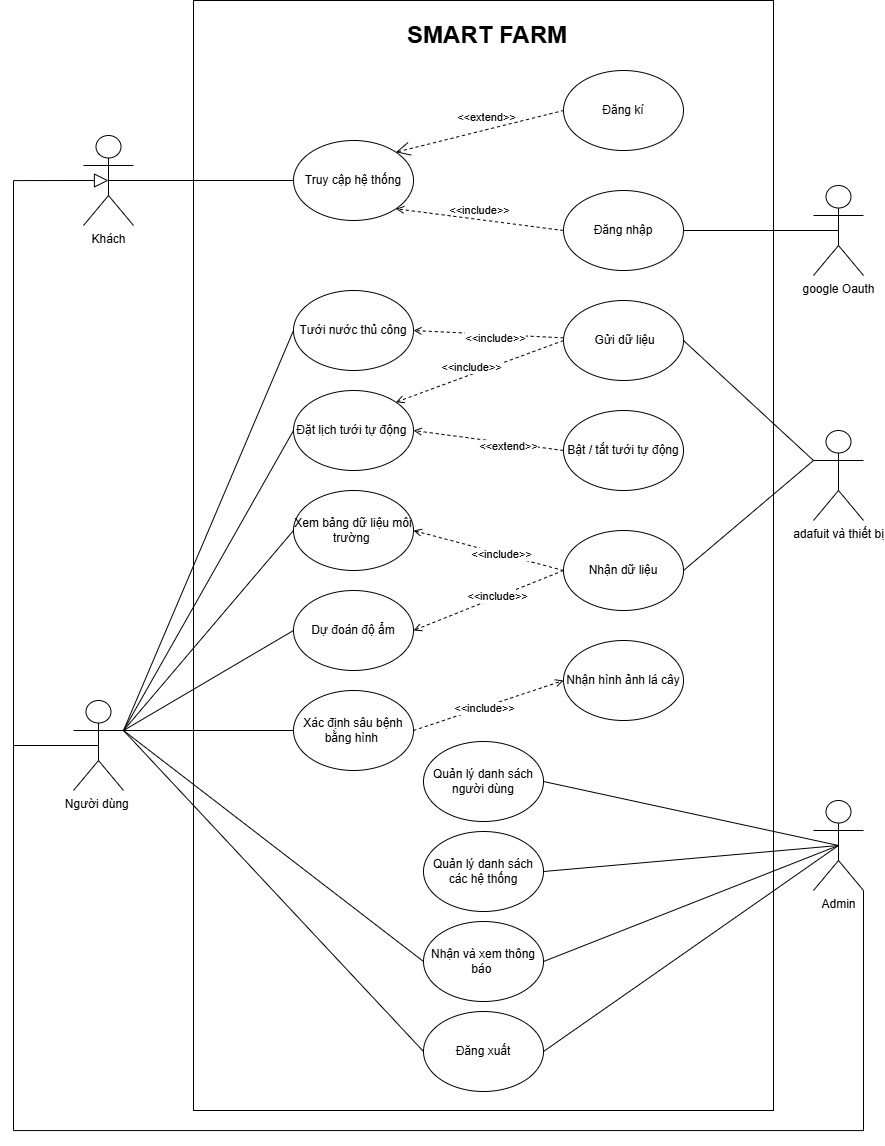
\includegraphics[width=0.8\linewidth]{./Pictures/Task_3/usecase.png}
	\caption{Use-case diagram -- Toàn bộ hệ thống}
\end{figure}
\subsubsection{Details (Scenario)}
%TODO
bsubsub{Truy cập hệ thống}
\setlist[enumerate]{leftmargin=*,topsep=0pt,itemsep=2pt,parsep=0pt}
\setlist[itemize]{leftmargin=*,topsep=0pt,itemsep=2pt,parsep=0pt}
\begin{longtable}{|P{4.8cm}|m{10cm}|}\hline 		
	\texttt{Use-case ID} & UC--01\\
	\hline
	%%%%%%%%%%%%%%%
	\texttt{Use-case Name} & Truy cập hệ thống\\
	\hline
	%%%%%%%%%%%%%%%
	\texttt{Use-case Overview} & Xác thực khách truy cập hệ thống và phân quyền người dùng.
	\\
	\hline
	\texttt{Actors} & Guest (Khách)
	\\
	\hline
	\texttt{Preconditions} & Khách truy cập hệ thống thành công và hệ thống hoạt động bình thường.
	\\
	\hline
	\texttt{Trigger} & Khách chọn nút đăng nhập hoặc đăng kí tài khoản.\\
	\hline
	\texttt{Basic flow} &
	\begin{enumerate}
		\item Khách truy cập hệ thống.
		\item Khách chọn hình thức đăng nhập (trực tiếp hoặc Google account)
		\item Nếu chọn đăng nhập trực tiếp, chọn mục ``Đăng nhập''.
		\item Khách nhập thông tin đăng nhập vào ô tương ứng (tên đăng nhập/ mật khẩu).
		\item Hệ thống đối chiếu thông tin đăng nhập của khách với dữ liệu được lưu ở database.
		\item Nếu khớp thông tin, hệ thống sẽ phân quyền cho khách là người dùng hoặc là admin.
		\item Chuyển người đó tới giao diện tương ứng với vai trò đã phân (user/ admin).
	\end{enumerate}
	\\
	\hline
	\texttt{Post conditions} & 
	Người dùng/ admin truy cập được hệ thống với giao diện tương ứng.
	\\
	\hline
	\texttt{Alterative flow} & 
	\begin{enumerate}[label = A\arabic*.]
		\item Ở bước 3, nếu chọn đăng nhập theo Google account thì hệ thống chuyển hướng người dùng đến trang xác thực của google và Google Oauth sẽ xác thực tài khoản.
		\item Ở bước 3, nếu chọn đăng nhập trực tiếp mà chưa có tài khoản thì khách chọn mục ``đăng kí'' để điền thông tin người dùng, tên đăng nhập và mật khẩu.
	\end{enumerate}
	\\
	\hline
	\texttt{Exception flow} & 
	\begin{enumerate}[label = E\arabic*:]
		\item Ở bước 6, nếu thông tin không khớp thì hệ thống báo lỗi ``tài khoản không đúng tên đăng nhập hoặc mật khẩu'' và khách phải nhập lại thông tin đăng nhập.
		\item Ở bước 7, nếu thông tin đăng nhập không khớp thì vẫn giữ nguyên màn hình đăng nhập.
	\end{enumerate}
	\\
	\hline
	\texttt{Special requirements} & Không có.\\
	\hline
	\texttt{Extension points} & Không có.\\
	\hline
	
	\caption{\label{table2}Đặc tả cho Use-case dự đoán độ ẩm}
\end{longtable}
\subsubsubsection{Dự đoán độ ẩm}
\setlist[enumerate]{leftmargin=*,topsep=0pt,itemsep=2pt,parsep=0pt}
\setlist[itemize]{leftmargin=*,topsep=0pt,itemsep=2pt,parsep=0pt}
\begin{longtable}{|P{4.8cm}|m{10cm}|}\hline 		
	\texttt{Use-case ID} & UC--02\\
	\hline
	%%%%%%%%%%%%%%%
	\texttt{Use-case Name} & Dự đoán độ ẩm\\
	\hline
	%%%%%%%%%%%%%%%
	\texttt{Use-case Overview} & Hệ thống dự đoán độ ẩm đất dựa trên dữ liệu từ cảm biến độ ẩm đất và cảm biến nhiệt độ -- độ ẩm DHT20
	\\
	\hline
	\texttt{Actors} & User
	\\
	\hline
	\texttt{Preconditions} & Hệ thống đã kết nối Internet và cảm biến hoạt động bình thường.
	\\
	\hline
	\texttt{Trigger} & Người dùng chọn chức năng dự đoán độ ẩm trên dashboard\\
	\hline
	\texttt{Basic flow} &
	\begin{enumerate}
		\item Người dùng truy cập dashboard.
		\item Người dùng chọn chức năng ``Dự đoán độ ẩm''.
		\item Hệ thống thu thập dữ liệu từ cảm biến độ ẩm đất.
		\item Hệ thống thu thập dữ liệu nhiệt độ và độ ẩm không khí từ cảm biến DHT20.
		\item Hệ thống gửi dữ liệu đến server xử lý.
		\item Server phân tích dữ liệu và thực hiện dự đoán độ ẩm đất.
		\item Server gửi kết quả dự đoán về hệ thống.
		\item Hệ thống hiển thị kết quả dự đoán trên dashboard.
	\end{enumerate}
	\\
	\hline
	\texttt{Post conditions} & 
	Hệ thống hiển thị kết quả dự đoán độ ẩm
	\\
	\hline
	\texttt{Alterative flow} & Tại bước 1 nếu hệ thống được cấu hình dự đoán tự động theo chu kỳ thì hệ thống tự động thu thập dữ liệu và thực hiện các bước 3 → 8 mà không cần người dùng kích hoạt.\\
	\hline
	\texttt{Exception flow} & 
	\begin{enumerate}[label = E\arabic*:]
		\item Tại bước 3 nếu cảm biến độ ẩm đất không gửi dữ liệu thì hệ thống hiển thị thông báo lỗi và dừng quá trình dự đoán.
		\item Tại bước 5 nếu hệ thống không kết nối được với server thì quá trình xử lý dữ liệu bị hủy và hệ thống hiển thị thông báo lỗi.
	\end{enumerate}
	\\
	\hline
	\texttt{Special requirements} & Không có.\\
	\hline
	\texttt{Extension points} & Không có.\\
	\hline
	
	\caption{\label{table3}Đặc tả cho Use-case dự đoán độ ẩm}
\end{longtable}
\subsubsubsection{Xác định sâu bệnh dựa trên hình ảnh}
%TODO
\setlist[enumerate]{leftmargin=*,topsep=0pt,itemsep=2pt,parsep=0pt}
\setlist[itemize]{leftmargin=*,topsep=0pt,itemsep=2pt,parsep=0pt}
\begin{longtable}{|P{4.8cm}|m{10cm}|}\hline 		
	\texttt{Use-case ID} & UC--03\\
	\hline
	%%%%%%%%%%%%%%%
	\texttt{Use-case Name} & Use-case Xác định sâu bệnh dựa trên hình ảnh\\
	\hline
	%%%%%%%%%%%%%%%
	\texttt{Use-case Overview} & Hệ thống nhận hình ảnh cây trồng từ người dùng hoặc camera và sử dụng mô hình AI để phân tích, xác định loại sâu bệnh có thể xuất hiện trên cây.
	\\
	\hline
	\texttt{Actors} & User
	\\
	\hline
	\texttt{Preconditions} & 
	\begin{enumerate}[label = \arabic*.]
		\item Hệ thống đã kết nối Internet.
		\item Camera hoặc chức năng tải ảnh hoạt động bình thường.
		\item Server AI sẵn sàng xử lý dữ liệu.
	\end{enumerate}
	\\
	\hline
	\texttt{Trigger} & Người dùng chọn chức năng ``Xác định sâu bệnh'' trên dashboard.\\
	\hline
	\texttt{Basic flow} &
	\begin{enumerate}
		\item Người dùng truy cập dashboard.
		\item Người dùng chọn chức năng ``Xác định sâu bệnh''.
		\item Người dùng chụp ảnh cây trồng hoặc tải ảnh từ thiết bị lên hệ thống.
		\item Hệ thống gửi hình ảnh đến server xử lý.
		\item Server phân tích hình ảnh bằng mô hình AI.
		\item Server xác định loại sâu bệnh (nếu có).
		\item Server gửi kết quả dự đoán về hệ thống.
		\item Hệ thống hiển thị kết quả nhận diện sâu bệnh trên dashboard.
	\end{enumerate}
	\\
	\hline
	\texttt{Post conditions} & 
	Hệ thống hiển thị kết quả nhận diện sâu bệnh và thông tin liên quan cho người dùng.
	\\
	\hline
	\texttt{Alterative flow} & Tại bước 3 nếu hệ thống được cấu hình sử dụng camera tự động thì camera sẽ định kỳ chụp ảnh và gửi lên server để phân tích mà không cần người dùng thực hiện.\\
	\hline
	\texttt{Exception flow} & 
	\begin{enumerate}[label = E\arabic*:]
		\item Tại bước 3 nếu người dùng không tải ảnh hoặc camera không hoạt động thì hệ thống hiển thị thông báo lỗi và yêu cầu thử lại.
		\item Tại bước 4 nếu hệ thống không gửi được dữ liệu đến server thì quá trình phân tích bị hủy và hệ thống hiển thị thông báo lỗi.
	\end{enumerate}
	\\
	\hline
	\texttt{Special requirements} & Không có.\\
	\hline
	\texttt{Extension points} & Không có.\\
	\hline
	
	\caption{\label{table4}Đặc tả cho Use-case Xác định sâu bệnh dựa trên hình ảnh}
\end{longtable}
\subsubsubsection{Xem bảng dữ liệu môi trường}
%TODO
\setlist[enumerate]{leftmargin=*,topsep=0pt,itemsep=2pt,parsep=0pt}
\setlist[itemize]{leftmargin=*,topsep=0pt,itemsep=2pt,parsep=0pt}
\begin{longtable}{|P{4.8cm}|m{10cm}|}\hline 		
	\texttt{Use-case ID} & UC--04\\
	\hline
	%%%%%%%%%%%%%%%
	\texttt{Use-case Name} & Xem bảng dữ liệu môi trường\\
	\hline
	%%%%%%%%%%%%%%%
	\texttt{Use-case Overview} & Người dùng xem các thông số môi trường được thu thập từ hệ thống cảm biến như nhiệt độ không khí, độ ẩm không khí và độ ẩm đất.
	\\
	\hline
	\texttt{Actors} & User
	\\
	\hline
	\texttt{Preconditions} & Hệ thống đang thu thập dữ liệu từ cảm biến
	\\
	\hline
	\texttt{Trigger} & Người dùng truy cập dashboard\\
	\hline
	\texttt{Basic flow} &
	\begin{enumerate}
		\item Người dùng truy cập dashboard.
		\item Hệ thống yêu cầu dữ liệu từ các cảm biến.
		\item Hệ thống nhận dữ liệu nhiệt độ và độ ẩm không khí từ cảm biến.
		\item Hệ thống nhận dữ liệu từ cảm biến độ ẩm đất.
		\item Hệ thống xử lý dữ liệu.
		\item Hệ thống hiển thị dữ liệu trên dashboard dưới dạng bảng hoặc biểu đồ.
	\end{enumerate}
	\\
	\hline
	\texttt{Post conditions} & 
	Dữ liệu môi trường được hiển thị cho người dùng
	\\
	\hline
	\texttt{Alterative flow} & Tại bước 6 nếu người dùng chọn xem dữ liệu lịch sử thì hệ thống hiển thị biểu đồ dữ liệu môi trường theo thời gian.\\
	\hline
	\texttt{Exception flow} & 
	\begin{enumerate}[label = E\arabic*:]
		\item Tại bước 3 hoặc bước 4 nếu hệ thống không nhận được dữ liệu từ cảm biến thì dashboard hiển thị trạng thái ``No Data''.
		\item Tại bước 2 nếu dashboard không kết nối được server thì dữ liệu không thể hiển thị và hệ thống thông báo lỗi.
	\end{enumerate}
	\\
	\hline
	\texttt{Special requirements} & Không có.\\
	\hline
	\texttt{Extension points} & Không có.\\
	\hline
	
	\caption{\label{table5}Đặc tả cho Use-case Xem bảng dữ liệu môi trường}
\end{longtable}
\subsubsubsection{Tưới nước thủ công}
%TODO
\setlist[enumerate]{leftmargin=*,topsep=0pt,itemsep=2pt,parsep=0pt}
\setlist[itemize]{leftmargin=*,topsep=0pt,itemsep=2pt,parsep=0pt}
\begin{longtable}{|P{4.8cm}|m{10cm}|}\hline 		
	\texttt{Use-case ID} & UC--05\\
	\hline
	%%%%%%%%%%%%%%%
	\texttt{Use-case Name} & Use-case Tưới nước thủ công\\
	\hline
	%%%%%%%%%%%%%%%
	\texttt{Use-case Overview} & Người dùng có thể chủ động bật hoặc tắt hệ thống tưới nước thông qua dashboard để tưới cây ngay lập tức.
	\\
	\hline
	\texttt{Actors} & User
	\\
	\hline
	\texttt{Preconditions} & 
	\begin{enumerate}[label = \arabic*.]
		\item Hệ thống đang hoạt động bình thường.
		\item Người dùng đã truy cập dashboard.
		\item Máy bơm nước được kết nối với hệ thống.
	\end{enumerate}
	\\
	\hline
	\texttt{Trigger} & Người dùng chọn chức năng ``Tưới nước thủ công'' trên dashboard.\\
	\hline
	\texttt{Basic flow} &
	\begin{enumerate}
		\item Người dùng truy cập dashboard.
		\item Người dùng chọn chức năng ``Tưới nước thủ công''.
		\item Hệ thống hiển thị nút điều khiển bật/tắt máy bơm.
		\item Người dùng chọn bật máy bơm.
		\item Hệ thống gửi tín hiệu điều khiển đến bộ điều khiển máy bơm.
		\item Máy bơm bắt đầu hoạt động và tưới cây.
		\item Khi người dùng chọn tắt máy bơm, hệ thống gửi tín hiệu dừng.
		\item Máy bơm ngừng hoạt động.
	\end{enumerate}
	\\
	\hline
	\texttt{Post conditions} & 
	Máy bơm nước được kích hoạt hoặc tắt theo thao tác của người dùng.
	\\
	\hline
	\texttt{Alterative flow} & Tại bước 4 nếu người dùng đặt thời gian tưới cụ thể thì hệ thống tự động tắt máy bơm sau khi hết thời gian đã chọn.\\
	\hline
	\texttt{Exception flow} & 
	\begin{enumerate}[label = E\arabic*:]
		\item Tại bước 5 nếu hệ thống không gửi được tín hiệu điều khiển đến máy bơm thì hệ thống hiển thị thông báo lỗi.
		\item Tại bước 6 nếu máy bơm không phản hồi thì hệ thống hiển thị trạng thái lỗi và yêu cầu người dùng kiểm tra thiết bị.
	\end{enumerate}
	\\
	\hline
	\texttt{Special requirements} & Không có.\\
	\hline
	\texttt{Extension points} & Không có.\\
	\hline
	
	\caption{\label{table6}Đặc tả cho Use-case Tưới nước thủ công}
\end{longtable}

\subsubsubsection{Đặt lịch tưới nước tự động}
%TODO
\setlist[enumerate]{leftmargin=*,topsep=0pt,itemsep=2pt,parsep=0pt}
\setlist[itemize]{leftmargin=*,topsep=0pt,itemsep=2pt,parsep=0pt}
\begin{longtable}{|P{4.8cm}|m{10cm}|}\hline 		
	\texttt{Use-case ID} & UC--06\\
	\hline
	%%%%%%%%%%%%%%%
	\texttt{Use-case Name} & Đặt lịch tưới nước tự động\\
	\hline
	%%%%%%%%%%%%%%%
	\texttt{Use-case Overview} & Người dùng thiết lập lịch tưới nước tự động cho hệ thống. Khi đến thời gian đã đặt, hệ thống sẽ kích hoạt máy bơm để tưới cây.
	\\
	\hline
	\texttt{Actors} & User
	\\
	\hline
	\texttt{Preconditions} & Hệ thống đã kết nối Internet và máy bơm nước hoạt động bình thường.
	\\
	\hline
	\texttt{Trigger} & Người dùng chọn chức năng đặt lịch tưới nước\\
	\hline
	\texttt{Basic flow} &
	\begin{enumerate}
		\item Người dùng truy cập dashboard.
		\item Người dùng chọn chức năng ``Đặt lịch tưới nước''.
		\item Người dùng nhập thời gian bắt đầu và thời gian tưới.
		\item Hệ thống lưu lịch tưới.
		\item Khi đến thời gian đã đặt, hệ thống kích hoạt máy bơm nước.
		\item Sau khi hết thời gian tưới, hệ thống tắt máy bơm.
	\end{enumerate}
	\\
	\hline
	\texttt{Post conditions} & 
	Lịch tưới được lưu và hệ thống thực hiện tưới tự động
	\\
	\hline
	\texttt{Alterative flow} & 
	\begin{enumerate}[label = A\arabic*:]
		\item Tại bước 4 nếu người dùng muốn thay đổi lịch tưới thì hệ thống cho phép chỉnh sửa và lưu lại lịch mới.
		\item Tại bước 2 nếu người dùng tắt chế độ tưới tự động thì hệ thống không thực hiện lịch tưới đã đặt.
	\end{enumerate}
	\\
	\hline
	\texttt{Exception flow} & 
	\begin{enumerate}[label = E\arabic*:]
		\item Tại bước 3 nếu thời gian người dùng nhập không hợp lệ thì hệ thống yêu cầu người dùng nhập lại.
		\item Tại bước 5 nếu máy bơm không phản hồi thì hệ thống hiển thị thông báo lỗi và không thực hiện tưới nước.
	\end{enumerate}
	\\
	\hline
	\texttt{Special requirements} & Không có.\\
	\hline
	\texttt{Extension points} & Không có.\\
	\hline
	
	\caption{\label{table7}Đặc tả cho Use-case Đặt lịch tưới nước tự động}
\end{longtable}
\subsubsubsection{Nhận và xem thông báo}
%TODO
\setlist[enumerate]{leftmargin=*,topsep=0pt,itemsep=2pt,parsep=0pt}
\setlist[itemize]{leftmargin=*,topsep=0pt,itemsep=2pt,parsep=0pt}
\begin{longtable}{|P{4.8cm}|m{10cm}|}\hline 		
	\texttt{Use-case ID} & UC--07\\
	\hline
	%%%%%%%%%%%%%%%
	\texttt{Use-case Name} & Use-case Nhận và xem thông báo\\
	\hline
	%%%%%%%%%%%%%%%
	\texttt{Use-case Overview} & Hệ thống gửi thông báo đến người dùng khi xảy ra các sự kiện quan trọng như độ ẩm đất thấp, phát hiện sâu bệnh, lỗi cảm biến hoặc hệ thống tưới nước. Hoặc gửi thông báo đến admin về những thay đổi mà admin đã thực hiện.
	\\
	\hline
	\texttt{Actors} & User, Admin
	\\
	\hline
	\texttt{Preconditions} & 
	\begin{enumerate}[label = \arabic*.]
		\item Hệ thống đã kết nối Internet.
		\item Người dùng/ admin đã đăng nhập vào hệ thống.
	\end{enumerate}
	\\
	\hline
	\texttt{Trigger} & Hệ thống phát hiện một sự kiện cần thông báo.\\
	\hline
	\texttt{Basic flow} &
	\begin{enumerate}
		\item Hệ thống phát hiện sự kiện cần thông báo.
		\item Hệ thống tạo thông báo với nội dung tương ứng.
		\item Hệ thống gửi thông báo đến dashboard hoặc ứng dụng của người dùng hoặc admin.
		\item Người dùng hoặc admin mở mục thông báo trên dashboard.
		\item Hệ thống hiển thị danh sách các thông báo.
		\item Người dùng hoặc admin chọn một thông báo để xem chi tiết.
	\end{enumerate}
	\\
	\hline
	\texttt{Post conditions} & 
	Người dùng hoặc admin nhận được và xem nội dung thông báo.
	\\
	\hline
	\texttt{Alterative flow} & Tại bước 3 nếu người dùng bật thông báo qua email hoặc ứng dụng di động thì hệ thống gửi thông báo qua các kênh này.\\
	\hline
	\texttt{Exception flow} & 
	\begin{enumerate}[label = E\arabic*:]
		\item Tại bước 3 nếu hệ thống không kết nối được Internet thì thông báo sẽ được lưu lại và gửi khi kết nối được khôi phục.
		\item Tại bước 4 nếu người dùng chưa đăng nhập thì hệ thống yêu cầu đăng nhập trước khi xem thông báo.
	\end{enumerate}
	\\
	\hline
	\texttt{Special requirements} & Không có.\\
	\hline
	\texttt{Extension points} & Không có.\\
	\hline
	
	\caption{\label{table8}Đặc tả cho Use-case Nhận và xem thông báo}
\end{longtable}

\subsubsubsection{Đăng xuất}
%TODO
\setlist[enumerate]{leftmargin=*,topsep=0pt,itemsep=2pt,parsep=0pt}
\setlist[itemize]{leftmargin=*,topsep=0pt,itemsep=2pt,parsep=0pt}
\begin{longtable}{|P{4.8cm}|m{10cm}|}\hline 		
	\texttt{Use-case ID} & UC--08\\
	\hline
	%%%%%%%%%%%%%%%
	\texttt{Use-case Name} & Use-case Đăng xuất\\
	\hline
	%%%%%%%%%%%%%%%
	\texttt{Use-case Overview} & Người dùng/ admin chọn đăng xuất, hệ thống hiển thị lại màn hình đăng nhập và xóa bỏ phân quyền người dùng hiện tại.
	\\
	\hline
	\texttt{Actors} & User, admin
	\\
	\hline
	\texttt{Preconditions} & 
	\begin{enumerate}[label = \arabic*.]
		\item Người dùng đã đăng nhập vào hệ thống.
		\item Người dùng, admin đang ở trong hệ thống.
	\end{enumerate}
	\\
	\hline
	\texttt{Trigger} & Người dùng/ admin nhấn vào nút ``đăng xuất''.\\
	\hline
	\texttt{Basic flow} &
	\begin{enumerate}
		\item Người dùng/ admin nhấn vào nút đăng xuất.
		\item Hệ thống hiển thị thông báo yêu cầu xác nhận việc đăng xuất.
		\item Nếu chấp nhận, hệ thống xóa bỏ phân quyền hiện tại và chuyển hướng về giao diện đăng nhập.
	\end{enumerate}
	\\
	\hline
	\texttt{Post conditions} & 
	Người dùng/ admin bị xóa bỏ phân quyền và trở lại là khách; hệ thống chuyển hướng về màn hình đăng nhập.
	\\
	\hline
	\texttt{Alterative flow} & Tại bước 3, nếu không chấp nhận thì hệ thống hủy bỏ việc đăng xuất và vẫn giữ nguyên quyền của người dùng này.\\
	\hline
	\texttt{Exception flow} & 
	Không có
	\\
	\hline
	\texttt{Special requirements} & Không có.\\
	\hline
	\texttt{Extension points} & Không có.\\
	\hline
	
	\caption{\label{table9}Đặc tả cho Use-case Đăng xuất}
\end{longtable}
\subsection{Use-case chi tiết cho role Admin}
\subsubsection{Diagram}
%TODO
\begin{figure}[H]
	\centering
	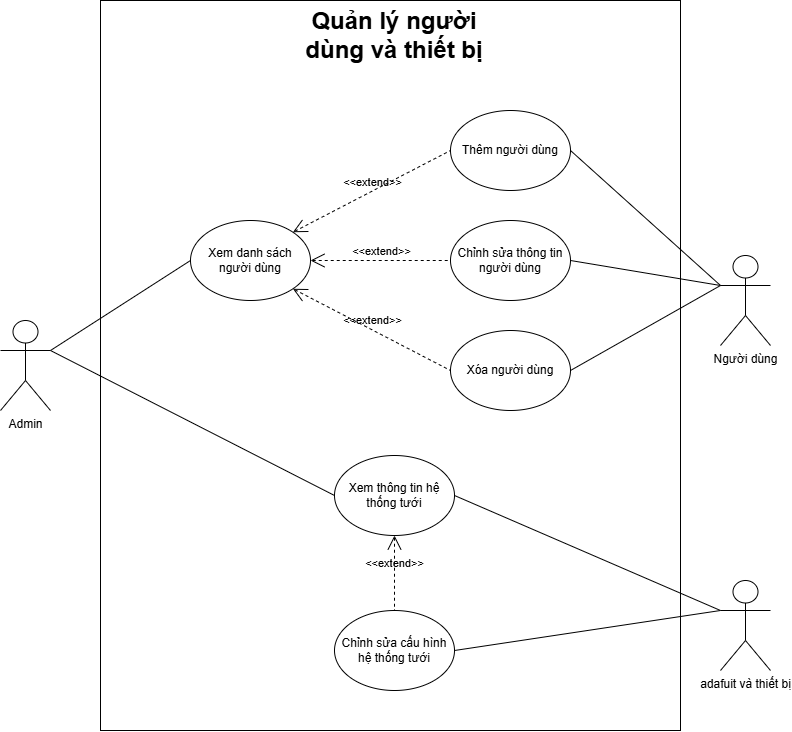
\includegraphics[width=0.8\linewidth]{./Pictures/Task_3/usecase_admin.png}
	\caption{Use-case diagram -- chi tiết cho role Admin}
\end{figure}

\subsubsection{Details (Scenario)}
%TODO
\subsubsubsection{Xem danh sách người dùng}
\setlist[enumerate]{leftmargin=*,topsep=0pt,itemsep=2pt,parsep=0pt}
\setlist[itemize]{leftmargin=*,topsep=0pt,itemsep=2pt,parsep=0pt}
\begin{longtable}{|P{4.8cm}|m{10cm}|}\hline 		
	\texttt{Use-case ID} & UC--B01\\
	\hline
	%%%%%%%%%%%%%%%
	\texttt{Use-case Name} & Xem danh sách người dùng\\
	\hline
	%%%%%%%%%%%%%%%
	\texttt{Use-case Overview} & Admin có thể xem danh sách các người dùng đã đăng kí tài khoản vào hệ thống, ngoài ra còn có thể thêm người dùng, chỉnh sửa thông tin hoặc xóa tài khoản người dùng đã đăng kí trước đó.
	\\
	\hline
	\texttt{Actors} & Admin, users
	\\
	\hline
	\texttt{Preconditions} & Admin đăng nhập thành công vào hệ thống.
	\\
	\hline
	\texttt{Trigger} & Admin truy cập vào mục quản lý người dùng.\\
	\hline
	\texttt{Basic flow} &
	\begin{enumerate}
		\item Admin truy cập vào mục quản lý người dùng.
		\item Admin chọn các chức năng đặc quyền: thêm, chỉnh sửa thông tin, xóa người dùng.
		\item Nếu chọn thêm người dùng, admin có thể tạo một tài khoản người dùng mới bằng việc thêm tên đăng nhập, mật khẩu tương ứng. Hệ thống ghi nhận và thêm vào cơ sở dữ liệu.
	\end{enumerate}
	\\
	\hline
	\texttt{Post conditions} & 
	Hệ thống cập nhật lại thông tin tương ứng mà admin đã thao tác.
	\\
	\hline
	\texttt{Alterative flow} & 
	\begin{enumerate}[label = A\arabic*.]
		\item Ở bước 3, nếu admin chọn chỉnh sửa thông tin người dùng thì admin có thể chỉnh sửa thông tin cá nhân, tên đăng nhập và mật khẩu người dùng.
		\item Ở bước 3, nếu admin chọn xoá người dùng thì hệ thống sẽ xóa toàn bộ thông tin của người dùng trong cơ sở dữ liệu.
	\end{enumerate}
	\\
	\hline
	\texttt{Exception flow} & 
	\begin{enumerate}[label = E\arabic*:]
		\item Ở bước 2, nếu admin tìm thông tin của người dùng không tồn tại trong cơ sở dữ liệu hiện tại thì hệ thống báo lỗi.
	\end{enumerate}
	\\
	\hline
	\texttt{Special requirements} & Không có.\\
	\hline
	\texttt{Extension points} & Không có.\\
	\hline
	
	\caption{\label{table10}Đặc tả cho Use-case Xem danh sách người dùng}
\end{longtable}

\subsubsubsection{Xem danh sách người dùng}
\setlist[enumerate]{leftmargin=*,topsep=0pt,itemsep=2pt,parsep=0pt}
\setlist[itemize]{leftmargin=*,topsep=0pt,itemsep=2pt,parsep=0pt}
\begin{longtable}{|P{4.8cm}|m{10cm}|}\hline 		
	\texttt{Use-case ID} & UC--B02\\
	\hline
	%%%%%%%%%%%%%%%
	\texttt{Use-case Name} & Xem thông tin hệ thống tưới\\
	\hline
	%%%%%%%%%%%%%%%
	\texttt{Use-case Overview} & Admin có thể xem và chỉnh sửa các thông số của các thiết bị cũng như cách bố trí các thành phần trong hệ thống.
	\\
	\hline
	\texttt{Actors} & Admin, adafruit và thiết bị
	\\
	\hline
	\texttt{Preconditions} & Admin đăng nhập thành công vào hệ thống.
	\\
	\hline
	\texttt{Trigger} & Admin truy cập vào mục ``quản lý thiết bị và hệ thống''.\\
	\hline
	\texttt{Basic flow} &
	\begin{enumerate}
		\item Admin truy cập vào mục ``quản lý thiết bị và hệ thống''.
		\item Admin chọn mục xem thông tin hệ thống tưới.
		\item Hệ thống truy xuất dữ liệu cấu hình thiết bị từ Adafruit và cơ sở dữ liệu.
		\item Hệ thống hiển thị danh sách các thiết bị trong hệ thống tưới (cảm biến độ ẩm đất, cảm biến DHT20, máy bơm nước) cùng với trạng thái hoạt động và các thông số cấu hình hiện tại.
		\item Admin xem chi tiết thông tin của từng thiết bị bao gồm: tên thiết bị, trạng thái kết nối, giá trị đọc được, ngưỡng hoạt động và lịch sử hoạt động.
	\end{enumerate}
	\\
	\hline
	\texttt{Post conditions} & 
	Hệ thống cập nhật lại thông tin tương ứng mà admin đã thao tác.
	\\
	\hline
	\texttt{Alterative flow} & 
	\begin{enumerate}[label = A\arabic*.]
		\item Ở bước 5, nếu admin chọn chỉnh sửa cấu hình hệ thống tưới thì hệ thống cho phép admin thay đổi các thông số như: ngưỡng độ ẩm kích hoạt tưới, thời gian tưới, tần suất đọc cảm biến. Sau khi chỉnh sửa, hệ thống gửi cấu hình mới đến Adafruit để cập nhật cho thiết bị.
	\end{enumerate}
	\\
	\hline
	\texttt{Exception flow} & 
	\begin{enumerate}[label = E\arabic*:]
		\item Ở bước 3, nếu hệ thống không kết nối được tới Adafruit thì báo lỗi.
	\end{enumerate}
	\\
	\hline
	\texttt{Special requirements} & Không có.\\
	\hline
	\texttt{Extension points} & Không có.\\
	\hline
	
	\caption{\label{table11}Đặc tả cho Use-case Xem thông tin hệ thống tưới}
\end{longtable}
	\section{Adafruit và thiết bị}
\subsection{Adafruit}
\subsubsection{Adafruit IO}
\indent Adafruit IO là một nền tảng IoTs (Internet of Things) dựa trên đám mây, giúp bạn thu thập, hiển thị và điều khiển dữ liệu từ các thiết bị kết nối internet. Đây là một dịch vụ miễn phí của Adafruit, hỗ trợ các giao thức REST API và MQTT, giúp dễ dàng kết nối các vi điều khiển như ESP8266, ESP32, Raspberry Pi, Arduino, STM32,...
\subsubsection{Các chức năng chính của Adafruit IO}
\begin{itemize}[leftmargin = 1cm]
	\item \textit{Feeds (Luồng dữ liệu):} Lưu trữ và quản lý dữ liệu từ cảm biến hoặc thiết bị.
	\item \textit{Dashboards (Bảng điều khiển):} Cung cấp giao diện đồ họa trực quan (biểu đồ, công tắc, nút bấm,...) để giám sát dữ liệu. Có thể tạo dashboard để điều khiển thiết bị từ xa.
	\item \textit{Giao thức MQTT:} Gửi dữ liệu theo thời gian thực, phù hợp với thiết bị IoT.
	\item \textit{Hỗ trợ nhiều nền tảng:} Có thư viện Adafruit IO Arduino và Adafruit MQTT giúp lập trình dễ dàng. Tích hợp với ESP8266, ESP32, Arduino, Raspberry Pi, STM32, Python,...
\end{itemize}
\subsubsection{Cách hoạt động của Adafruit IO}
\begin{itemize}[leftmargin = 1cm]
	\item Thiết bị IoT (ESP8266, ESP32,...) gửi dữ liệu lên Adafruit IO qua MQTT hoặc REST API.
	\item Adafruit IO lưu trữ và hiển thị dữ liệu trên giao diện trên feed.
	\item Người dùng có thể điều khiển thiết bị từ xa qua dashboard hoặc API. Tức là điều khiển thiết bị IoT bằng cách ra lệnh cho Adafruit IO thông qua Adafruit dashboard.
\end{itemize}

\subsection{Thiết kế hệ thống và lựa chọn thiết bị}
\indent Ở giai đoạn đầu, nhóm tiến hành phân tích yêu cầu của hệ thống nông nghiệp thông minh và lựa chọn các thiết bị phù hợp. Hệ thống được thiết kế gồm các thành phần chính:
\begin{itemize}[leftmargin = 1cm]
	\item \textbf{Cảm biến DHT20:} dùng để đo nhiệt độ và độ ẩm không khí.
	Cảm biến này cung cấp dữ liệu môi trường nền để hệ thống đánh giá điều kiện phát triển của cây và cập nhật lên dashboard.
	\begin{figure}[H]
		\centering
		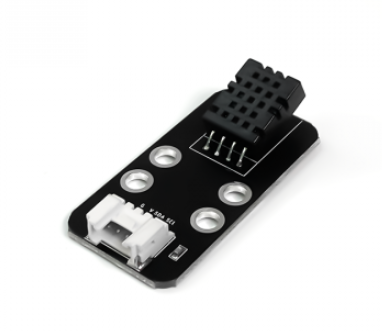
\includegraphics[width=0.45\linewidth]{./Pictures/Task_4/1_dht20.png}
		\caption{Cảm biến DHT20}
	\end{figure}
	\item \textbf{Cảm biến độ ẩm đất:} dùng để xác định tình trạng đất nhằm hỗ trợ hệ thống tưới tự động.
	Cảm biến giúp nhận biết đất đang khô hay đủ ẩm, từ đó làm căn cứ kích hoạt tưới nước hợp lý.
	\begin{figure}[H]
		\centering
		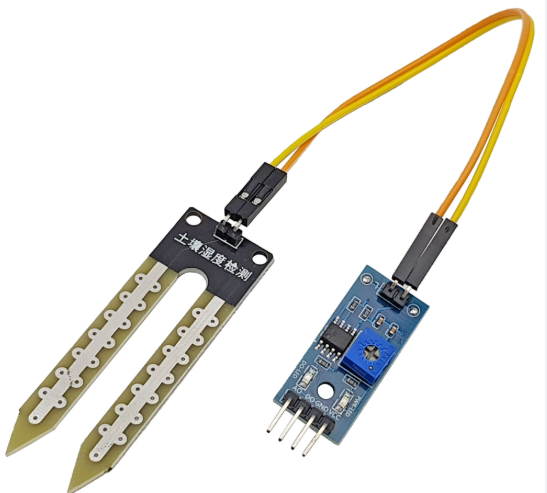
\includegraphics[width=0.45\linewidth]{./Pictures/Task_4/2_cb_doAmDat.png}
		\caption{Cảm biến độ ẩm đất}
	\end{figure}
	\item \textbf{Cảm biến ánh sáng:} để theo dõi cường độ ánh sáng trong môi trường.
	Dữ liệu từ cảm biến được dùng để kiểm tra mức chiếu sáng tại khu vực trồng và hỗ trợ đánh giá nhu cầu bổ sung ánh sáng.
	\begin{figure}[H]
		\centering
		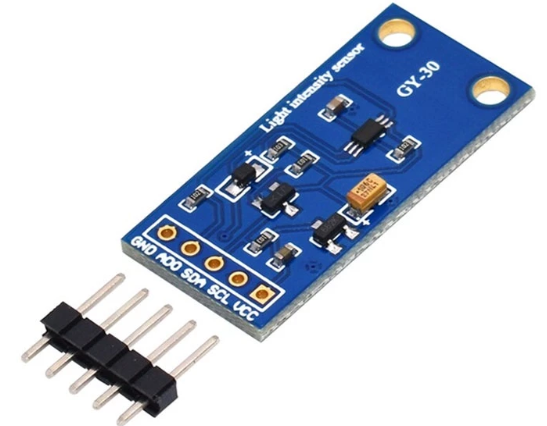
\includegraphics[width=0.45\linewidth]{./Pictures/Task_4/3_cb_anhSang.png}
		\caption{Cảm biến ánh sáng}
	\end{figure}
	\item \textbf{Đèn RGB:} dùng làm đèn báo trạng thái của hệ thống.
	Đèn RGB được dùng để hiển thị trạng thái hoạt động bằng màu sắc, giúp người dùng quan sát nhanh tình trạng hệ thống ngay tại thiết bị.
	\begin{figure}[H]
		\centering
		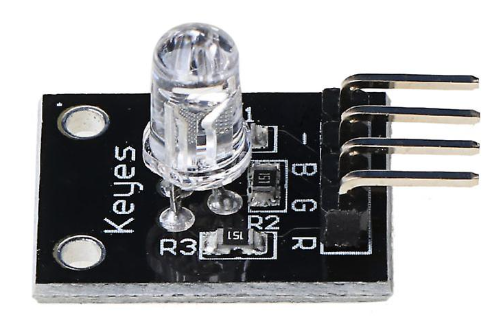
\includegraphics[width=0.45\linewidth]{./Pictures/Task_4/4_denRGB.png}
		\caption{Đèn RGB}
	\end{figure}
	\item \textbf{Màn hình LCD 16$\times$2:} để hiển thị các thông số môi trường trực tiếp tại thiết bị.
	Màn hình này cho phép quan sát trực tiếp các giá trị đo được mà không cần truy cập vào giao diện web.
	\begin{figure}[H]
		\centering
		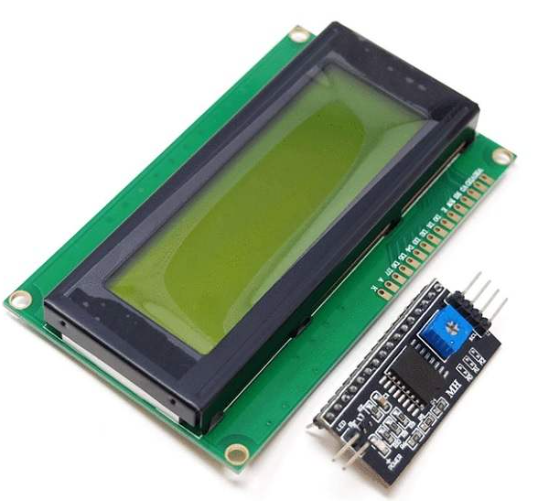
\includegraphics[width=0.45\linewidth]{./Pictures/Task_4/5_manHinhLCD.png}
		\caption{Màn hình LCD 16$\times$2}
	\end{figure}
	\item \textbf{Hai máy bơm nước:} phục vụ chức năng tưới tự động và tưới theo thời gian.
	Hai máy bơm đóng vai trò chấp hành, đưa nước đến cây trồng khi hệ thống cần tưới hoặc theo lịch đã thiết lập.
	\begin{figure}[H]
		\centering
		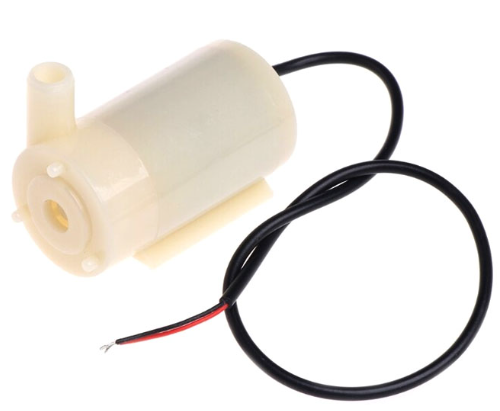
\includegraphics[width=0.45\linewidth]{./Pictures/Task_4/6_mayBom.png}
		\caption{Máy bơm mini}
	\end{figure}
\end{itemize}

\subsection{Kết nối phần cứng}
\indent Sau khi lựa chọn thiết bị, nhóm tiến hành thiết kế sơ đồ kết nối phần cứng. Trong hệ thống này, Yolo:Bit đóng vai trò là bộ điều khiển trung tâm, nhận dữ liệu từ các cảm biến, xử lý logic điều khiển và xuất tín hiệu đến các cơ cấu chấp hành, đồng thời là cầu nối giữa lớp phần cứng và lớp IoT.
\begin{figure}[H]
	\centering
	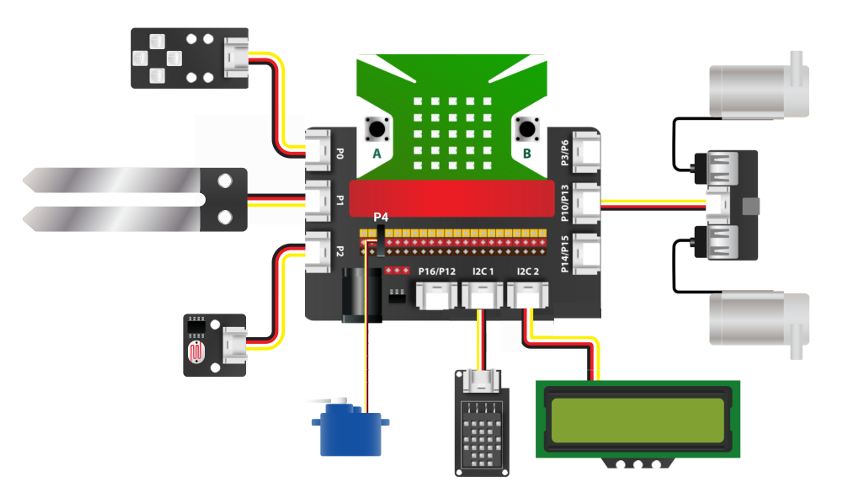
\includegraphics[width=1\linewidth]{./Pictures/Task_4/8_YoloBit_circuit.png}
	\caption{Kết nối thêm ngoại vi cho Yolo:Bit}
\end{figure}

\begin{itemize}[leftmargin = 1cm]
	\item \textbf{DHT20} được kết nối qua \textbf{I2C1} để đọc nhiệt độ và độ ẩm, là đầu vào chính cho việc giám sát môi trường.
	\item \textbf{LCD 16x2} sử dụng \textbf{I2C2} để hiển thị dữ liệu, giúp người dùng theo dõi thông số ngay tại thiết bị.
	\item \textbf{Cảm biến độ ẩm đất} được kết nối tại \textbf{P1} để đo tình trạng ẩm của đất phục vụ tưới tự động.
	\item \textbf{Cảm biến ánh sáng} được kết nối tại \textbf{P2} để ghi nhận cường độ chiếu sáng môi trường.
	\item \textbf{Đèn RGB} được kết nối tại \textbf{P0} để báo trạng thái hoạt động của hệ thống.
	\item \textbf{Động cơ RC} được điều khiển thông qua \textbf{P4} như một cơ cấu chấp hành trong quá trình vận hành.
	\item \textbf{Hai máy bơm} được điều khiển qua \textbf{P10} và \textbf{P13} để thực hiện chức năng tưới nước.
\end{itemize}
\indent Sau khi hoàn thành kết nối, hệ thống phần cứng đã hoạt động ổn định và có thể đọc dữ liệu từ các cảm biến.
\subsection{Thiết kế dashboard giám sát}
\begin{figure}[H]
	\centering
	
\includegraphics[width=1\linewidth]{./Pictures/Task_4/9_dashboard.png}
	\caption{Adafruit dashboard giám sát hệ thống}
\end{figure}
\indent Sau khi hoàn thành giao tiếp với server, nhóm tiến hành thiết kế Dashboard trên Adafruit IO để giám sát và điều khiển hệ thống từ xa.\\
\indent Dashboard bao gồm các \textit{gauges} để hiển thị giá trị tức thời, các \textit{cards} cho thông số quan trọng, các \textit{charts} để theo dõi lịch sử dữ liệu và các \textit{buttons} để điều khiển LED, máy bơm từ xa.
\begin{enumerate}[label = \arabic*., leftmargin = 1.7cm]
	\item Đồng hồ hiển thị nhiệt độ và độ ẩm.
	\item Đồng hồ hiển thị độ ẩm đất và cường độ ánh sáng.
	\item Các biểu đồ lịch sử dữ liệu cho nhiệt độ, độ ẩm và ánh sáng.
	\item Nút điều khiển LED và máy bơm từ xa.
\end{enumerate}
$\Longrightarrow$ Giao diện này cho phép người dùng theo dõi trạng thái môi trường và điều khiển thiết bị theo thời gian thực.
	\section{Hiện thực hệ thống}
\subsection{Triển khai phần mềm}
\subsubsection{Giới thiệu}
\indent Nhằm hiện thực một hệ thống có khả năng điều khiển các thiết bị phần cứng từ xa một cách thủ công hoặc tự động qua thiết lập lịch, đồng thời xem số liệu trực tiếp từ các cảm biến và hỗ trợ dự đoán loại bệnh của lá cây, nhóm đã xây dựng ứng dụng web SmartFarm. SmartFarm là hệ thống nông nghiệp thông minh kết hợp sức mạnh của \textbf{Trí tuệ nhân tạo (AI)} và \textbf{Internet vạn vật (IoT)}, cung cấp cho người dùng khả năng giám sát trạng thái môi trường và quản lý thiết bị trang trại từ mọi nơi thông qua một giao diện web trực quan, hiện đại. Hệ thống được triển khai theo mô hình client-server tiên tiến, đảm bảo đồng bộ hóa dữ liệu thời gian thực và tự động hóa các quy trình tưới tiêu, chiếu sáng, mang lại hiệu quả cao nhất cho sản xuất nông nghiệp.
\begin{figure}[H]
    \centering
    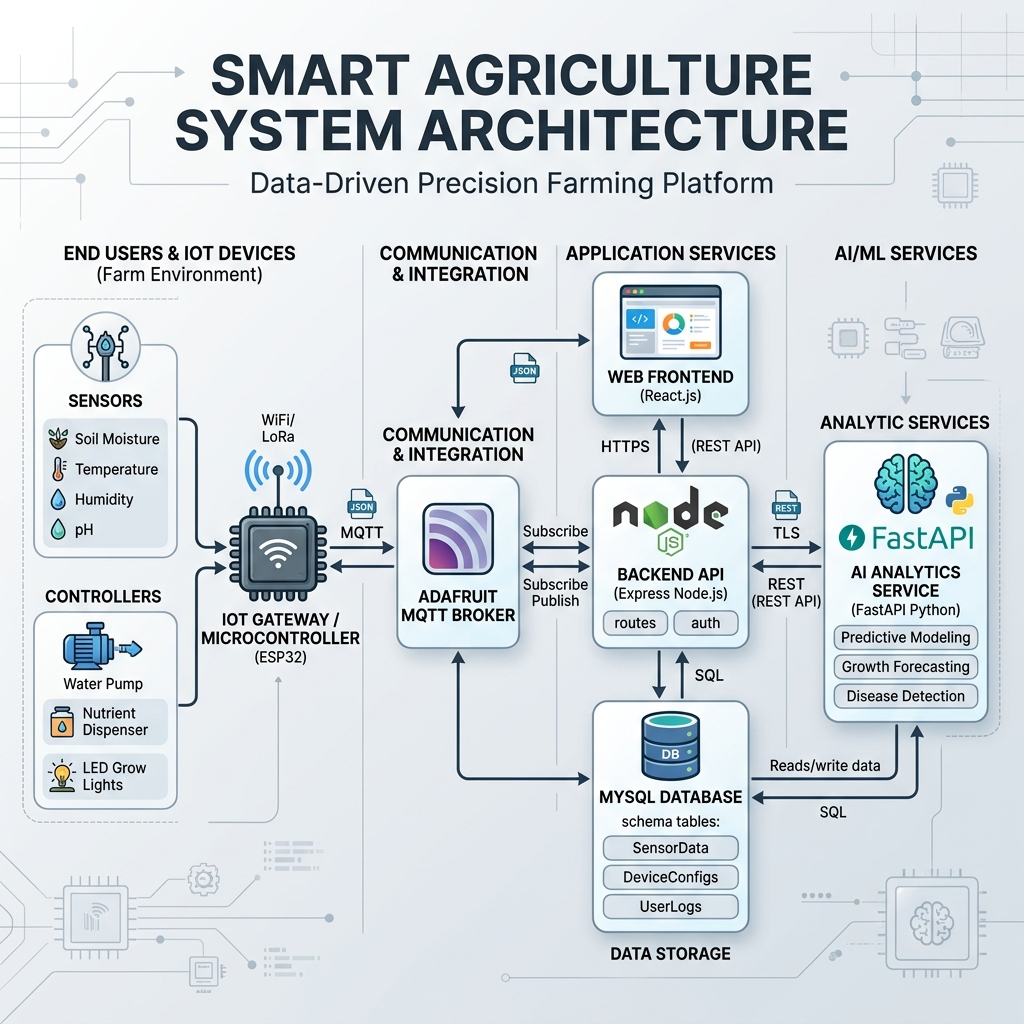
\includegraphics[width=0.75\linewidth]{./Pictures/Task_5/structure.png}
    \caption{Kiến trúc hệ thống SmartFarm}
\end{figure}

\begin{itemize}
    \item \textbf{Frontend}: React 19 + TypeScript + Vite
    \item \textbf{Backend}: Node.js + Express + Socket.IO
    \item \textbf{AI API}: FastAPI + TensorFlow/Keras (Python 3.10--3.12)
    \item \textbf{Database}: MySQL (mysql2)
    \item \textbf{IoT}: Adafruit IO (MQTT)
    \item \textbf{AI Model}: EfficientNet --- nhận diện 6 loại bệnh trên lá cà chua
\end{itemize}

\subsubsection{Tổng quan}
    \begin{longtable}{|P{0.35\linewidth}|m{0.58\linewidth}|}
        \hline
        \textbf{Tính năng} & \begin{center}\textbf{Mô tả}\end{center} \\
        \hline
        \textbf{Dashboard} & Giám sát cảm biến thời gian thực (nhiệt độ, độ ẩm, ánh sáng, độ ẩm đất) \\
        \hline
        \textbf{Điều khiển thiết bị} & Bật/tắt bơm nước, đèn LED, servo từ xa \\
        \hline
        \textbf{Lịch trình tưới tự động} & Lịch tưới theo ngày lặp lại, khoảng thời gian bắt đầu/kết thúc \\
        \hline
        \textbf{AI Phát hiện sâu bệnh} & Upload ảnh lá cây $\rightarrow$ mô hình AI nhận diện bệnh, trả về tên bệnh, giải pháp và độ tin cậy \\
        \hline
        \textbf{Thông báo} & Cảnh báo bất thường từ cảm biến và hệ thống, xóa từng thông báo hoặc xóa tất cả \\
        \hline
        \textbf{Quản lý người dùng} & Phân quyền admin/user, ban/unban, admin đổi tên/mật khẩu của bất kỳ user \\
        \hline
        \textbf{Hồ sơ cá nhân} & Đổi tên hiển thị, mật khẩu, upload avatar lên Cloudinary \\
        \hline
        \textbf{Cài đặt giao diện} & Theme sáng/tối, màu chủ đạo, font chữ, bo góc tùy chỉnh \\
        \hline
        \textbf{Chính sách bảo mật} & Admin quản lý nội dung policy; dịch tự động sang VI/EN qua Google Translate \\
        \hline
        \textbf{Đa ngôn ngữ} & Hỗ trợ Tiếng Việt và Tiếng Anh, chuyển đổi từ sidebar \\
        \hline
        \textbf{Google OAuth} & Đăng nhập bằng tài khoản Google \\
        \hline
        \caption{Các tính năng chính của hệ thống SmartFarm}
    \end{longtable}
    

\subsubsection{Giao diện đăng kí, đăng nhập}
\indent Để đảm bảo tính bảo mật và cá nhân hóa trải nghiệm người dùng, hệ thống yêu cầu người dùng phải có tài khoản phân quyền để truy cập vào trong hệ thống và điều khiển thiết bị.
\subsubsubsection{Giao diện đăng kí}
\indent Giao diện đăng kí cho phép người dùng mới tạo tài khoản bằng cách điền các thông tin cơ bản. Sau khi đăng kí thành công, tài khoản sẽ được lưu vào cơ sở dữ liệu MySQL và được cấp quyền người dùng cơ bản (user).
\begin{figure}[H]
	\centering
	
\includegraphics[width=0.8\linewidth]{./Pictures/Task_5/register.png}
	\caption{Giao diện đăng kí tài khoản mới}
\end{figure}

\subsubsubsection{Giao diện đăng nhập}
\indent Giao diện đăng nhập là điểm kết nối đầu tiên của người dùng, cung cấp các phương thức xác thực an toàn:
\begin{enumerate}[label=\textbf{\alph*.}]
	\item \textbf{Đăng nhập trực tiếp:} Người dùng điền tên đăng nhập và mật khẩu đã đăng kí. Hệ thống xử lý qua Node.js API và trả về JSON Web Token (JWT) để duy trì phiên đăng nhập.
	\begin{figure}[H]
		\centering
		
\includegraphics[width=0.8\linewidth]{./Pictures/Task_5/login_direct.png}
		\caption{Giao diện đăng nhập bằng tài khoản hệ thống}
	\end{figure}
	
	\item \textbf{Đăng nhập qua xác thực tài khoản Google (Google OAuth):} Hỗ trợ người dùng đăng nhập nhanh chóng và an toàn chỉ với một lần nhấn nhờ tích hợp Google OAuth 2.0, không cần nhớ mật khẩu riêng cho hệ thống.
	\begin{figure}[H]
		\centering
		
\includegraphics[width=0.8\linewidth]{./Pictures/Task_5/login_google.png}
		\caption{Giao diện đăng nhập thông qua Google OAuth}
	\end{figure}
\end{enumerate}
\subsubsection{Giao diện phần cài đặt của hệ thống}
\indent Giao diện cài đặt cung cấp trung tâm để cá nhân hóa và quản trị trang web. Trang này gồm nhiều thẻ chức năng khác nhau:
\begin{enumerate}[label=\textbf{\alph*.}]
	\item \textbf{Tùy chỉnh giao diện trang web:} Hiện tại, hệ thống hỗ trợ hai ngôn ngữ, đó là Tiếng Anh và Tiếng Việt. Phần dịch thuật song song hai ngôn ngữ này được tiến hành dựa vào kiến trúc i18n. Ngoài ra, người dùng có thể tùy ý thay đổi theme (sáng/tối), màu sắc chủ đạo, font chữ và độ bo góc của các thành phần giao diện. Các thông số này sẽ được lưu lại để tự động áp dụng trong các lần tiếp theo.
	\begin{figure}[H]
		\centering
		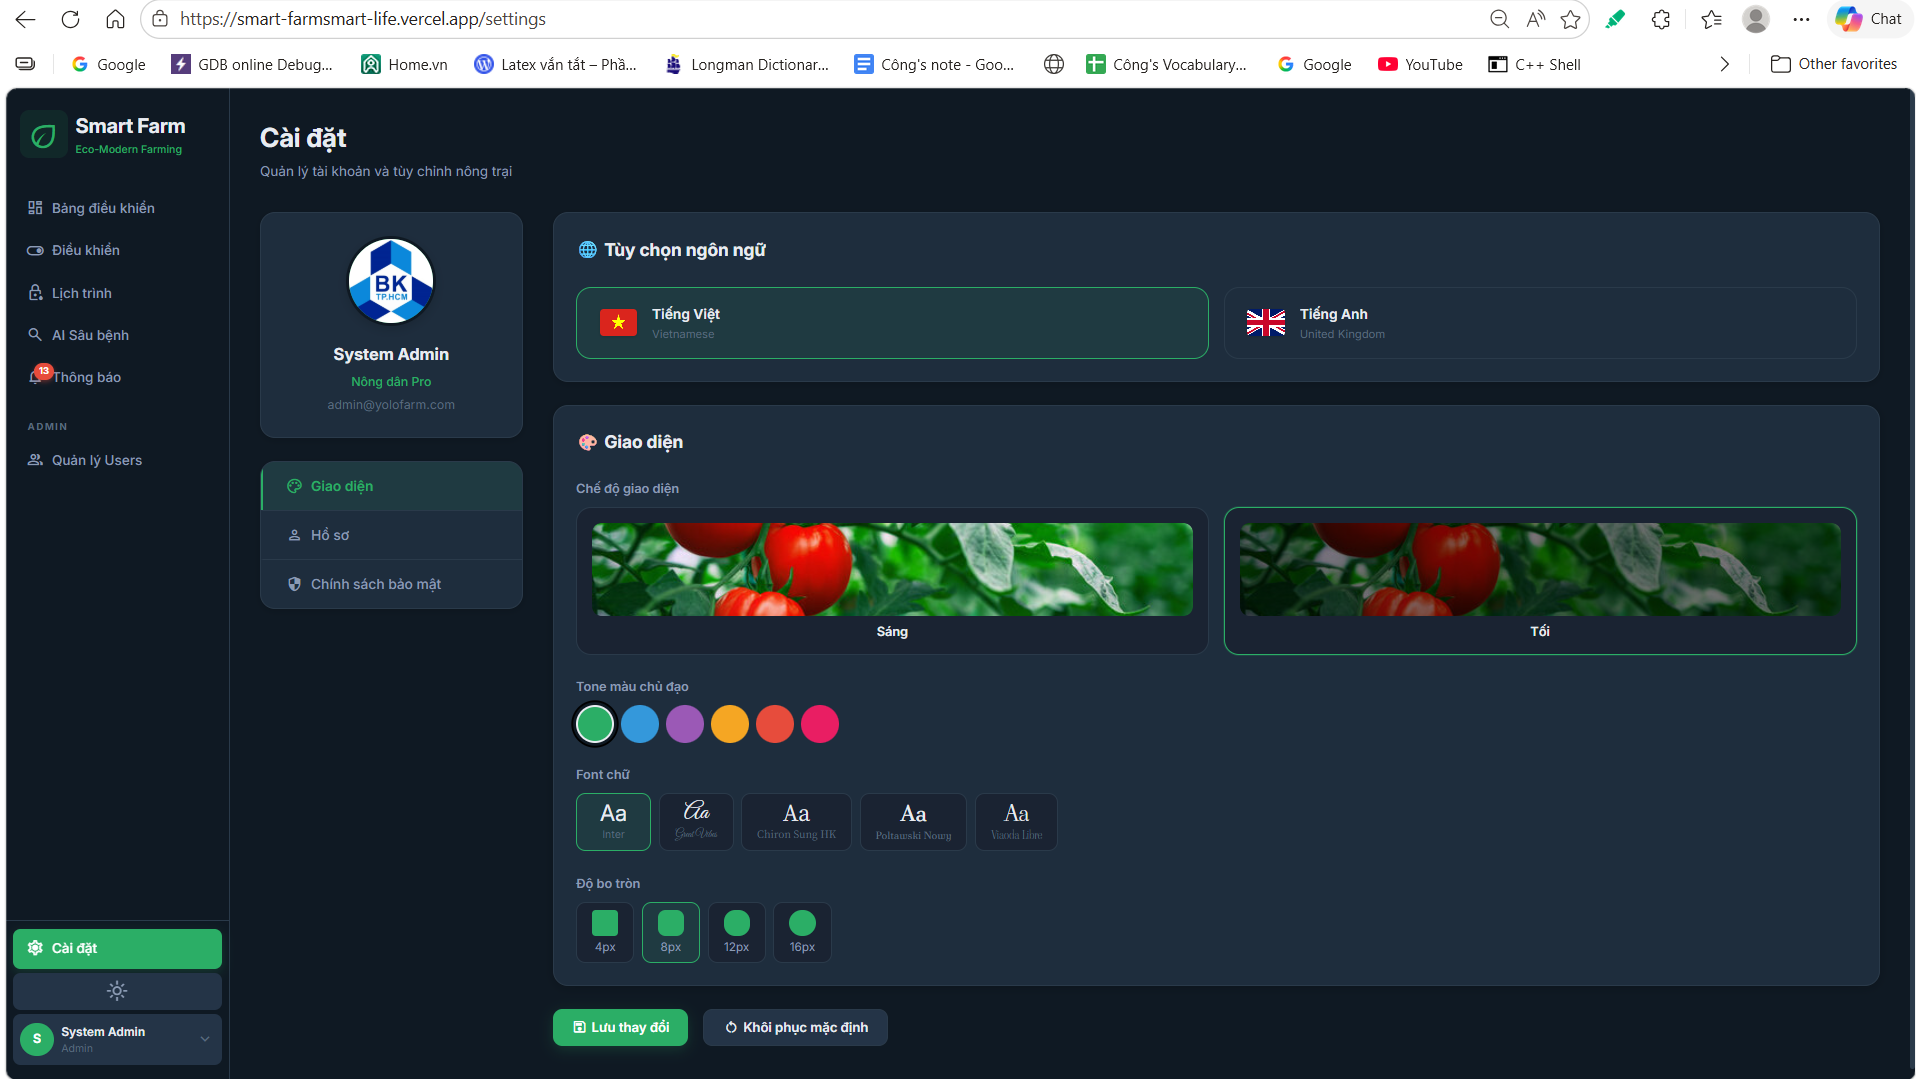
\includegraphics[width=0.85\linewidth]{./Pictures/Task_5/setting_preference.png}
		\caption{Tùy chỉnh giao diện trang web}
	\end{figure}
	
	\item \textbf{Xem hồ sơ của bản thân:} Nơi người dùng có thể cập nhật thông tin cá nhân bao gồm thay đổi tên hiển thị, thay đổi mật khẩu. Cụ thể, việc đổi mật khẩu chỉ có thể được thực hiện bởi người dùng đăng nhập vào hệ thống trực tiếp thay vì đăng nhập bằng tài khoản Google. Nếu đăng nhập bằng tài khoản Google thì người dùng đó không thể điều chỉnh được mật khẩu Google của mình qua trang web này. Đặc biệt, người dùng có thể tải lên ảnh đại diện (avatar) cá nhân, hệ thống sẽ sử dụng dịch vụ Cloudinary để lưu trữ ảnh an toàn.
	\begin{figure}[H]
		\centering
		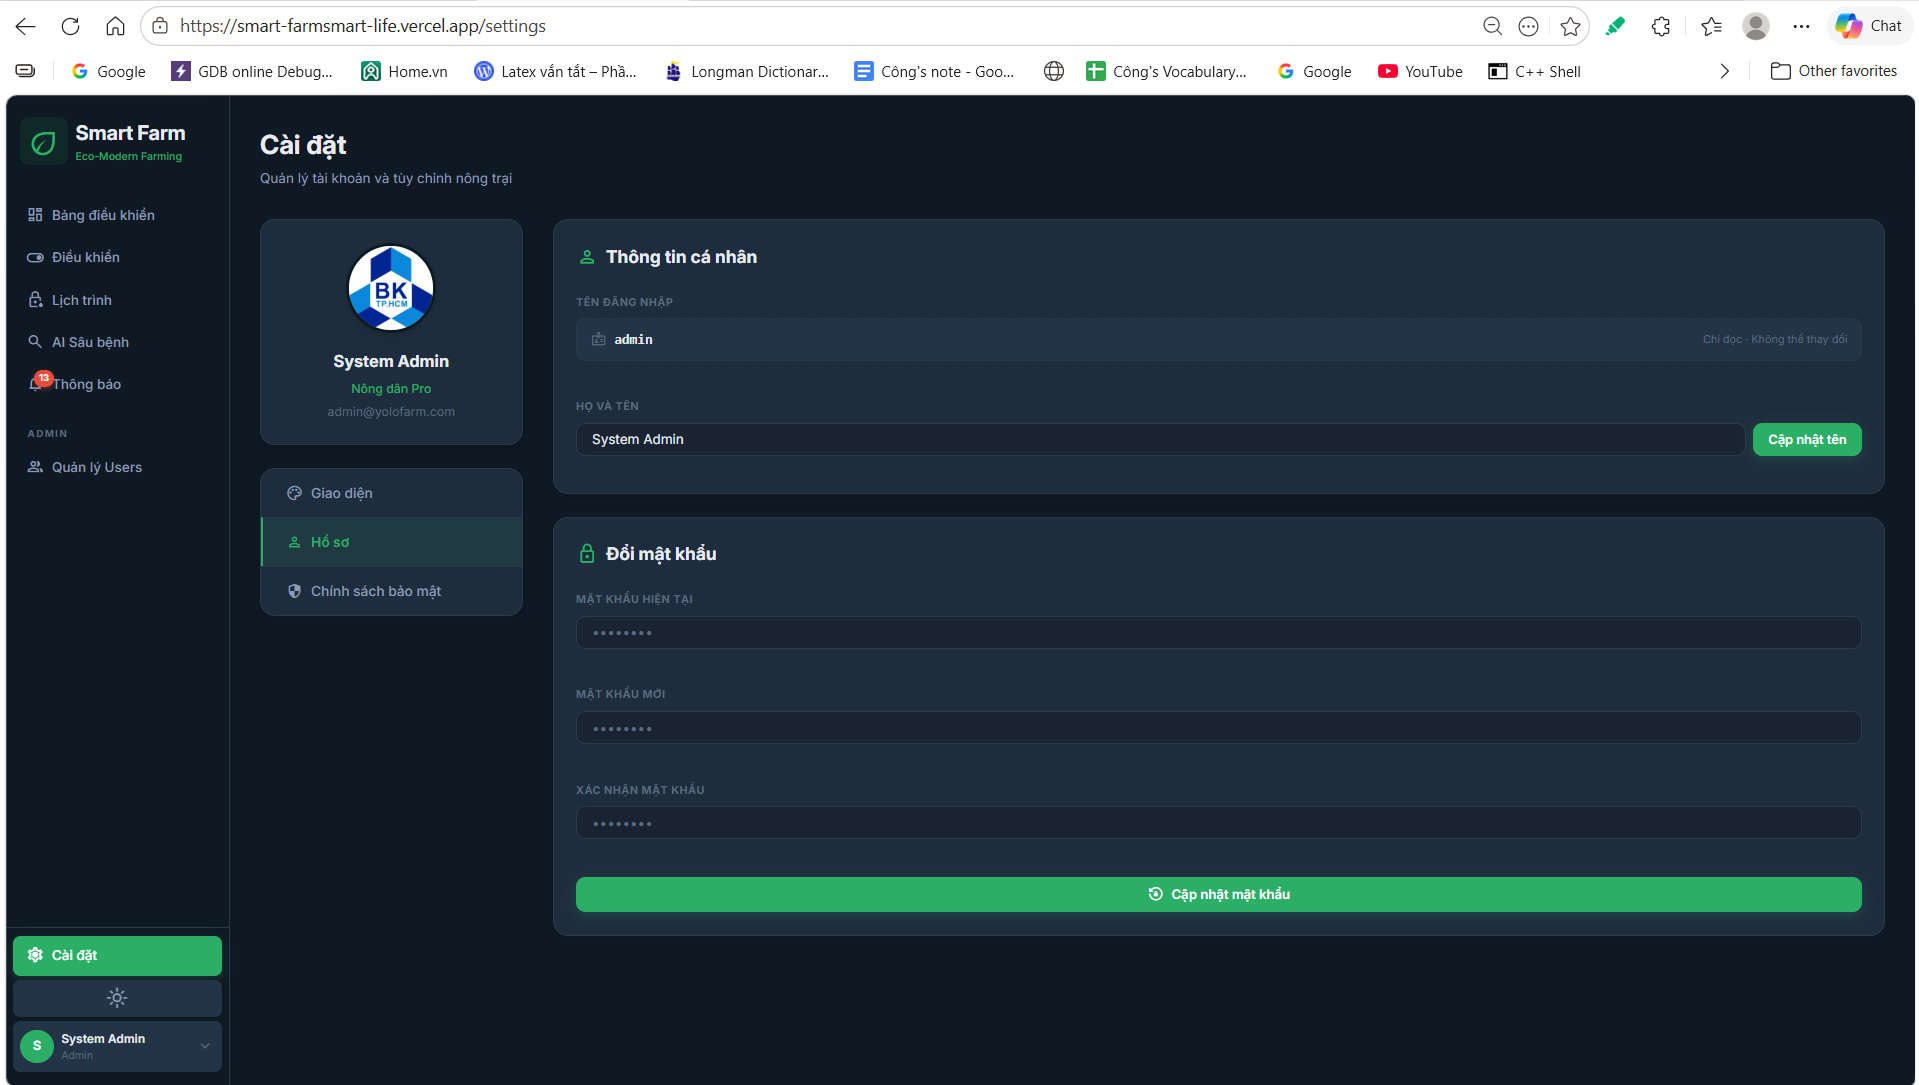
\includegraphics[width=0.85\linewidth]{./Pictures/Task_5/setting_profile.png}
		\caption{Quản lý hồ sơ cá nhân}
	\end{figure}
	
	\item \textbf{Xem chính sách bảo mật của hệ thống:} Hiển thị rõ ràng các quy định sử dụng và chính sách bảo vệ dữ liệu theo dạng Markdown preview.
	\begin{figure}[H]
		\centering
		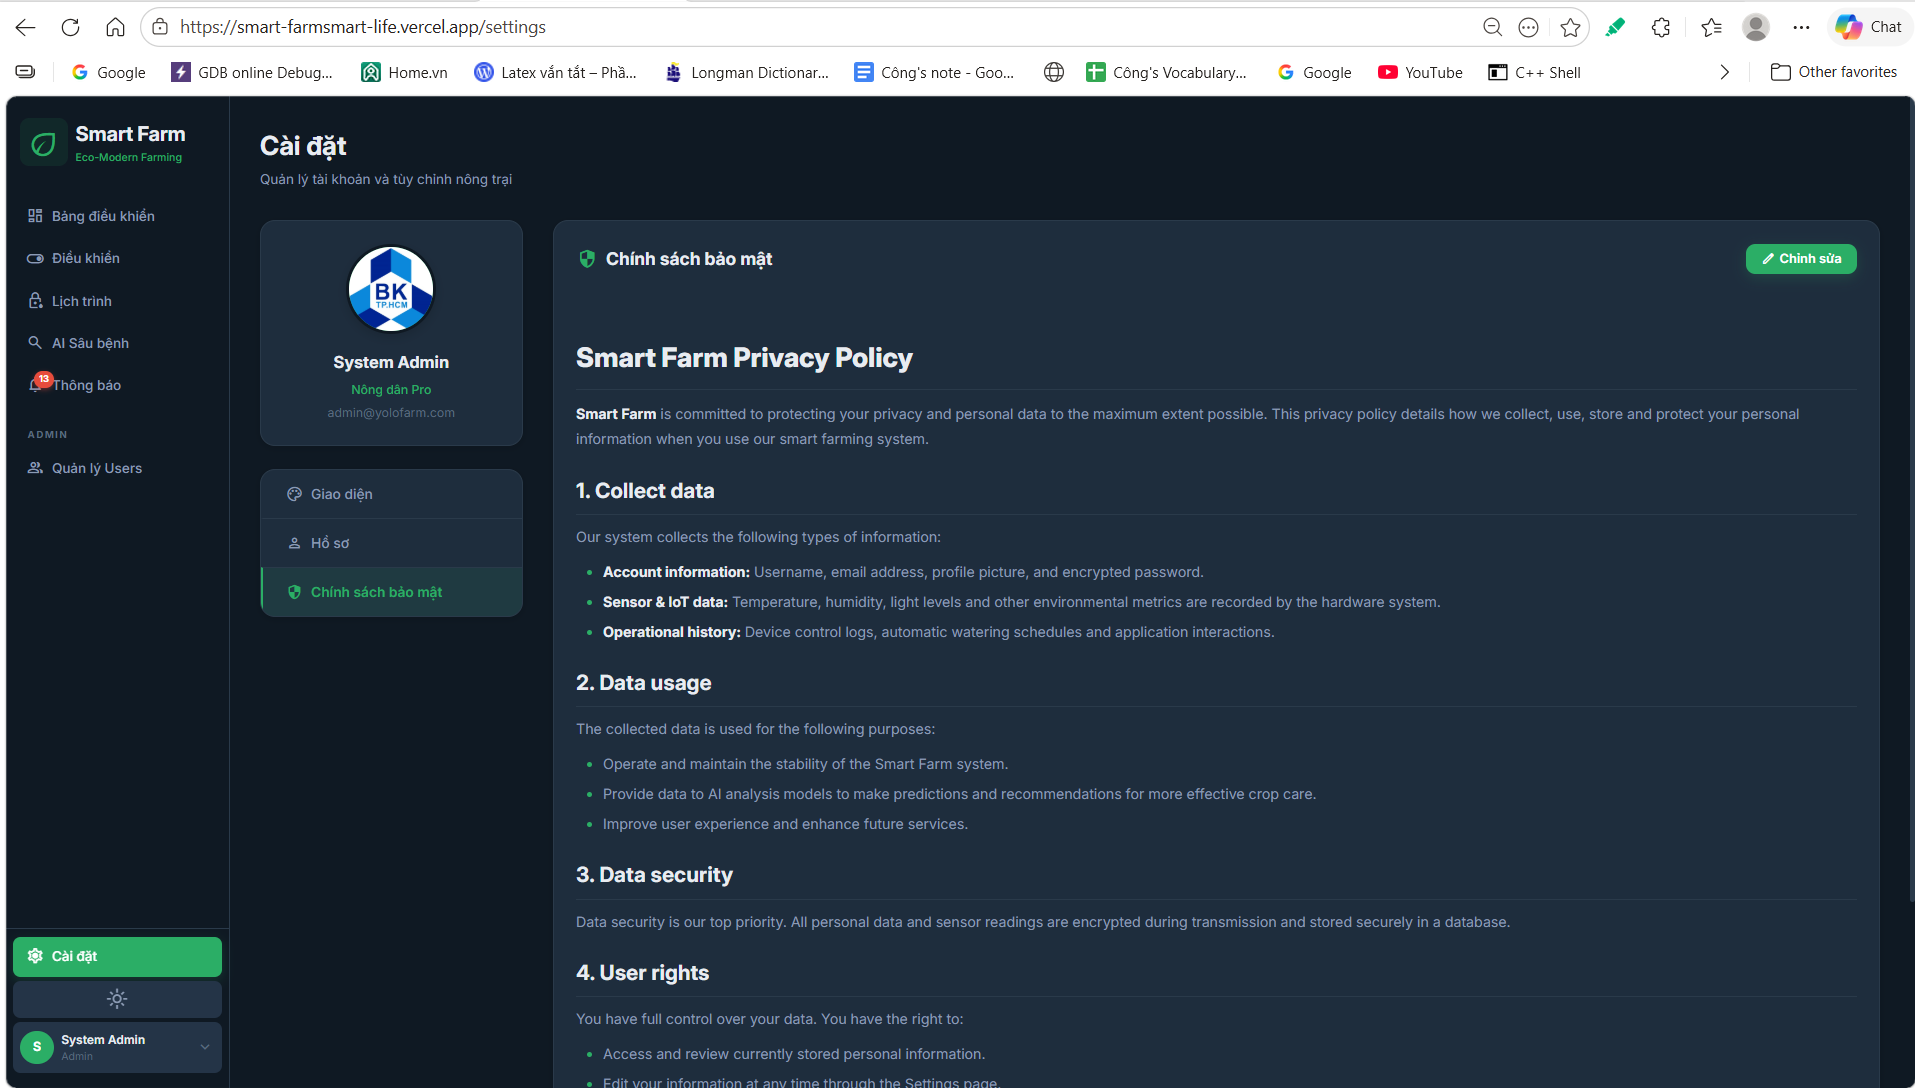
\includegraphics[width=0.85\linewidth]{./Pictures/Task_5/setting_policy.png}
		\caption{Giao diện hiển thị Chính sách bảo mật}
	\end{figure}
	
	\item \textbf{Admin tạo chính sách bảo mật:} Chức năng đặc quyền dành riêng cho quản trị viên (Admin). Admin có thể thêm, chỉnh sửa hoặc xóa nội dung các chính sách của website một cách trực tiếp từ giao diện văn bản bằng cách sử dụng định dạng markdown.
	\begin{figure}[H]
		\centering
		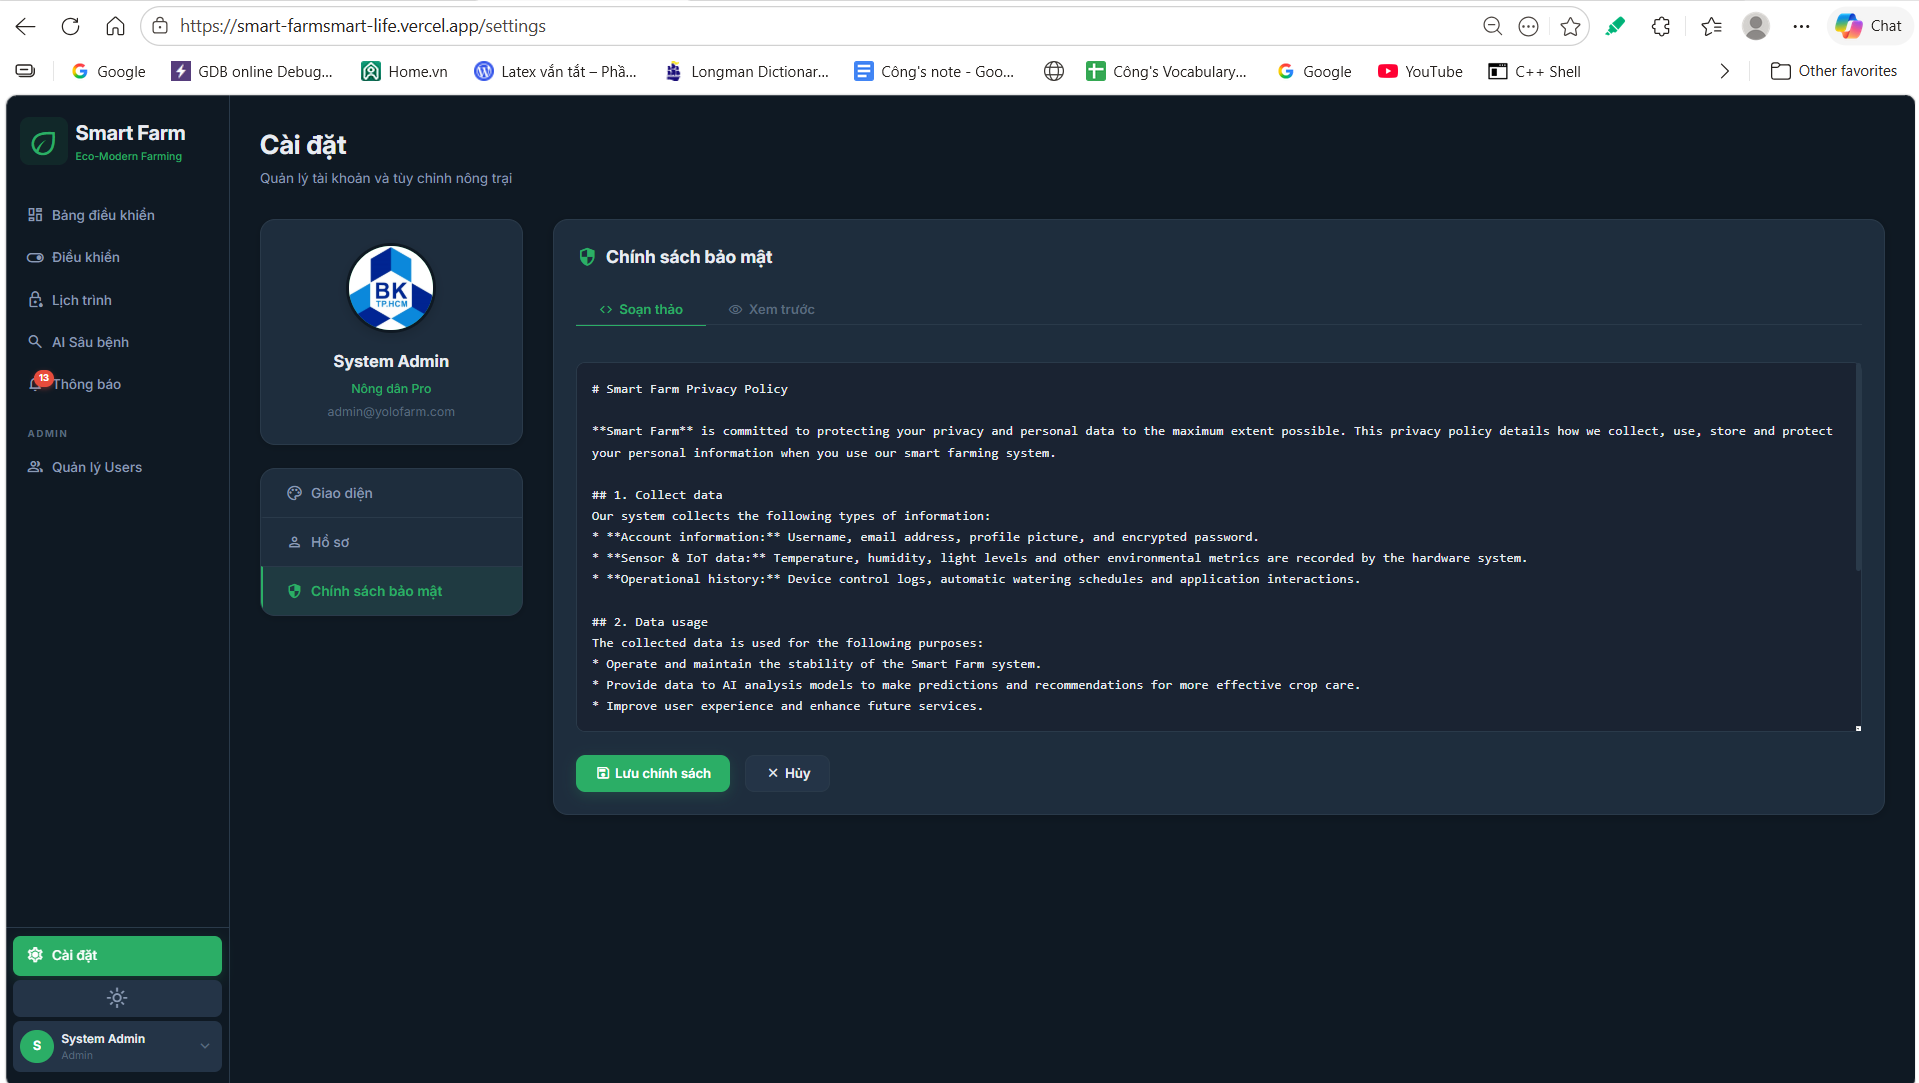
\includegraphics[width=0.85\linewidth]{./Pictures/Task_5/setting_policy_admin.png}
		\caption{Giao diện quản lý Chính sách bảo mật cho quản trị viên}
	\end{figure}

	\item \textbf{Quản lý người dùng (Dành cho Admin):} Phân quyền quản trị cho phép Admin xem danh sách tất cả tài khoản, thực hiện các thao tác cấm (ban) hoặc bỏ cấm (unban) những người dùng có hành vi sai phạm. Ngoài ra cũng có thể thay đổi mật khẩu của một tài khoản user bất kỳ. Khi thay đổi mật khẩu của một người dùng thì hệ thống sẽ gửi mật khẩu mới cho người dùng đó thông qua mục thông báo. Mặt khác, admin cũng có thể thay đổi vai trò của các người dùng khác thành admin hoặc ngược lại.
	\begin{figure}[H]
		\centering
		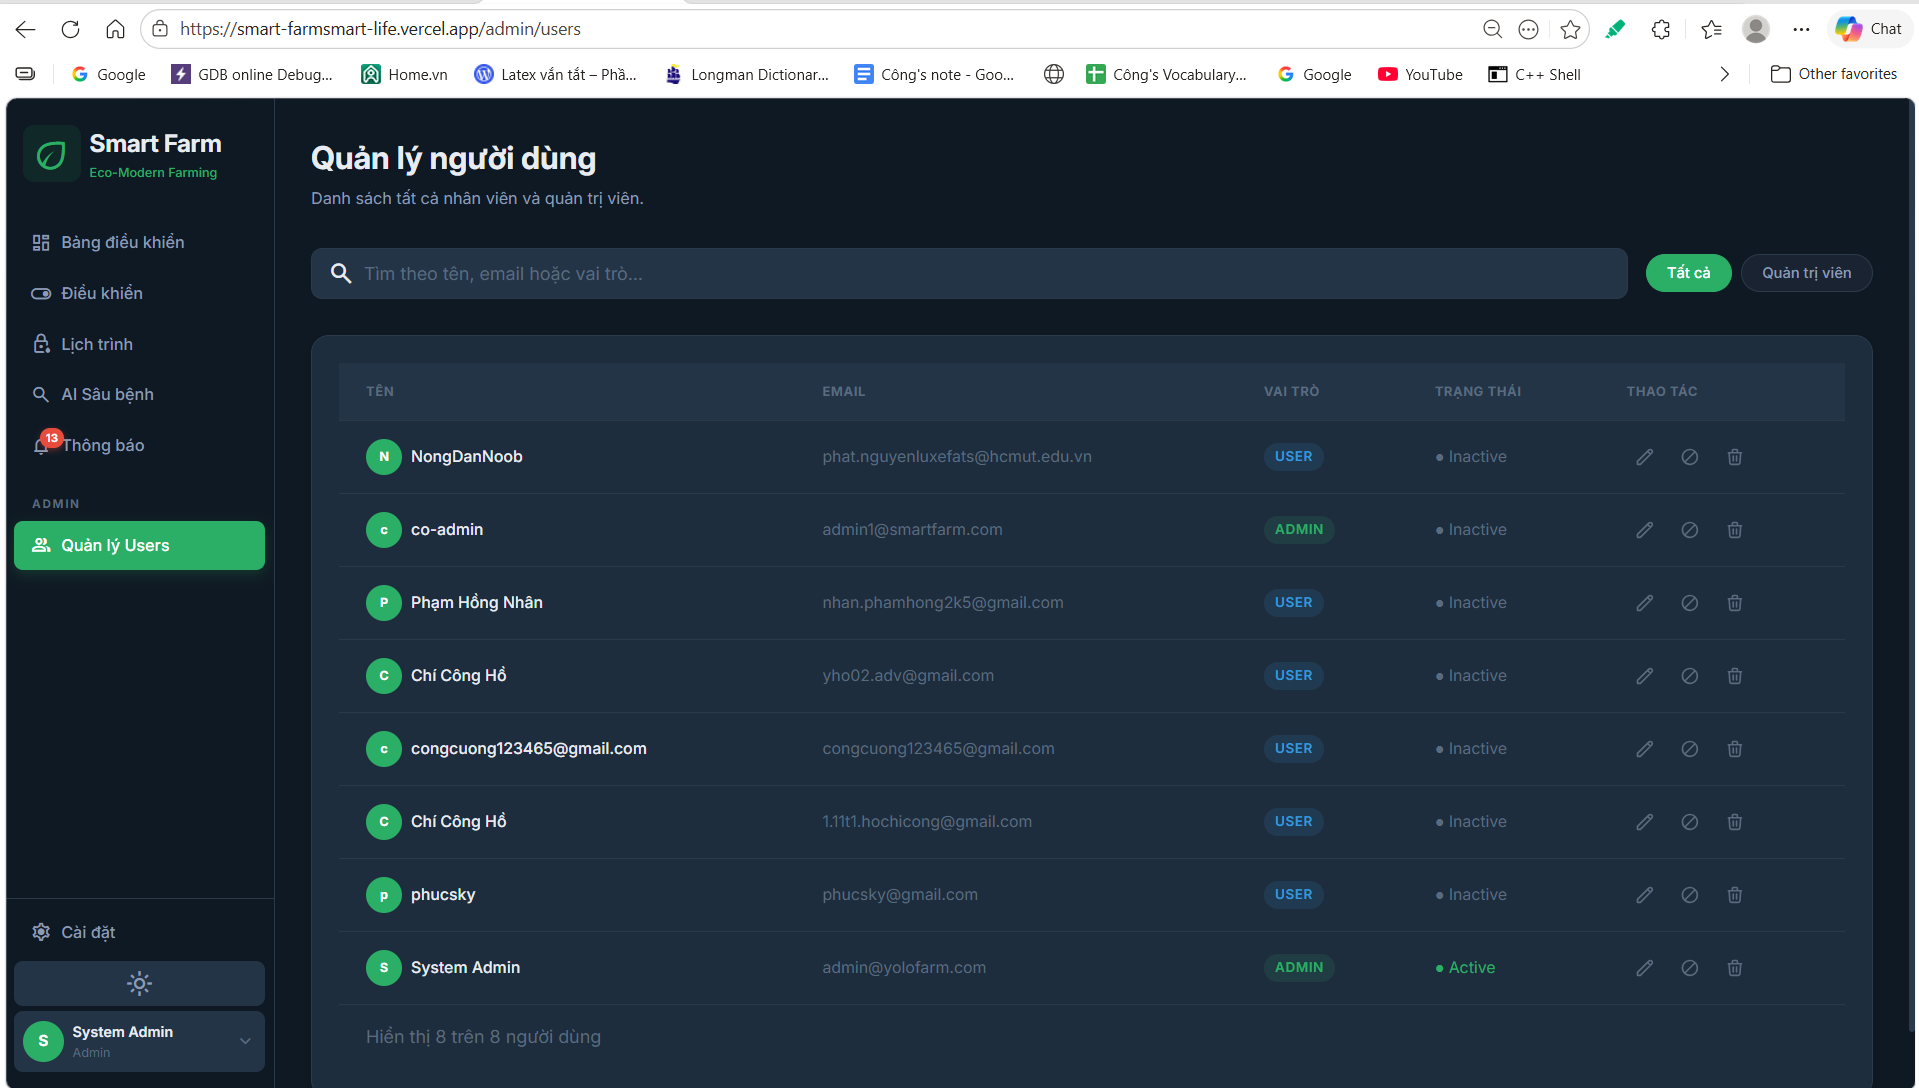
\includegraphics[width=0.85\linewidth]{./Pictures/Task_5/admin_manage_user.png}
		\caption{Danh sách Quản lý người dùng tập trung của Admin}
	\end{figure}
\end{enumerate}
\subsubsection{Giao diện Dashboard}
\indent Phần giao diện tổng quan của hệ thống gồm có 3 phần chính:
\begin{enumerate}[label=\arabic*., leftmargin=1.5cm]
    \item Phần xem nhiệt độ, độ ẩm, độ ẩm đất: Thông tin của các cảm biến được hiển thị dưới dạng số liệu được lấy từ adafruit-io. Số liệu được đưa lên adafruit chính là số liệu thật của các cảm biến tương ứng trả về. Cụ thể hơn, nếu chưa có phần cứng trực tiếp kết nối với adafruit thì hệ thống sẽ gọi API tới open-meteo để lấy dữ liệu thời tiết thật tại tọa độ xác định và gửi dữ liệu lên Adafruit. Đảm bảo rằng dữ liệu luôn được cập nhật một cách chính xác.
    \item Phần điều khiển thiết bị: Người dùng có thể điều khiển các thiết bị như hai máy bơm nước và đèn LED từ xa (có thể điều khiển từ các thiết bị khác nhau) nhờ việc đã kết nối hệ thống phần mềm với Adafruit và đồng thời kết nối Adafruit với hệ thống phần cứng. Điều này cho phép rằng, một khi phần mềm được deploy thành công, tức có nhiều người dùng truy cập vào hệ thống cùng một lúc thì có thể cùng điều khiển các thiết bị có trong nông trại.
    \item Phần biểu đồ miền hiển thị thông tin lịch sử nhiệt độ, độ ẩm, độ ẩm đất và cường độ ánh sáng mà các cảm biến ghi nhận được trong một ngày. Cụ thể, hệ thống sẽ lấy dữ liệu trực tiếp tại adafruit, tổng hợp lại và vẽ điểm tương ứng ra phần biểu đồ miền này. Từ đó giúp cho việc huấn luyện mô hình dự đoán xu hướng thời tiết, độ ẩm, cường độ ánh sáng và giúp xác định loại bệnh của lá cây một cách dễ dàng hơn.
\end{enumerate}
\begin{figure}[H]
	\centering
	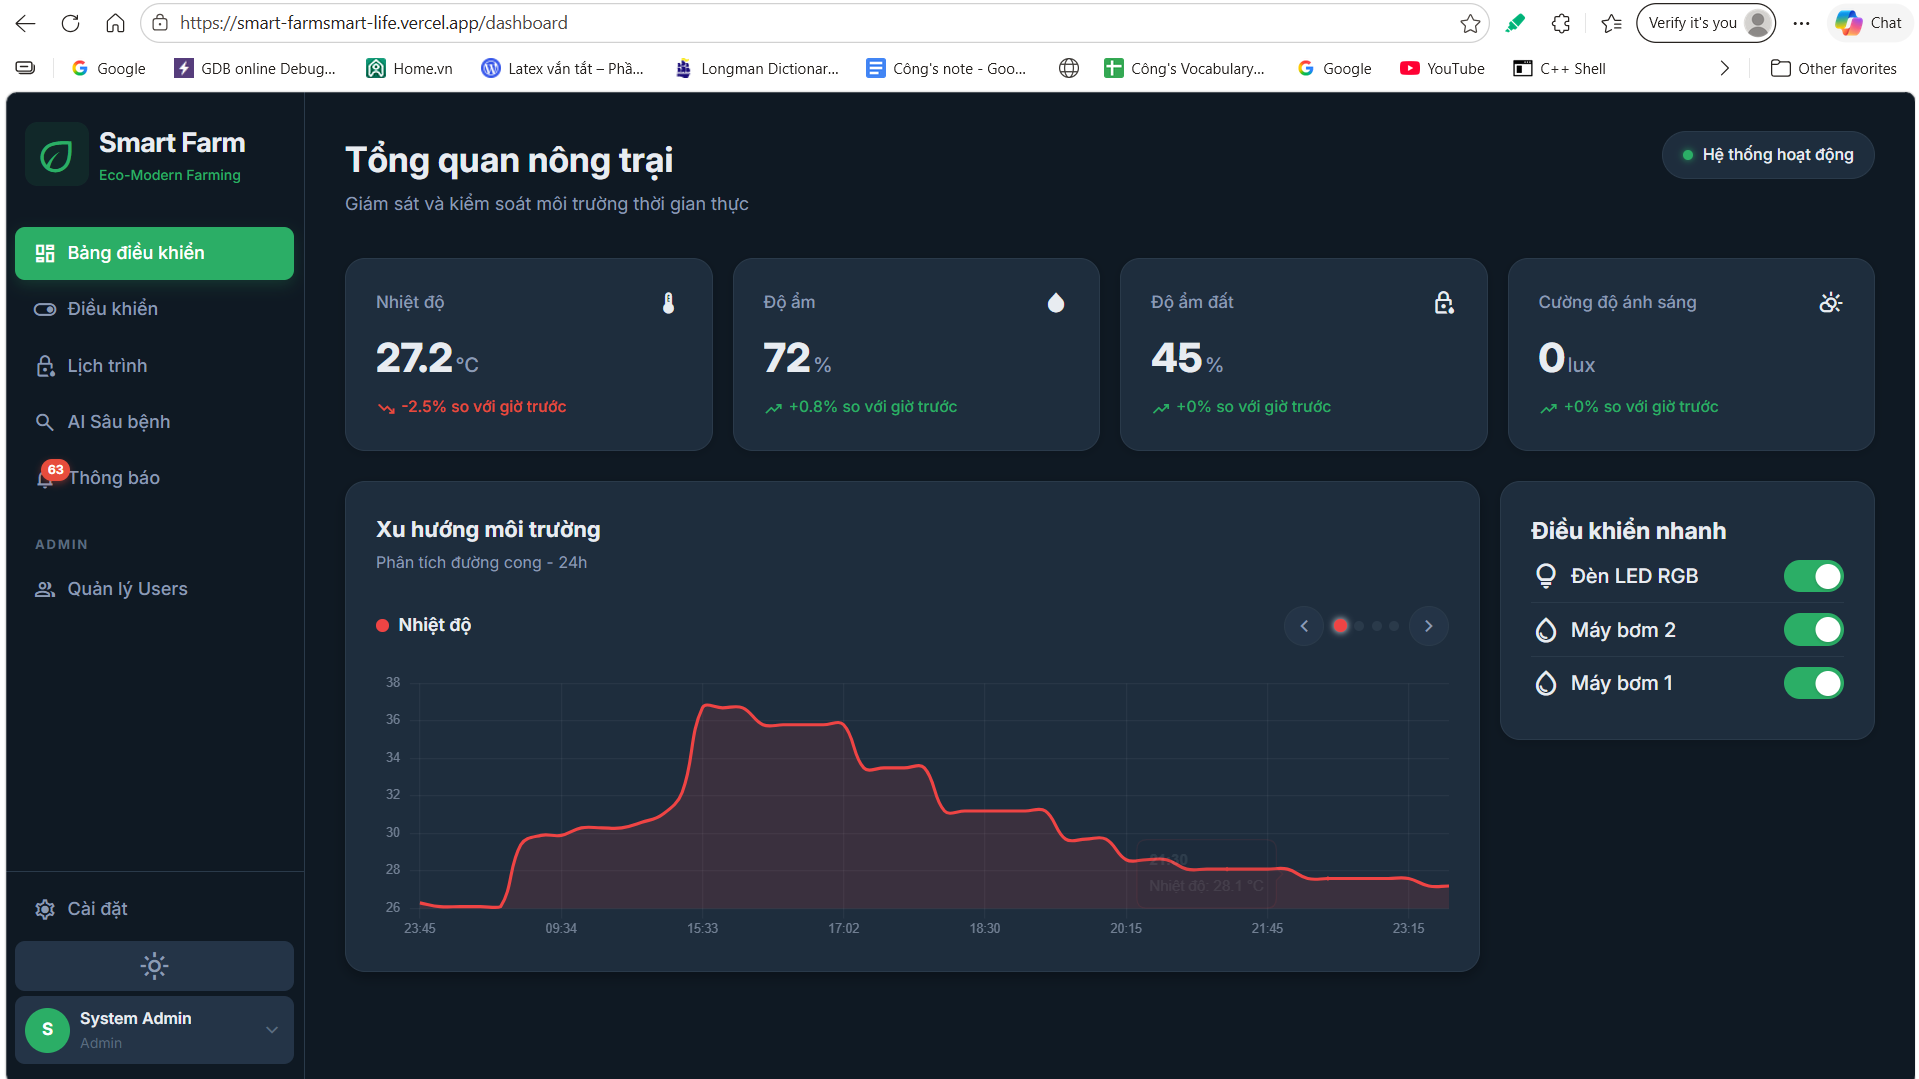
\includegraphics[width=0.8\linewidth]{./Pictures/Task_5/overview.png}
	\caption{Tổng quan hệ thống}
\end{figure}
\subsubsection{Giao diện điều khiển}
\indent Giao diện điều khiển là nơi cho phép người dùng quản lý trọn vẹn tất cả thiết bị được kết nối. Khi người dùng thao tác tương tác bằng cách bật/tắt thiết bị tại đây, tín hiệu sẽ đi qua backend API viết trên Node.js và nhanh chóng giao tiếp với Adafruit IO trực tiếp thông qua giao thức MQTT.\\
\indent Hệ thống hỗ trợ xử lý nhiều thiết bị cùng lúc (ví dụ như hai máy bơm \texttt{pump1}, \texttt{pump2} và một đèn \texttt{led-rgb}). Các trạng thái đang hoạt động, khu vực được phân bổ, chức năng, và thời gian hoạt động của máy bơm nước hay đèn chiếu sáng đều được phản hồi theo thời gian thực (realtime) lên phần mềm. Điều này có nghĩa là cho dù thiết bị được bật, tắt từ web app, hay từ mạng phần cứng, trạng thái đều đồng bộ cả hai chiều, giúp người dùng dễ quản lý và hạn chế rủi ro cho trang trại.
\begin{figure}[H]
	\centering
	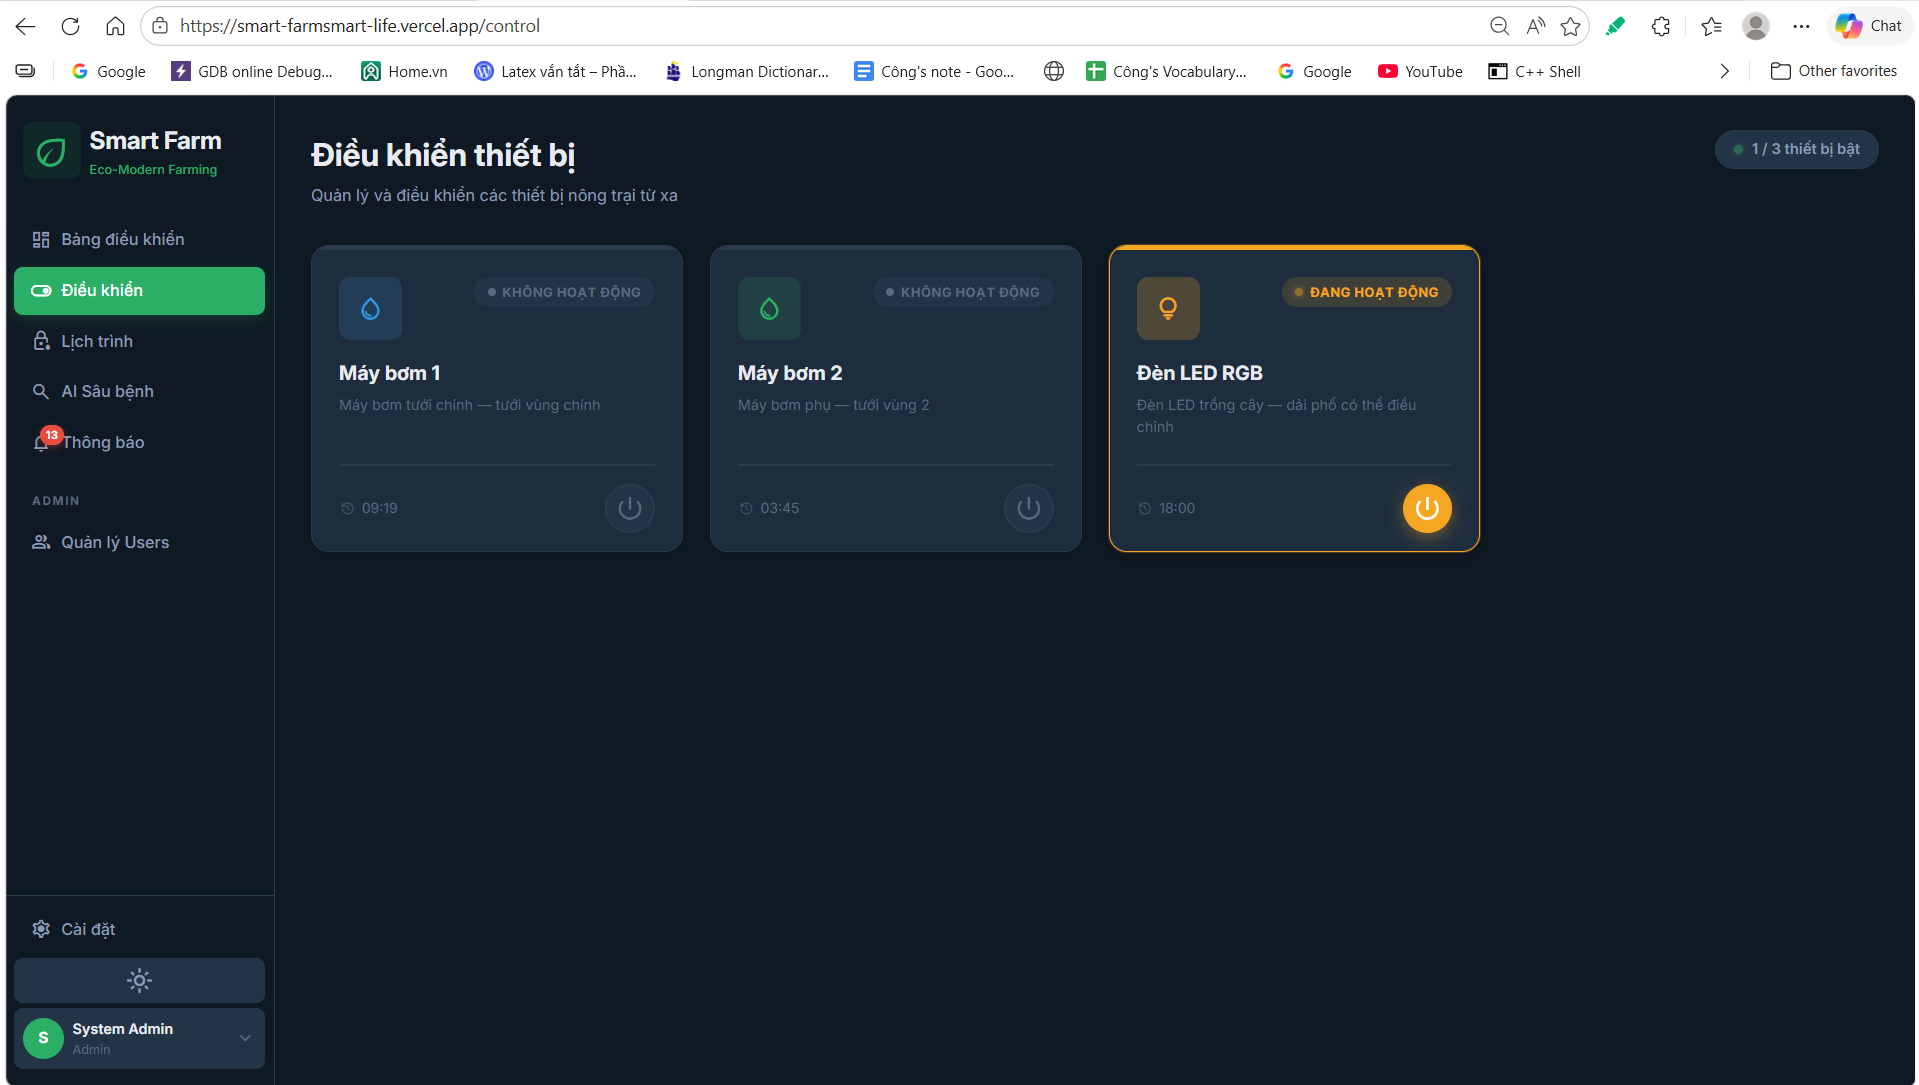
\includegraphics[width=0.8\linewidth]{./Pictures/Task_5/control_panel.png}
	\caption{Giao diện bảng điều khiển thiết bị (Control Panel)}
\end{figure}

\subsubsection{Giao diện phần lịch trình}
\indent Phần này cho phép người dùng thiết lập và xem được phần lịch trình đã được lên sẵn để điều khiển các thiết bị có trong trang trại. Cụ thể, người dùng có thể xem được tất cả các khung giờ mà tất cả người dùng của trang trại đã đặt để điều khiển các thiết bị tương ứng. Ví dụ, người dùng A có thể xem được lịch mà các người dùng khác (giả sử là B và Admin) đã thiết lập để hệ thống bật/tắt thiết bị (đèn chiếu sáng) một cách tự động.\\
\indent Nếu đăng nhập với vai trò là ``người dùng'' thì chỉ có thể điều chỉnh lịch trình của chính mình. Mặt khác, nếu có vai trò là ``admin'' thì có thể xóa lịch trình của những người khác.

\begin{figure}[H]
	\centering
	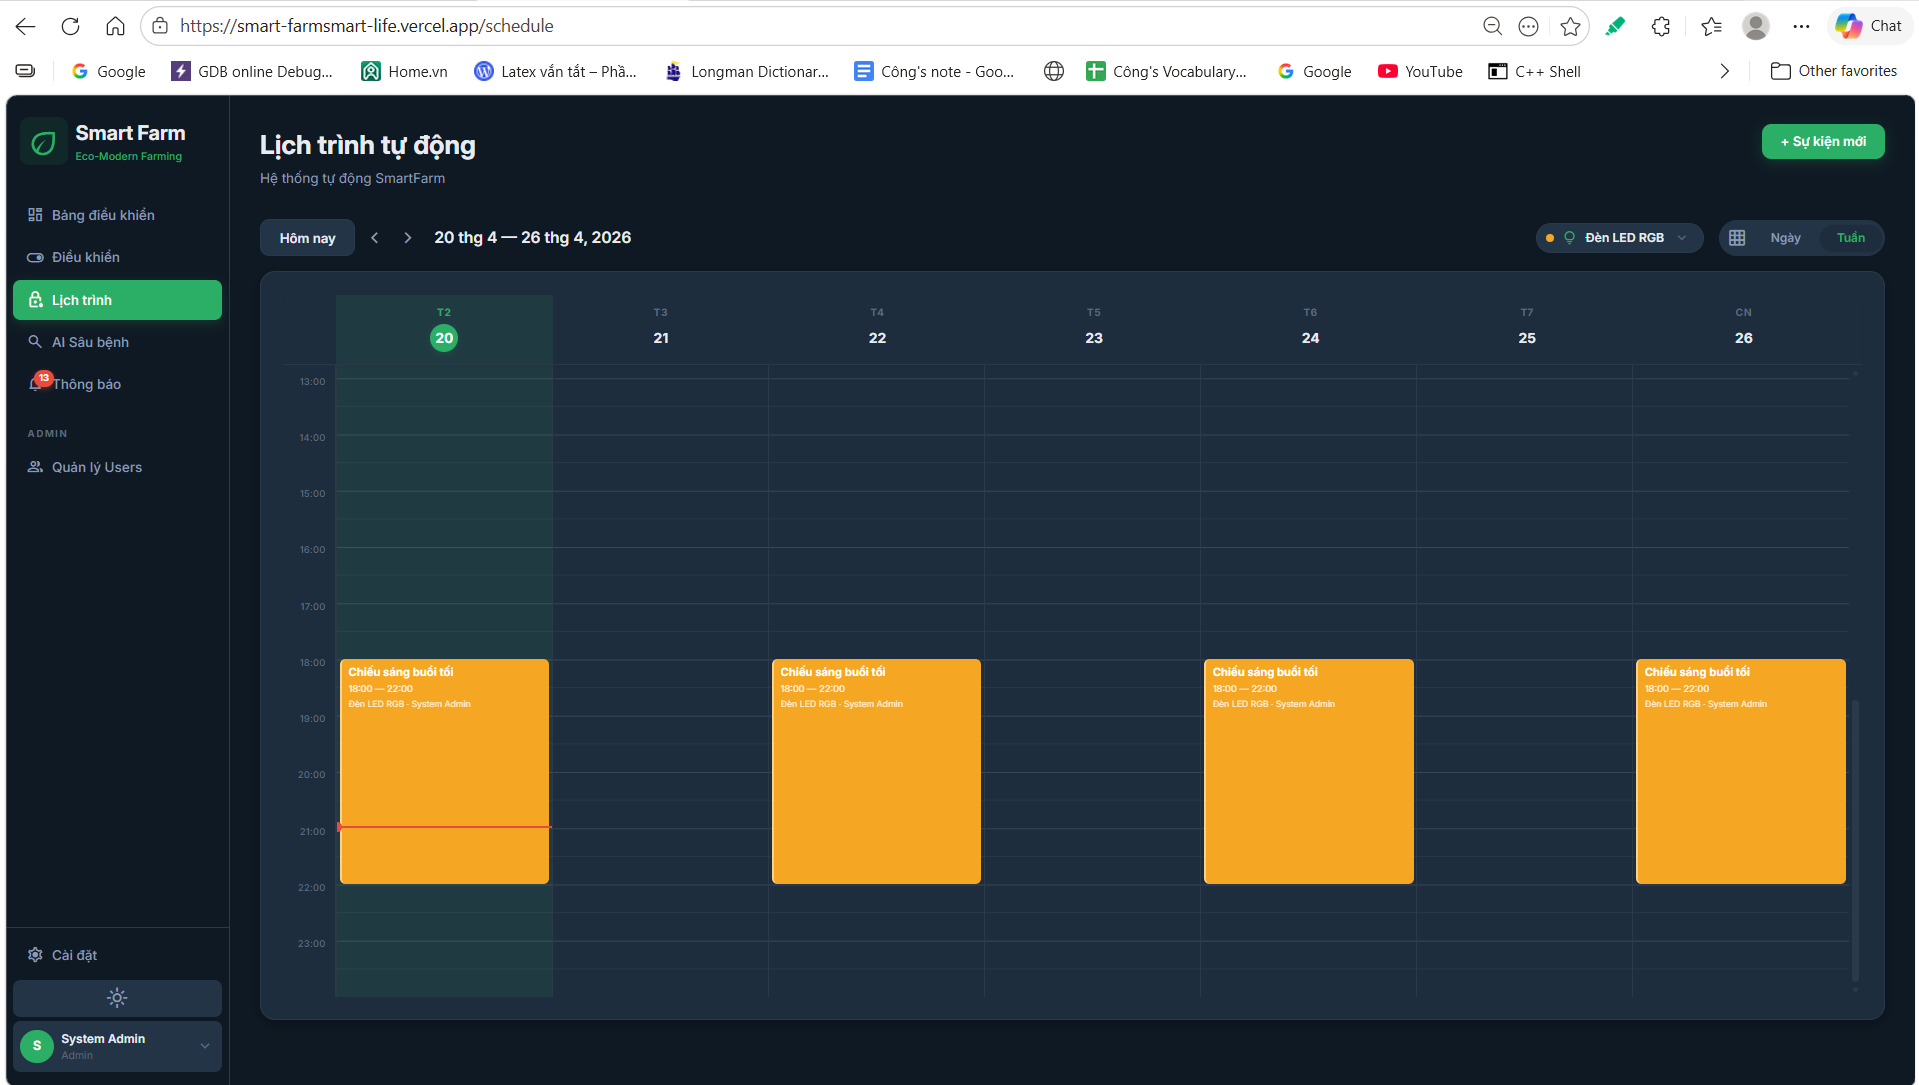
\includegraphics[width=0.8\linewidth]{./Pictures/Task_5/schedule.png}
	\caption{Giao diện phần xem lịch trình tự động hóa}
\end{figure}
\indent Có thể xem được lịch trình theo nhiều chế độ. Cụ thể là theo ngày hoặc theo tuần trên một timeline dựa vào thời gian thực. Ngoài ra, người dùng còn có thể chọn các thiết bị cần xem lịch trình (máy bơm 1, 2 hoặc đèn LED).\\
\indent Mặt khác, có thể thêm lịch trình mới bằng cách nhấn vào nút ``Sự kiện mới'' ở góc trên bên phải màn hình. Khi bấm vào nút này thì một cửa sổ nhỏ hiện lên với các thông tin mà người dùng cần phải điền để có thể thêm một lịch trình mới cho một trong các thiết bị một cách hợp lệ. Nếu lịch được thêm có ngày bắt đầu là một thời điểm trong quá khứ so với thời gian thực thì hệ thống sẽ không ghi nhận lịch trình này và báo lỗi ``lịch trình không thể bắt đầu vào một thời điểm trong quá khứ''. Mặt khác, nếu ngày kết thúc nhỏ hơn ngày bắt đầu cũng sẽ có lỗi xảy ra.\\
\indent Khi thời gian thực tới thời điểm bắt đầu một lịch trình nào đó thì hệ thống sẽ kiểm tra xem thiết bị đã hoạt động hay chưa. Nếu chưa thì hệ thống sẽ tự động khởi động (bật) thiết bị đó lên. Khi kết thúc lịch trình, nếu thiết bị đang bật thì hệ thống sẽ tắt thiết bị đó đi một cách hoàn toàn tự động.
\begin{figure}[H]
	\centering
	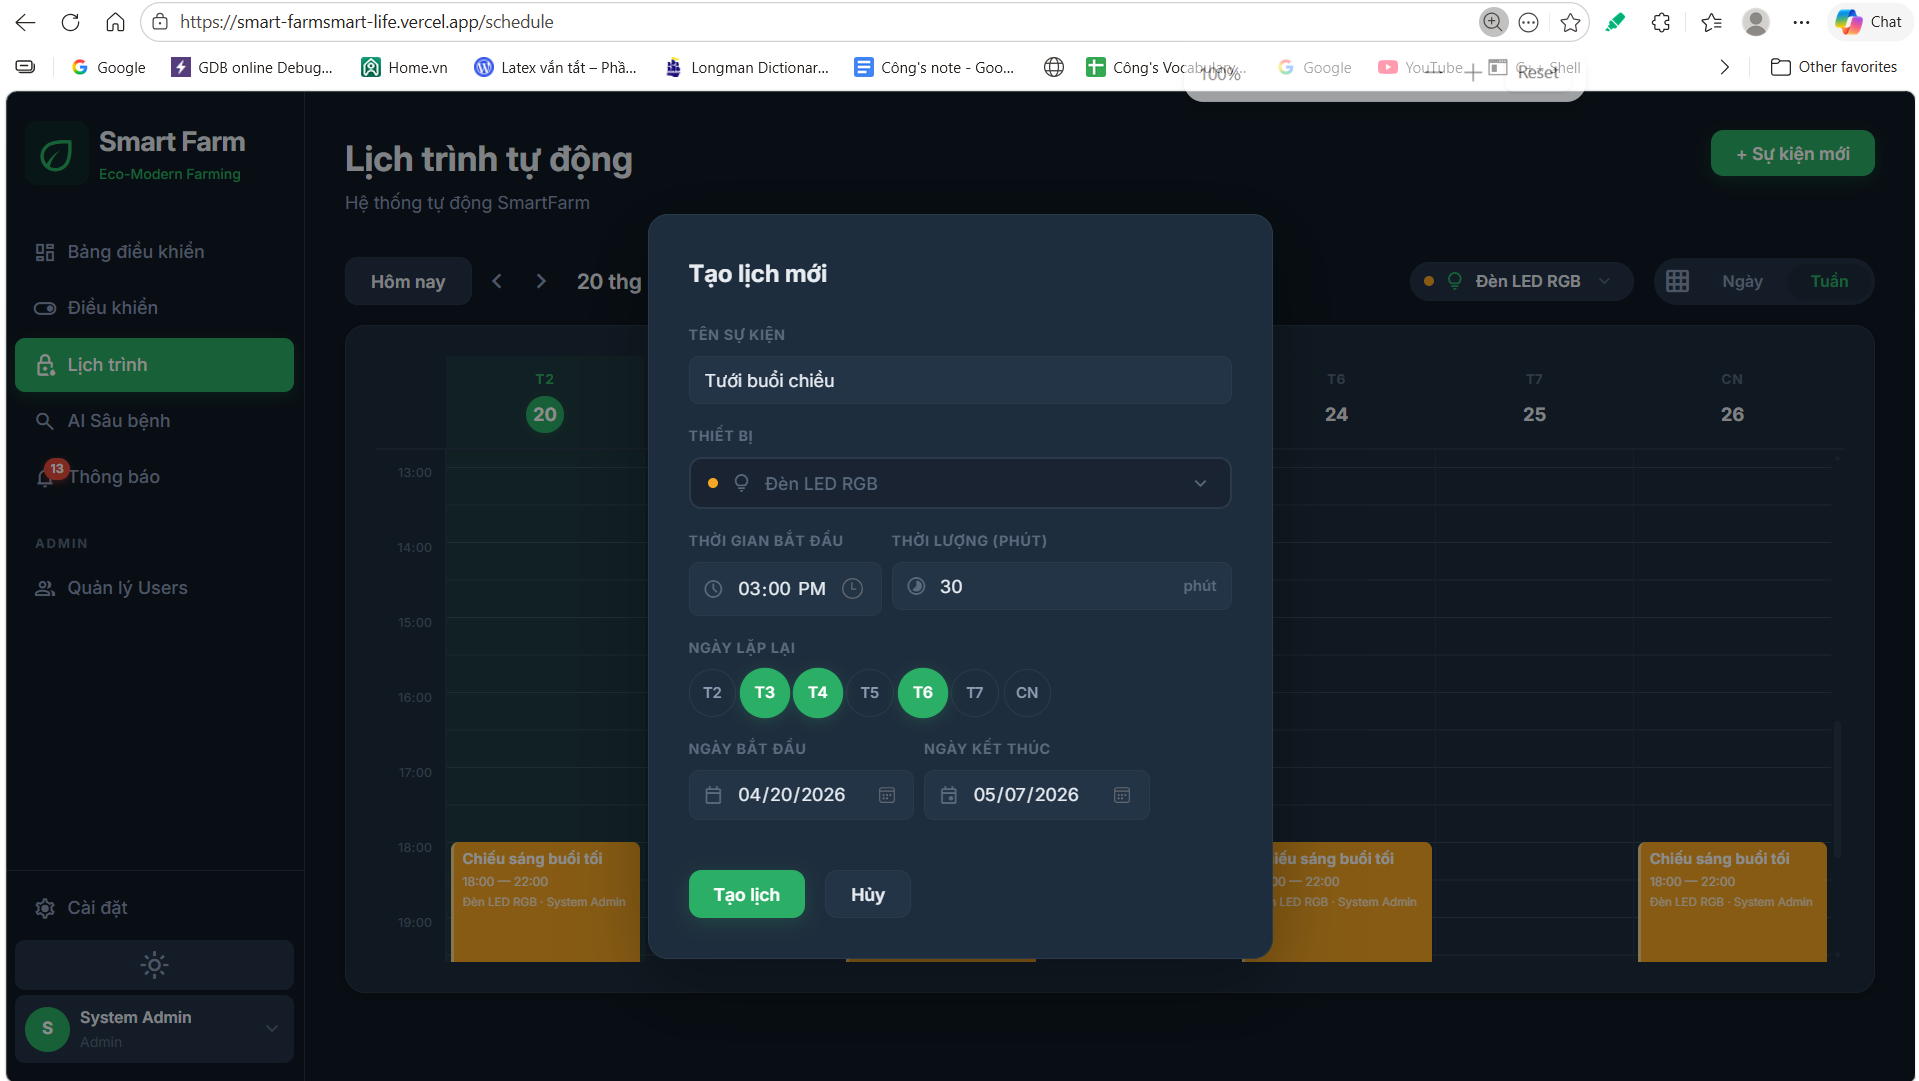
\includegraphics[width=0.8\linewidth]{./Pictures/Task_5/schedule_setup.png}
	\caption{Giao diện phần thêm lịch trình mới}
\end{figure}
\subsubsection{Giao diện hệ thống thông báo}
\indent Giao diện thông báo giúp tổng hợp và cập nhật liên tục cho người dùng nếu có cảnh báo về môi trường (như nhiệt độ bất thường, độ ẩm thấp) hoặc các sự kiện tự động hoá (đã đến giờ bật bơm). Các thông báo này đẩy qua dịch vụ Socket.IO hiển thị tự động. Nhờ giao diện trực quan, người quản trị có thể dễ dàng đánh dấu đã đọc một hay tất cả thông báo, có thể ghim/lưu (save) các cảnh báo trọng điểm, cũng như chọn xóa đi khi không cần thiết.
\begin{figure}[H]
	\centering
	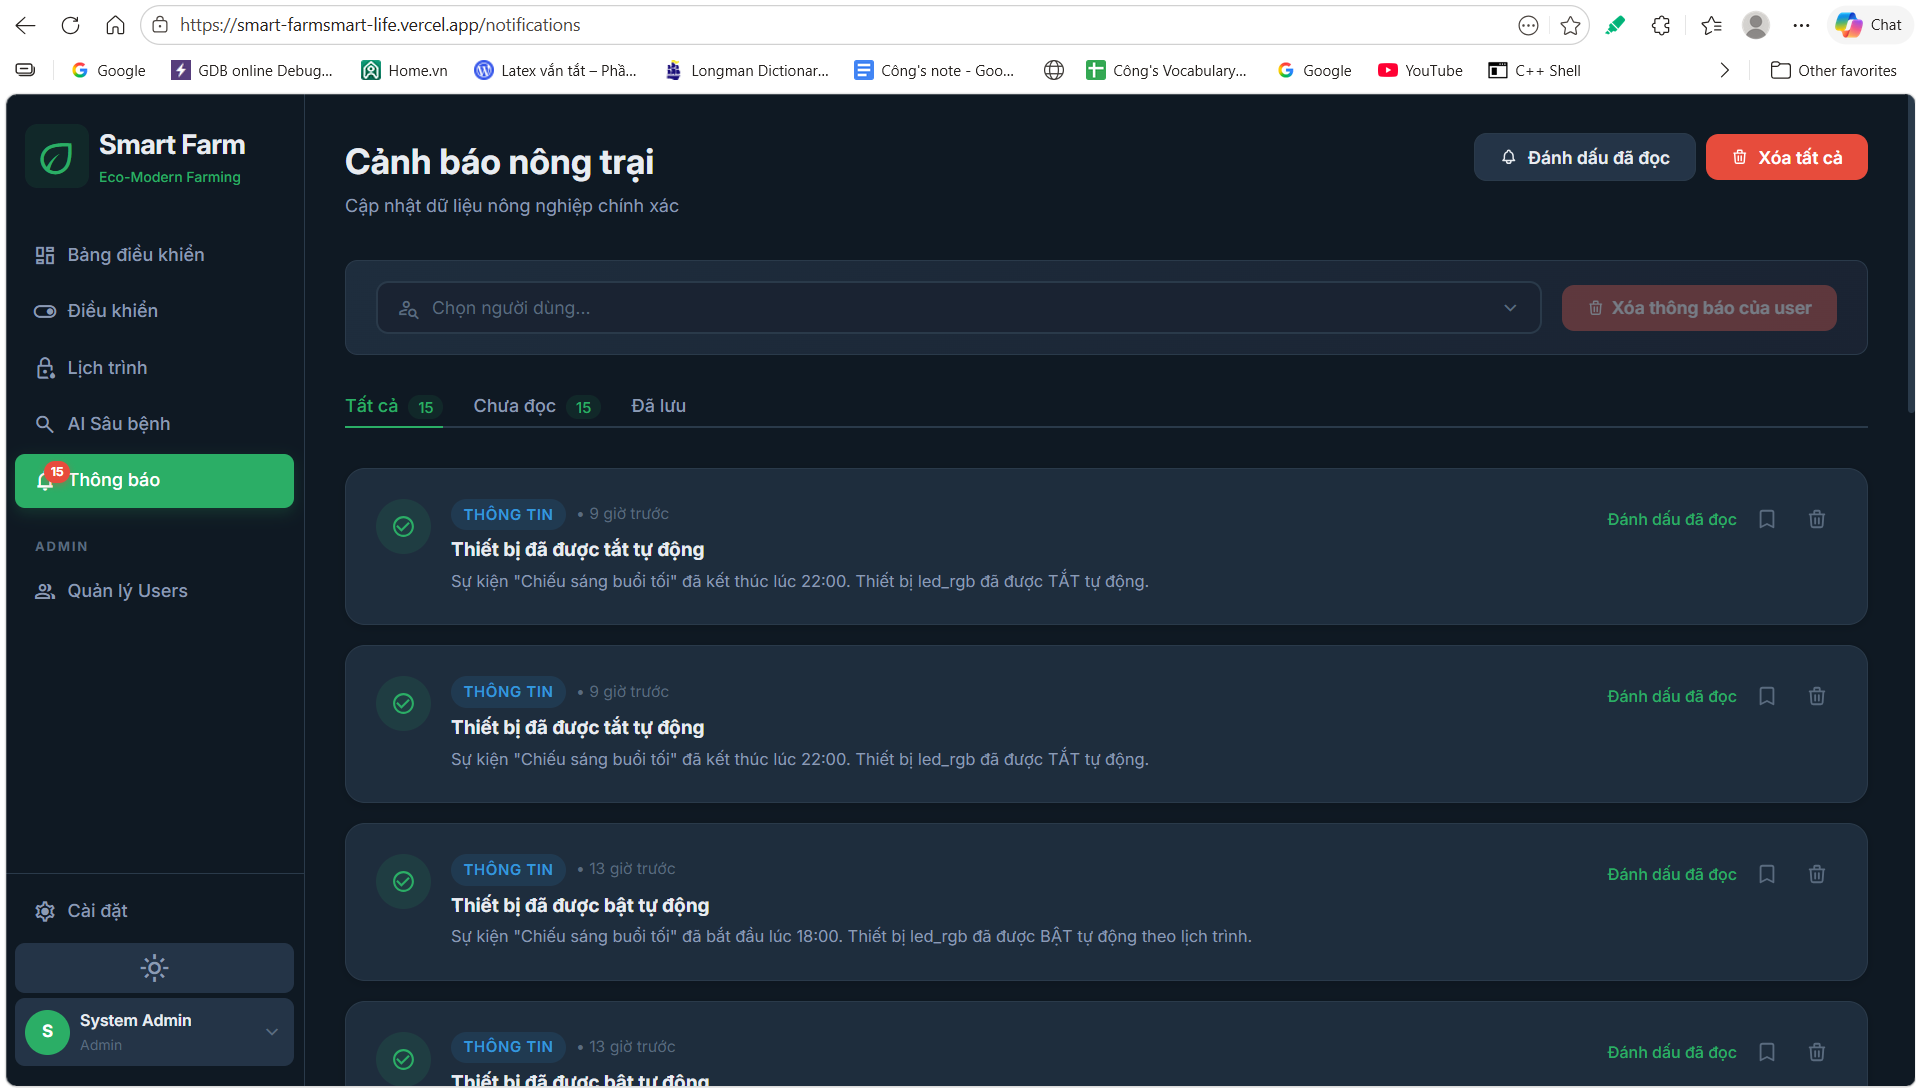
\includegraphics[width=0.9\linewidth]{./Pictures/Task_5/notification.png}
	\caption{Giao diện hệ thống thông báo báo động và giám sát}
\end{figure}

\subsection{Huấn luyện AI nhận diện lá cây bệnh}
\indent Một trong những tính năng nổi bật của SmartFarm là việc tích hợp Trí tuệ nhân tạo (AI) giúp chẩn đoán và phát hiện tình trạng sâu bệnh trên lá cây dựa vào việc phân tích và xử lý các loại hình ảnh của lá cây cà chua (png, jpg, jpeg).\\
\indent Dịch vụ AI này chia thành một microservice hoạt động độc lập bằng FastAPI, sử dụng kiến trúc mạng nơ-ron tích chập nổi bật \textbf{EfficientNet}. Thông qua việc tải ảnh lá cây bệnh lên hệ thống, tiến trình backend tại đây sẽ uỷ thác cho nền tảng AI phân tích. Chỉ trong vài giây, hệ thống trả ra dữ liệu kết quả là Tên loại bệnh, độ tự tin (confidence) của chẩn đoán mô hình, và ngay lập tức cung cấp phác đồ cách thức khắc phục (Ví dụ cắt cành sâu trị nấm,...). Đây là một ưu điểm rất lớn của hệ thống.

\begin{figure}[H]
	\centering
	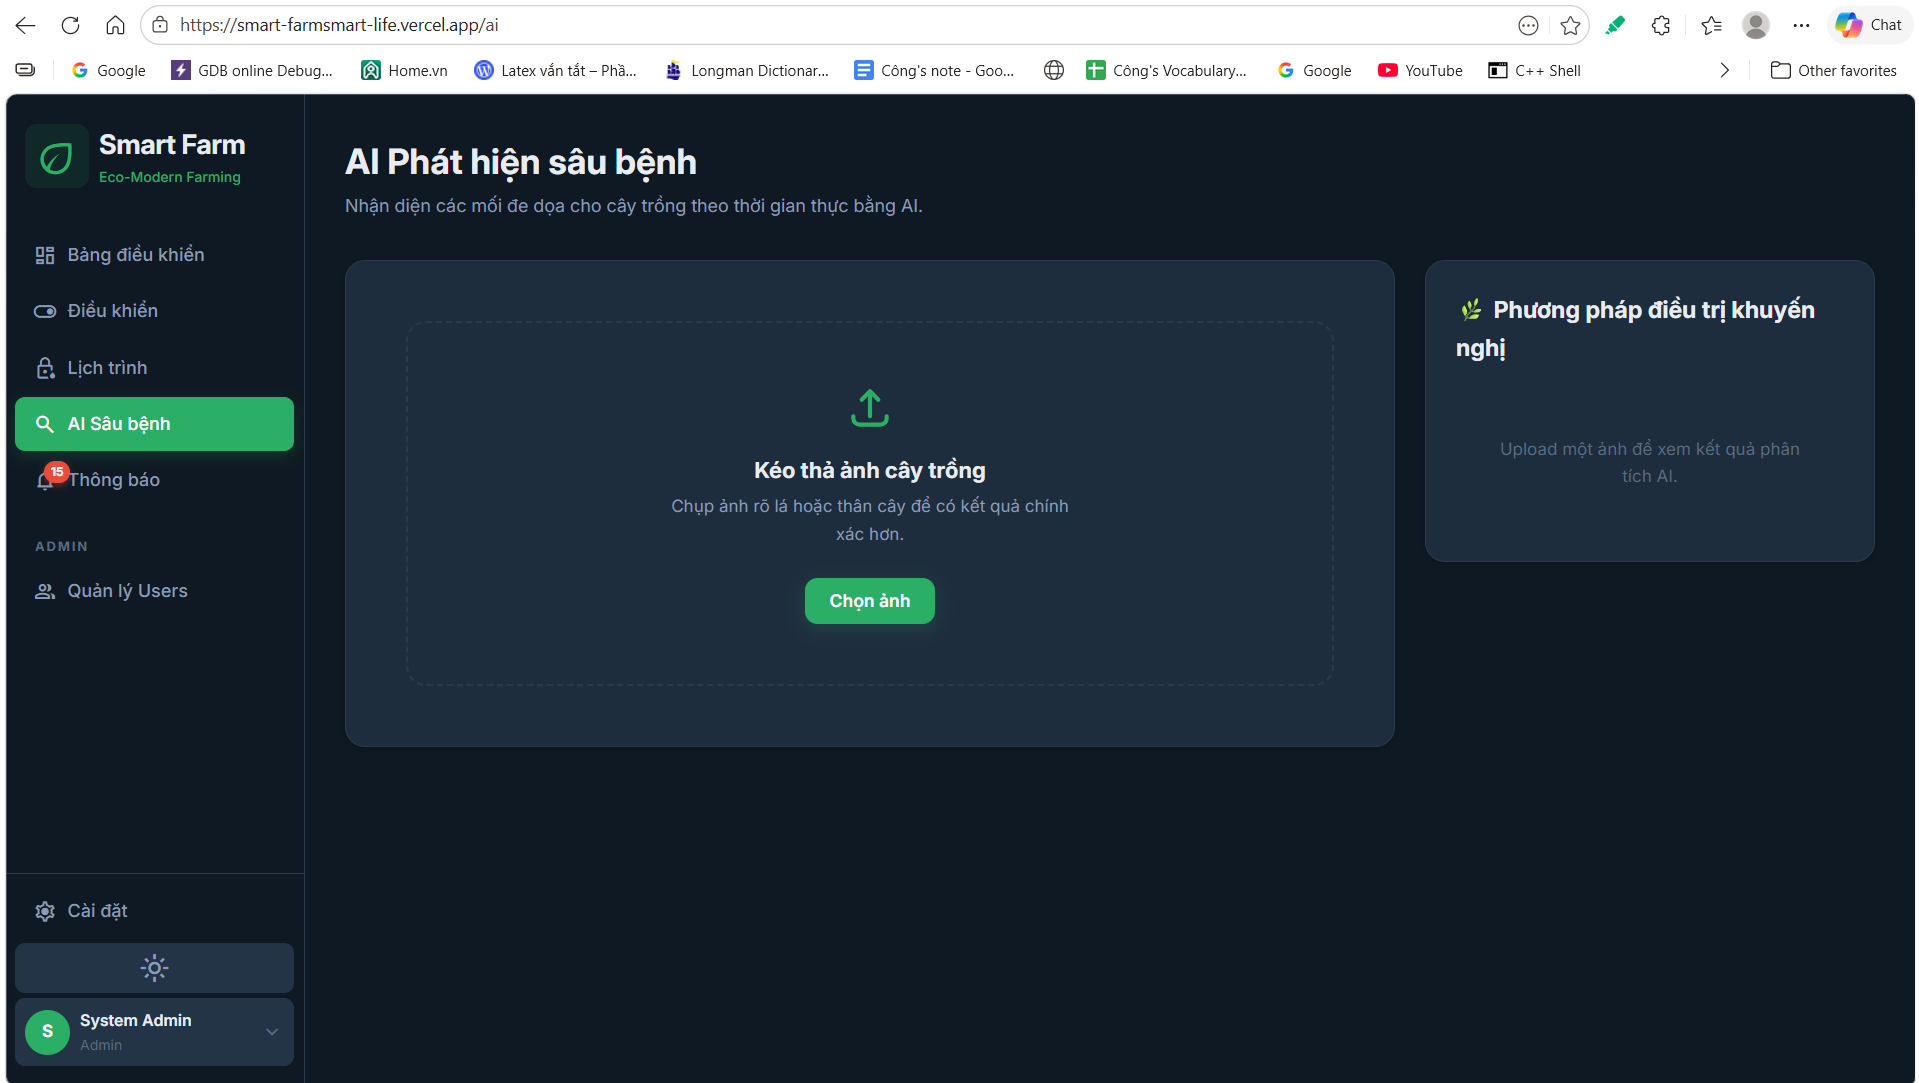
\includegraphics[width=0.9\linewidth]{./Pictures/Task_5/AI_general.png}
	\caption{Giao diện sử dụng AI chẩn đoán bệnh nông nghiệp}
\end{figure}

\indent Mô hình AI hiện tại được hệ thống chia thành 6 lớp phân loại tình trạng của rau màu (cà chua): bao gồm 1 lớp khỏe mạnh và 5 lớp tổn thương khác.
\vspace{0.2cm}
\begin{enumerate}[label=\textbf{\arabic*.}, leftmargin=1.5cm ]
	\item \textbf{Lá cà chua khỏe mạnh}
	\begin{figure}[H]
		\centering
		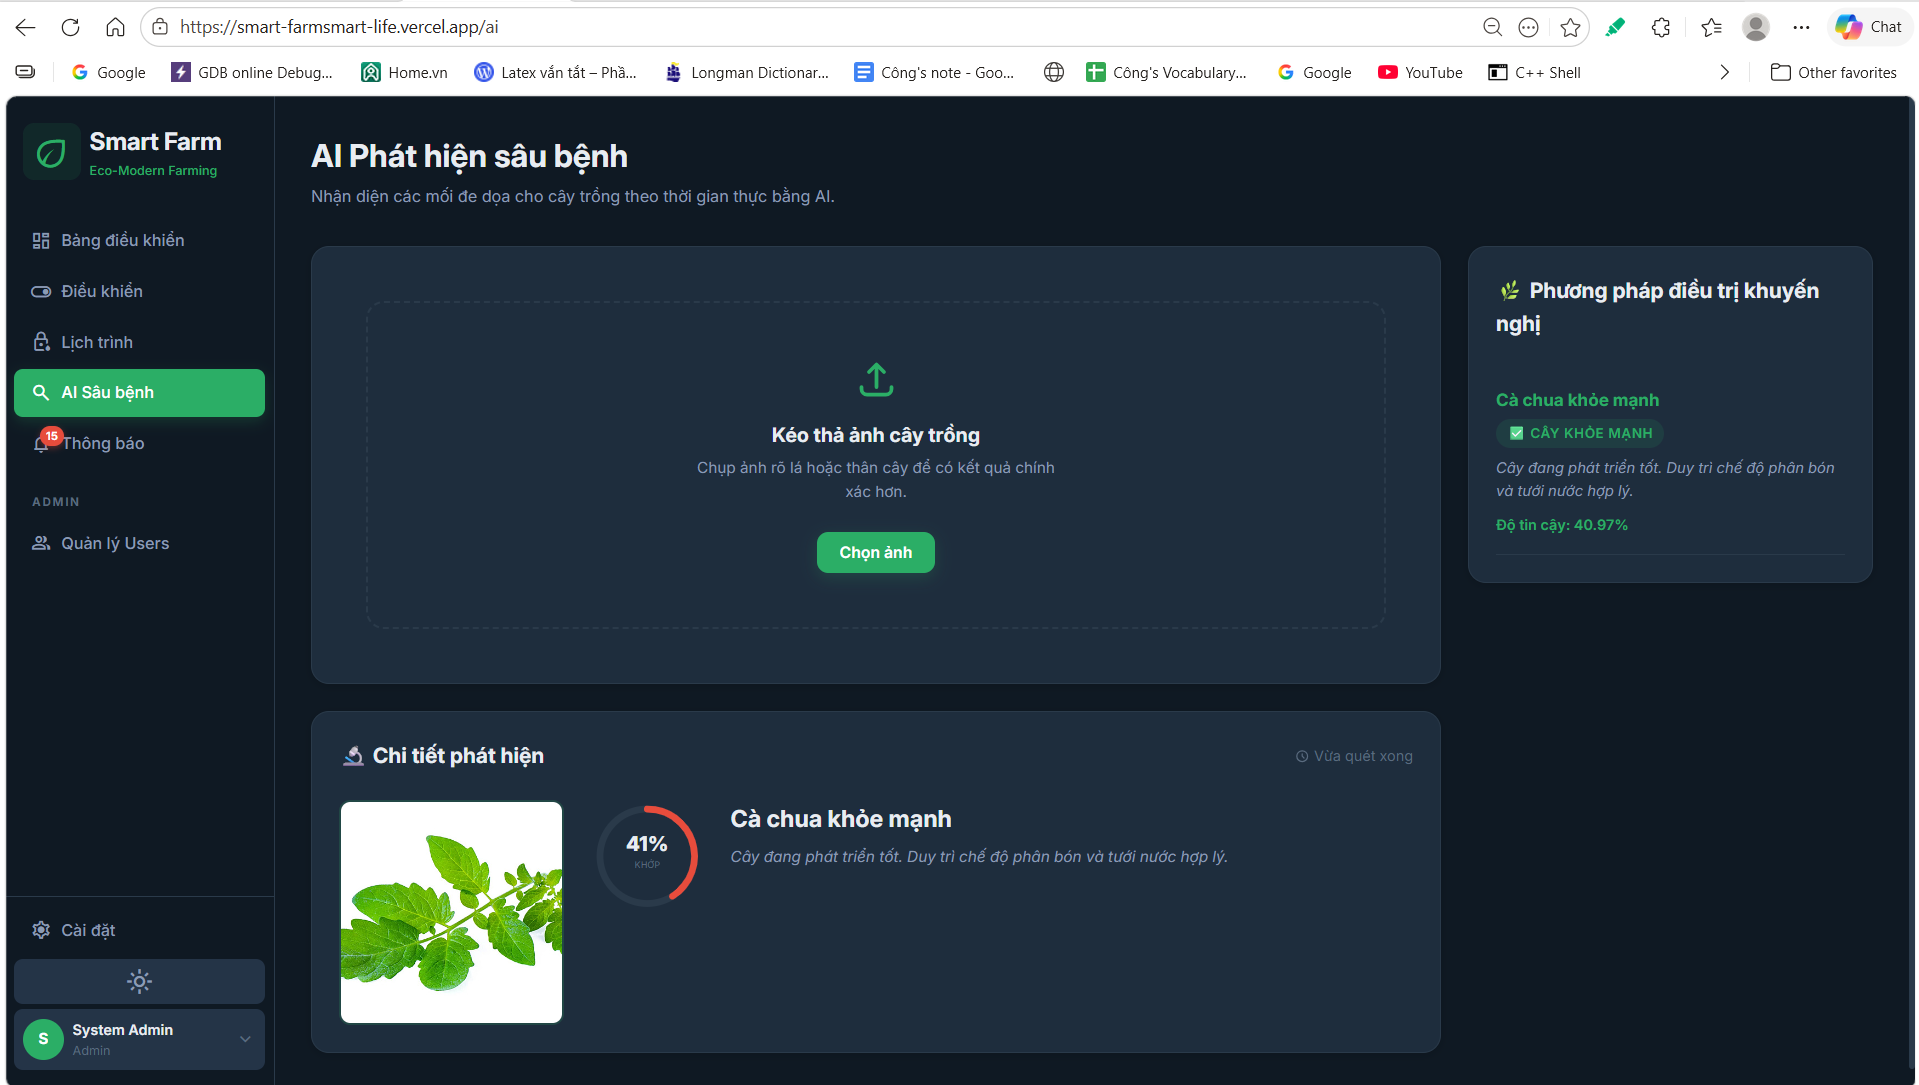
\includegraphics[width=0.8\linewidth]{./Pictures/Task_5/AI_Tomato_Healthy.png}
		\caption{Lá cà chua khoẻ mạnh (Healthy)}
	\end{figure}
	\item \textbf{Lá cà chua bị nhiễm bệnh}
	\begin{figure}[H]
		\centering
		\begin{minipage}{0.5\textwidth}
			\centering
			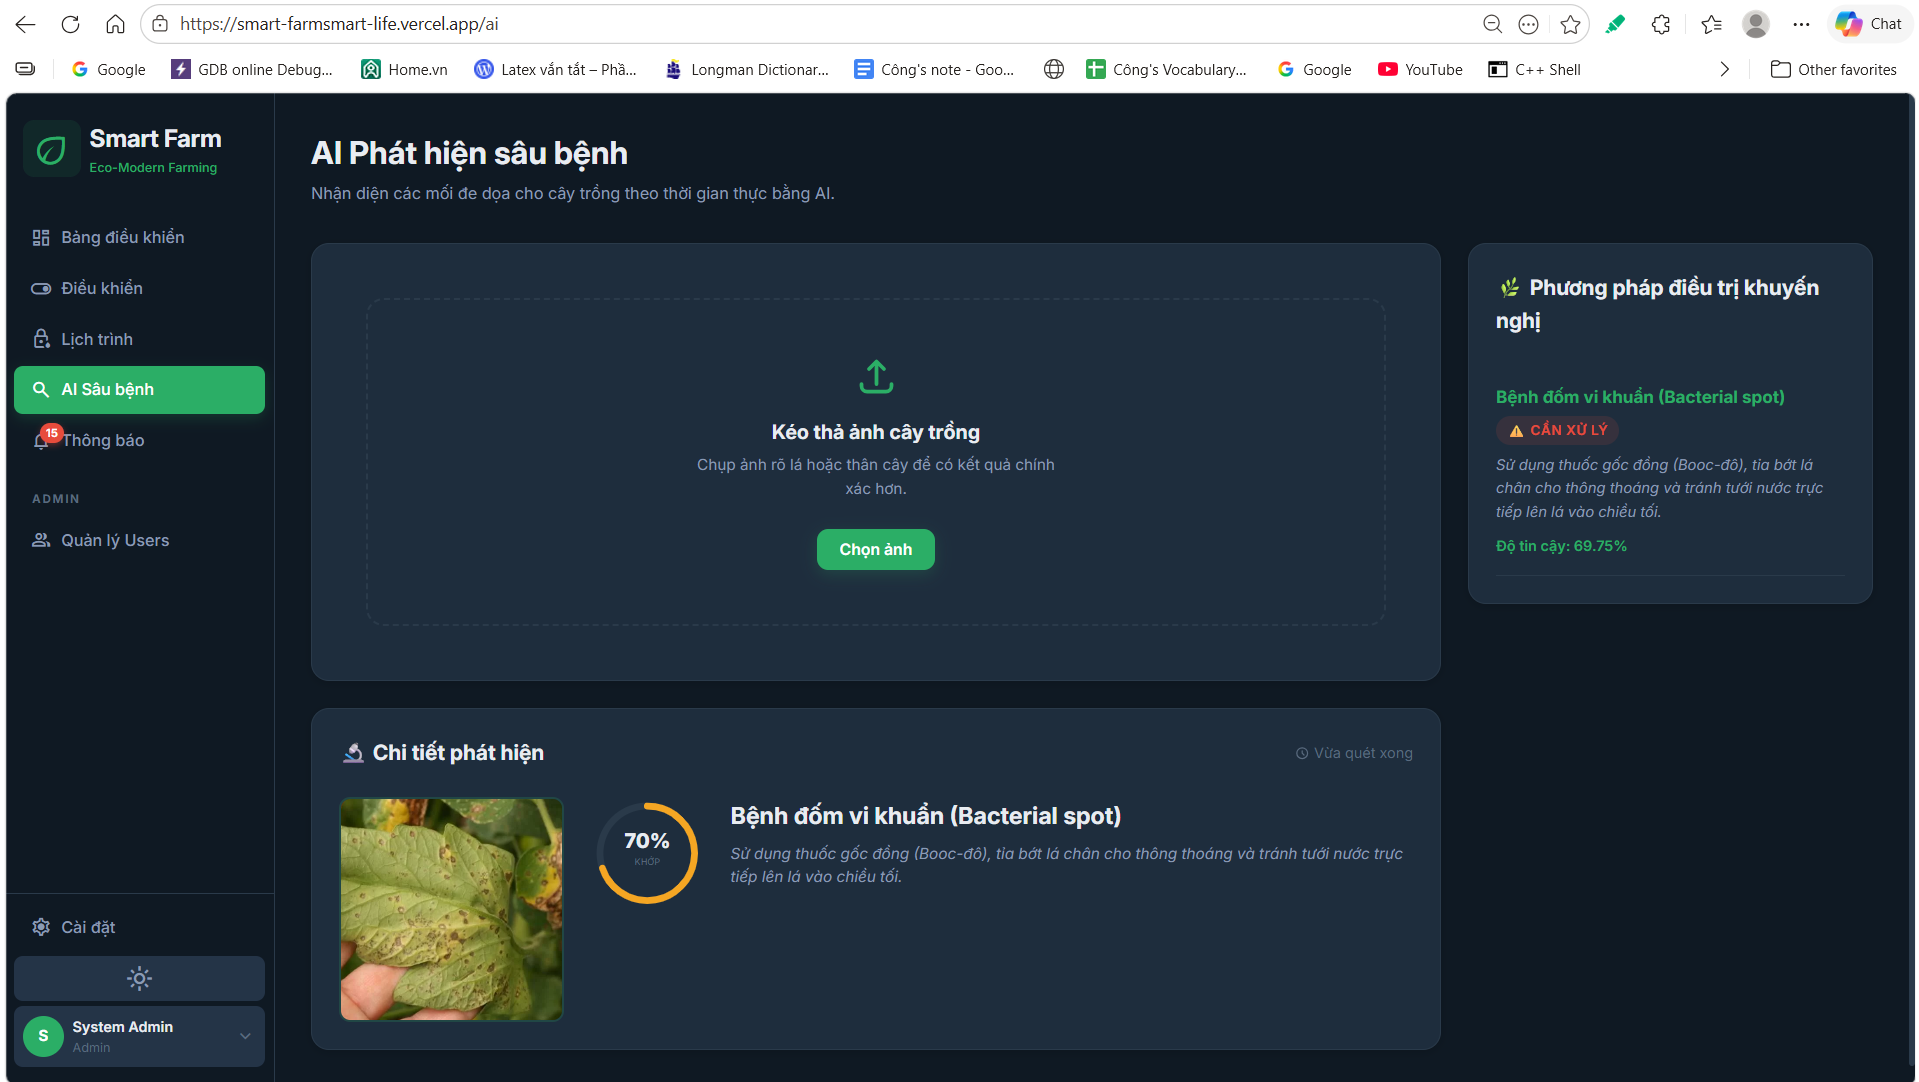
\includegraphics[width=0.95\linewidth]{./Pictures/Task_5/AI_Tomato_Bacterial_Spot.png}\\[0.1cm]
			\textit{Bệnh đốm vi khuẩn\\(Bacterial spot)}
		\end{minipage}\hfill
		\begin{minipage}{0.5\textwidth}
			\centering
			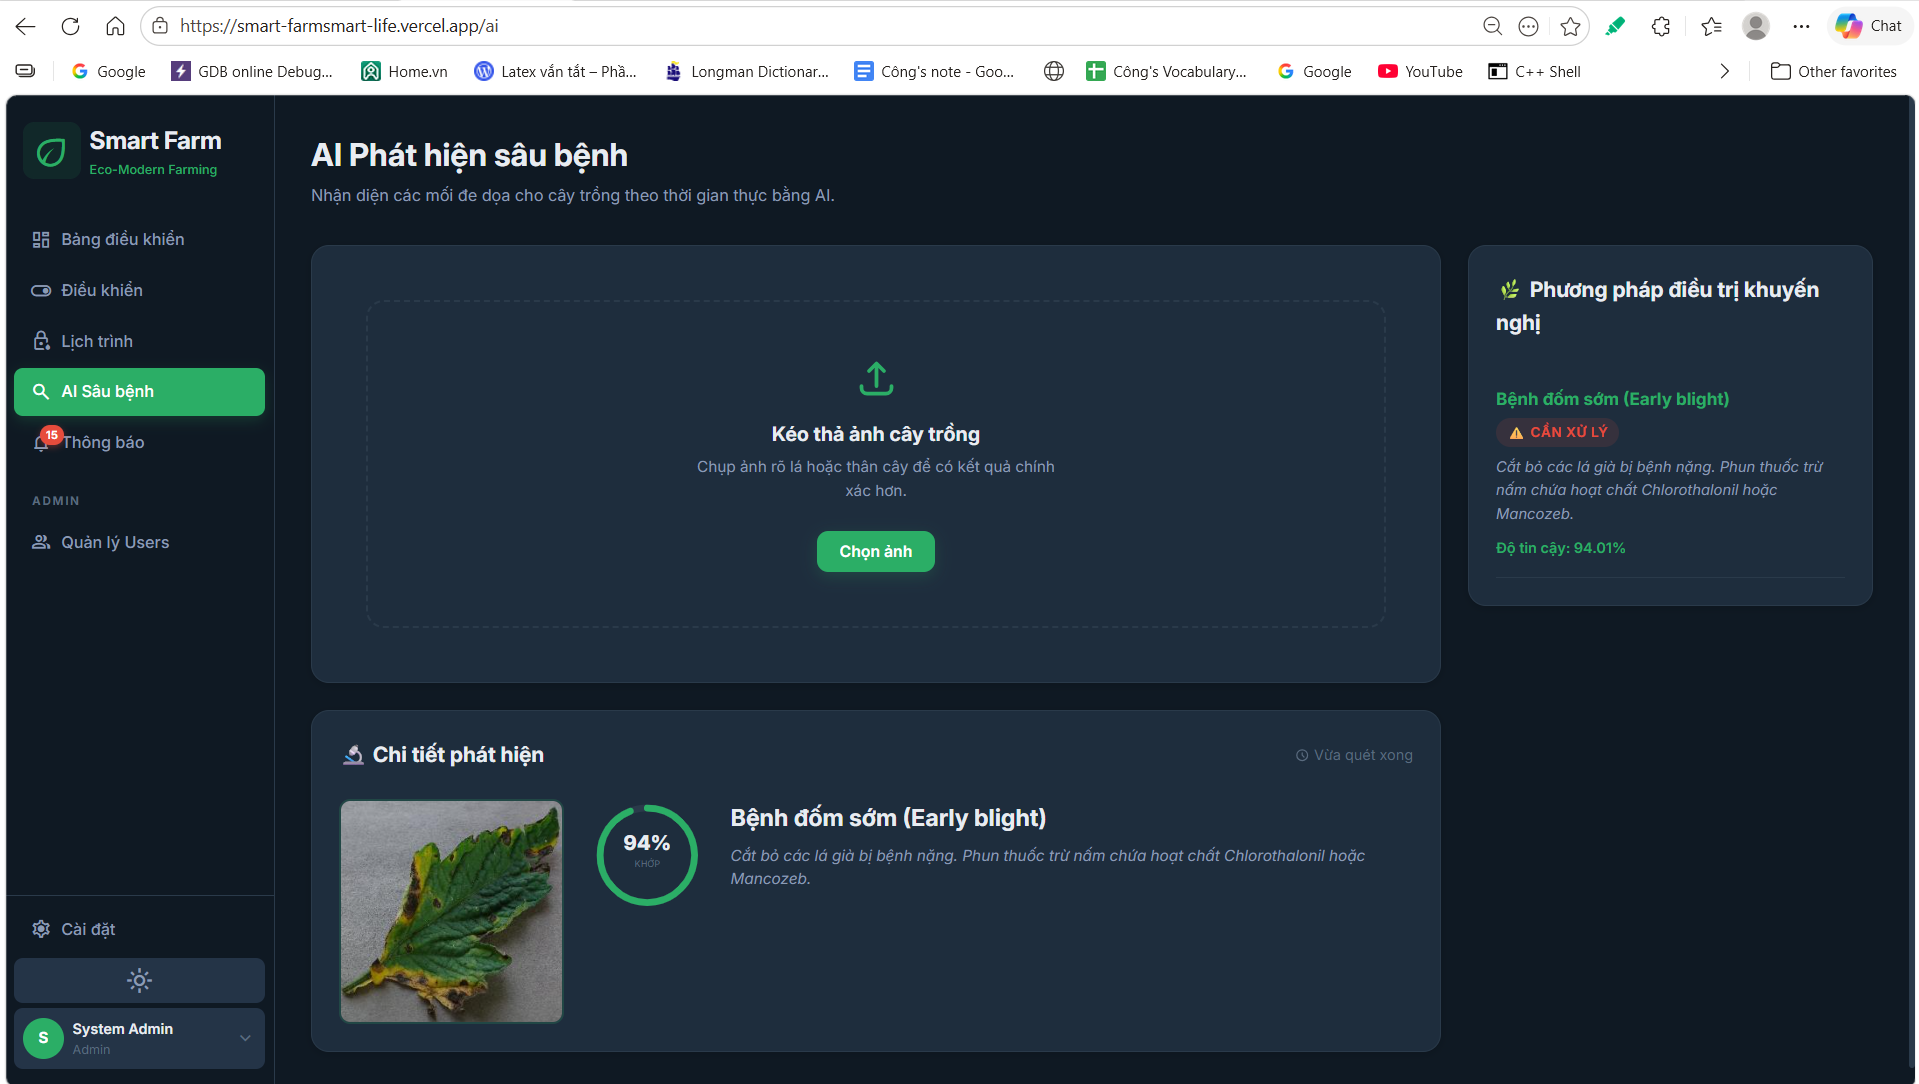
\includegraphics[width=0.95\linewidth]{./Pictures/Task_5/AI_Tomato_Early_Blight.png}\\[0.1cm]
			\textit{Bệnh đốm sớm\\(Early blight)}
		\end{minipage}
		
		\vspace{0.4cm}
		
		\begin{minipage}{0.5\textwidth}
			\centering
			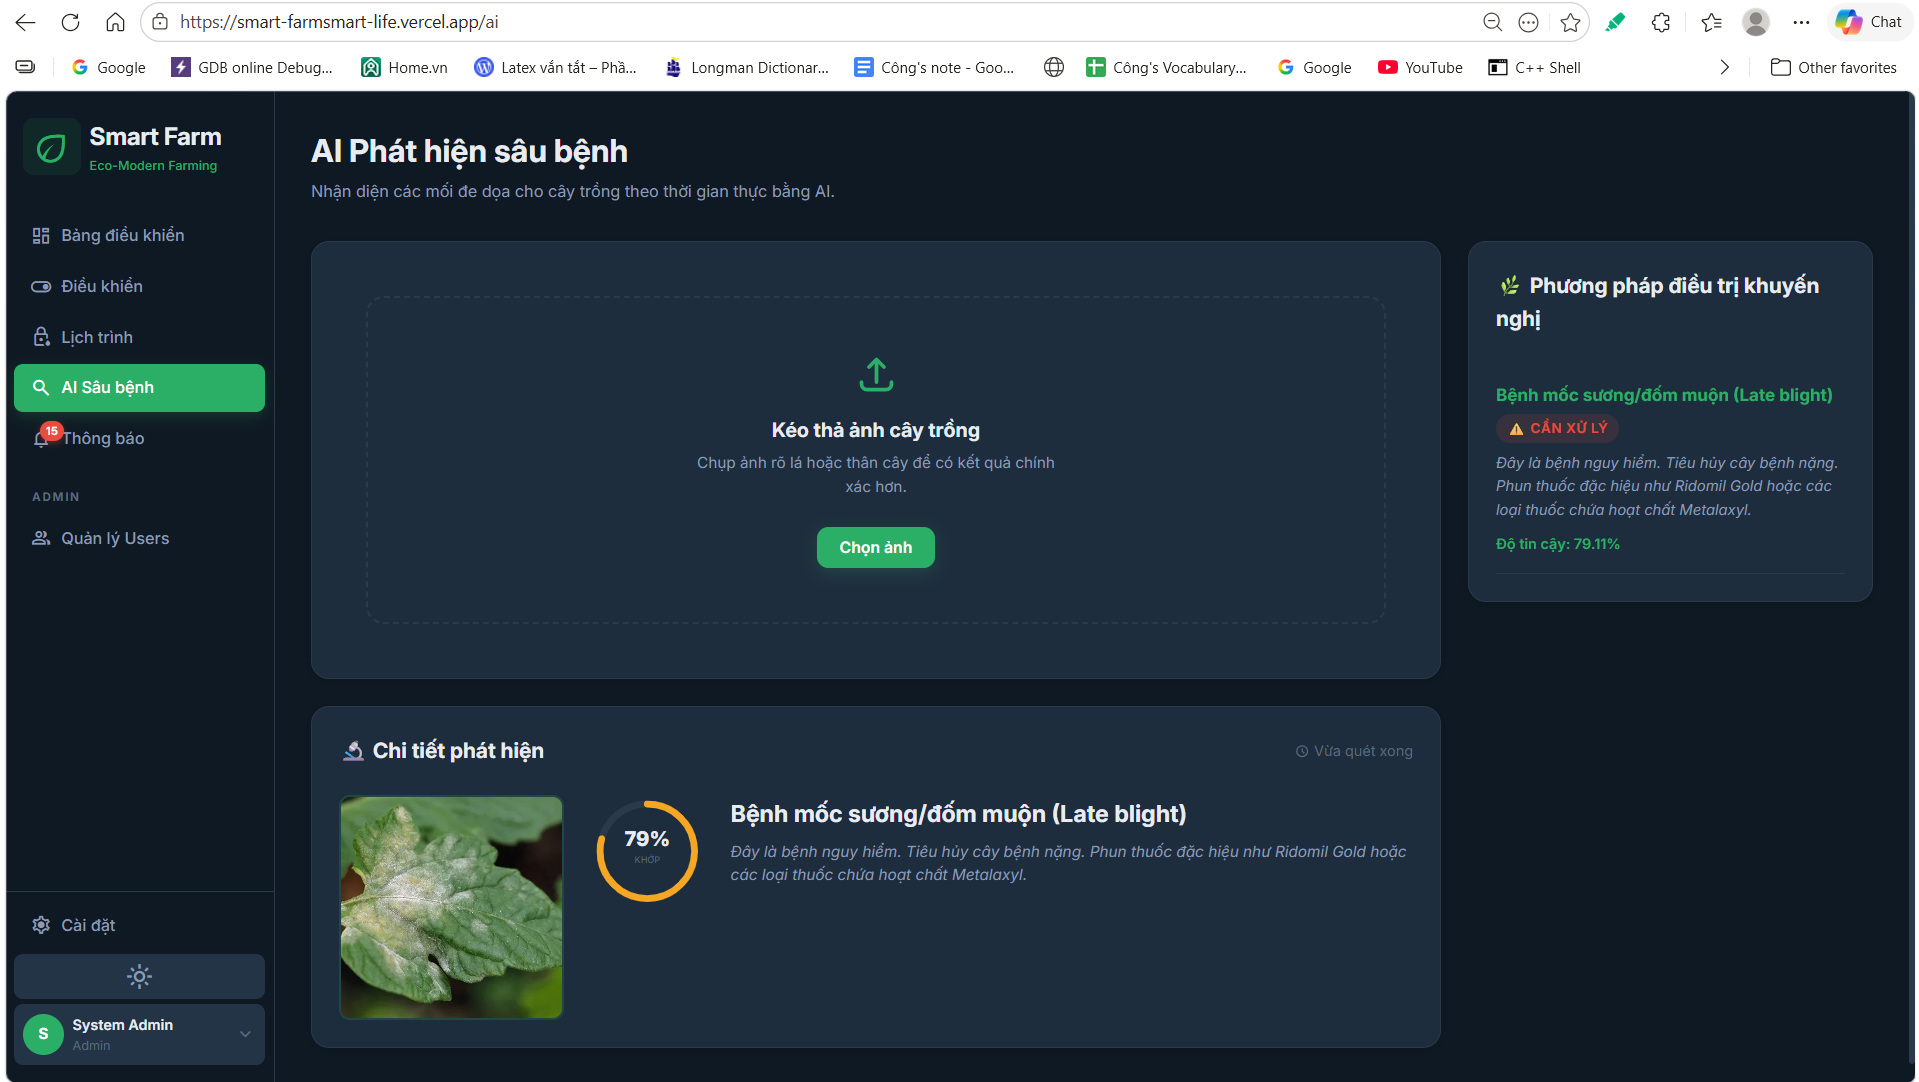
\includegraphics[width=0.95\linewidth]{./Pictures/Task_5/AI_Tomato_Late_Blight.png}\\[0.1cm]
			\textit{Bệnh mốc sương\\(Late blight)}
		\end{minipage}\hfill
		\begin{minipage}{0.5\textwidth}
			\centering
			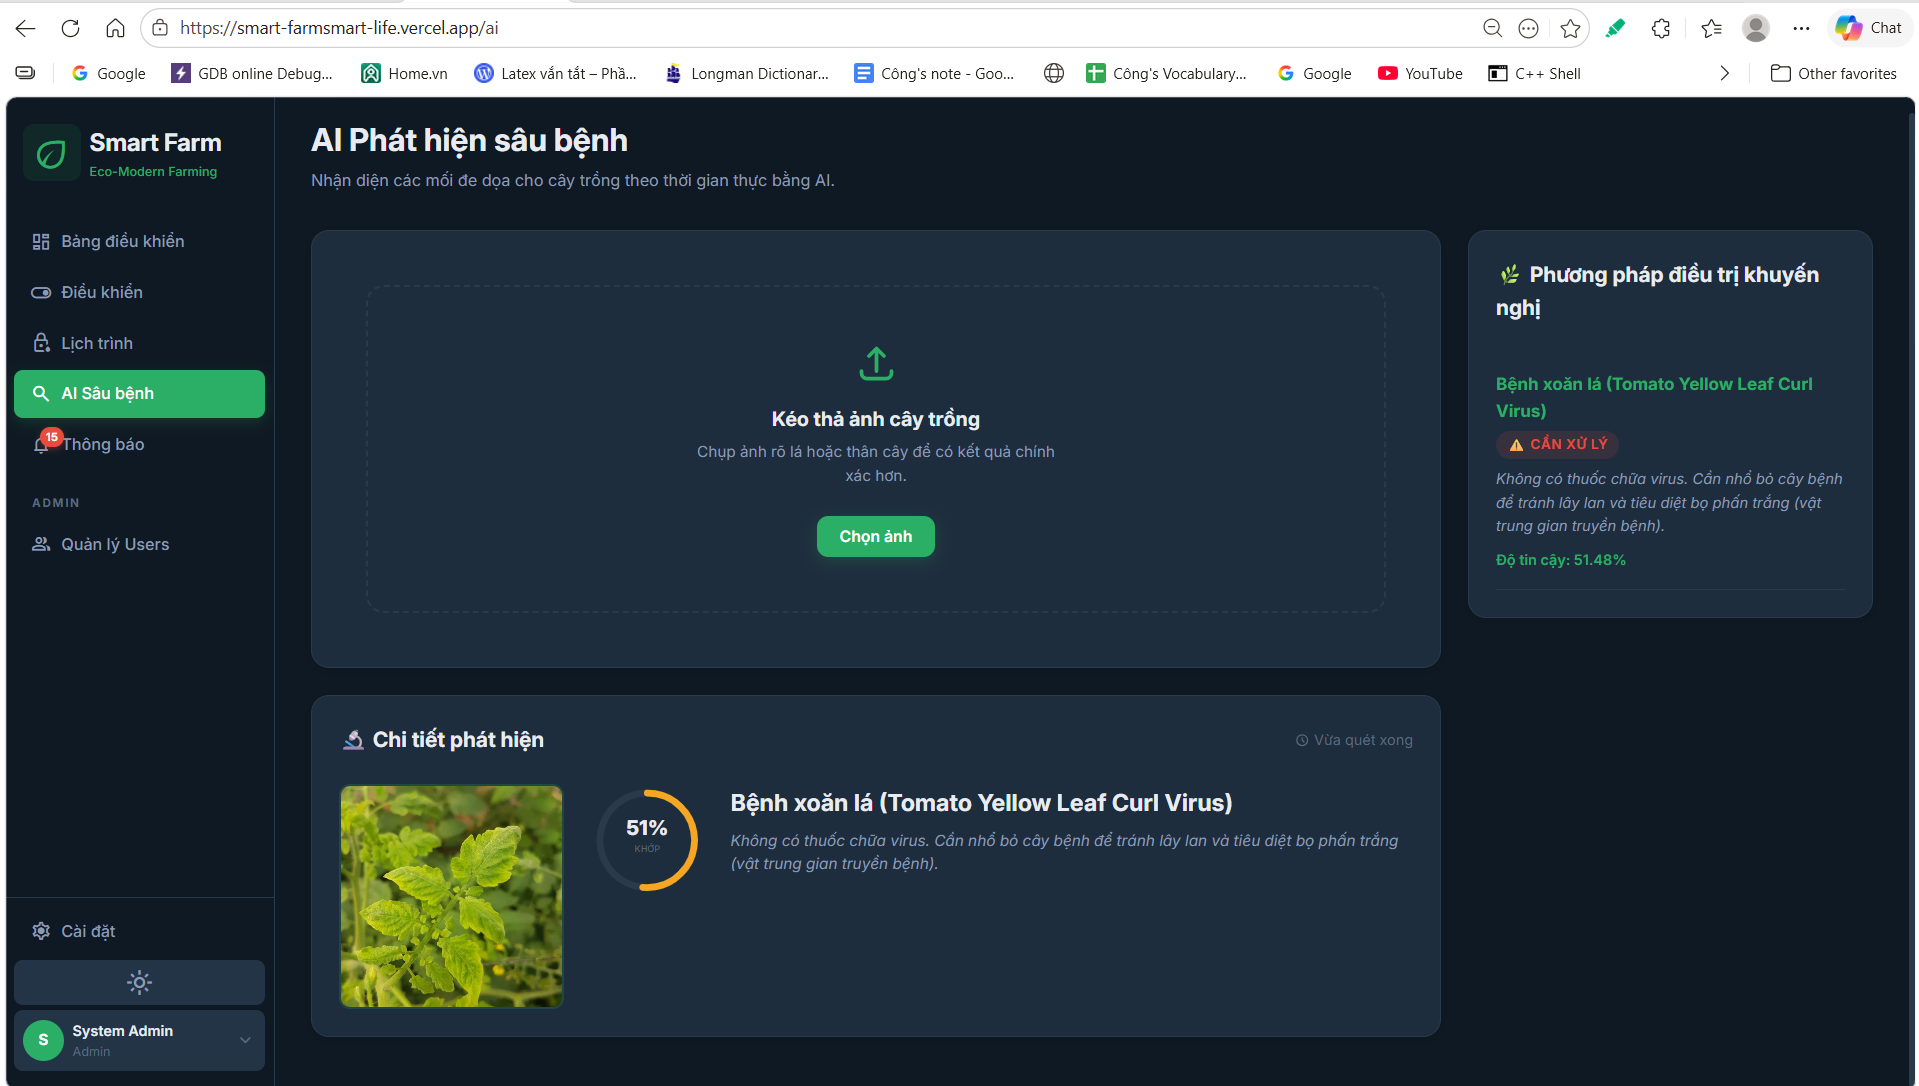
\includegraphics[width=0.95\linewidth]{./Pictures/Task_5/AI_Tomato_Yellow_Leaf_Curl_Virus.png}\\[0.1cm]
			\textit{Bệnh xoăn lá\\(Yellow Leaf Curl)}
		\end{minipage}\hfill
		\begin{minipage}{0.5\textwidth}
			\centering
			\textbf{Cùng một số bệnh lý khác được tích hợp trong mô hình (Leaf Mold,...)}
		\end{minipage}
		\caption{Các tập mẫu kết quả nhận diện trên mô hình thực tế}
	\end{figure}
\end{enumerate}
%TODO: Thêm phần mô tả về cách thức hoạt động của AI dựa trên phần xử lý hình ảnh thuộc yolofarm\server\api\main.py

	\section{Mô tả design pattern và Deploy hệ thống}
\subsection{Kiến trúc các design pattern được sử dụng}
\indent Sau quá trình nghiên cứu và phát triển phần mềm cho hệ thống YoloFarm, nhóm đã áp dụng các Design Pattern (mẫu thiết kế) sau đây để đảm bảo kiến trúc rõ ràng, dễ bảo trì và dễ mở rộng:
\setlist[enumerate]{leftmargin=*,topsep=0pt,itemsep=2pt,parsep=0pt}
\setlist[itemize]{leftmargin=*,topsep=0pt,itemsep=2pt,parsep=0pt}
\begin{longtable}{|P{4.8cm}|m{10cm}|}\hline
    \hline
    \textbf{Design Pattern} & \centering\arraybackslash\textbf{Chi tiết áp dụng trong dự án} \\
    \hline

    \textbf{MVC (Model - View - Controller)} & Thư mục \texttt{server/src/models/} chứa các class/đối tượng định nghĩa cách tương tác với bảng trong cơ sở dữ liệu MySQL (Model). Thư mục \texttt{server/src/controllers/} chịu trách nhiệm nhận request từ người dùng, gọi các logic để xử lý dữ liệu và trả về kết quả (Controller). Phía Frontend ứng dụng React trong thư mục \texttt{client/src/pages/} và \texttt{components/} hiển thị dữ liệu lên màn hình (View). \\
    \hline
    \textbf{Middleware Pattern} & Áp dụng trong xây dựng API của Express.js nằm tại thư mục \texttt{server/src/middleware/}. Các request từ Client trước khi chuyển đến Controller sẽ đi qua các Middleware chặn lại để thực hiện: xác thực người dùng (Authentication qua JWT), kiểm tra tính hợp lệ dữ liệu và phân quyền hệ thống (Authorization). \\
    \hline
    \textbf{Observer / Pub-Sub Pattern} & Nhằm thiết lập truyền tải nhận dữ liệu thời gian thực. Bằng cách sử dụng giao thức MQTT kết nối với máy chủ Adafruit IO, server đóng vai trò chuyển tiếp như một "Publisher" và "Subscriber" lắng nghe dữ liệu liên tục do phần cứng gửi tới. Ngoài ra, Socket.IO cũng sử dụng Pub-Sub để đẩy tự động (push) các cảnh báo thông báo trực tiếp lên giao diện Frontend. \\
    \hline
    \textbf{Singleton Pattern} & Đảm bảo chỉ khởi tạo một thể hiện (instance) duy nhất của đối tượng trong toàn hệ thống. Ví dụ: instance kết nối cơ sở dữ liệu ở \texttt{server/src/config/db.js} hoặc module MQTT Node-Client luôn chỉ tồn tại một bản sao xuyên suốt ứng dụng. Với React Frontend, sử dụng React Context (như \texttt{AuthContext}, \texttt{ThemeContext}) qua Provider cũng là ứng dụng tương đương của Singleton để cung cấp trạng thái toàn cục (global state) cho ứng dụng. \\\hline
\end{longtable}
\subsection{Deploy hệ thống}
\indent Việc triển khai của YoloFarm được tổ chức theo đúng cấu trúc repo hiện tại: phần giao diện nằm ở \texttt{client/}, backend Node.js nằm ở \texttt{server/}, còn dịch vụ AI chạy tách biệt như một FastAPI space/container riêng. Trong giai đoạn phát triển, nhóm ưu tiên chạy local bằng \texttt{pnpm dev} để đồng bộ frontend, backend và AI service; khi đưa lên môi trường triển khai, các thành phần được đóng gói theo Docker Compose hoặc các nền tảng hosting tương ứng để giữ cấu hình nhất quán giữa máy lập trình và môi trường chạy thực tế.

\begin{figure}[H]
	\centering
	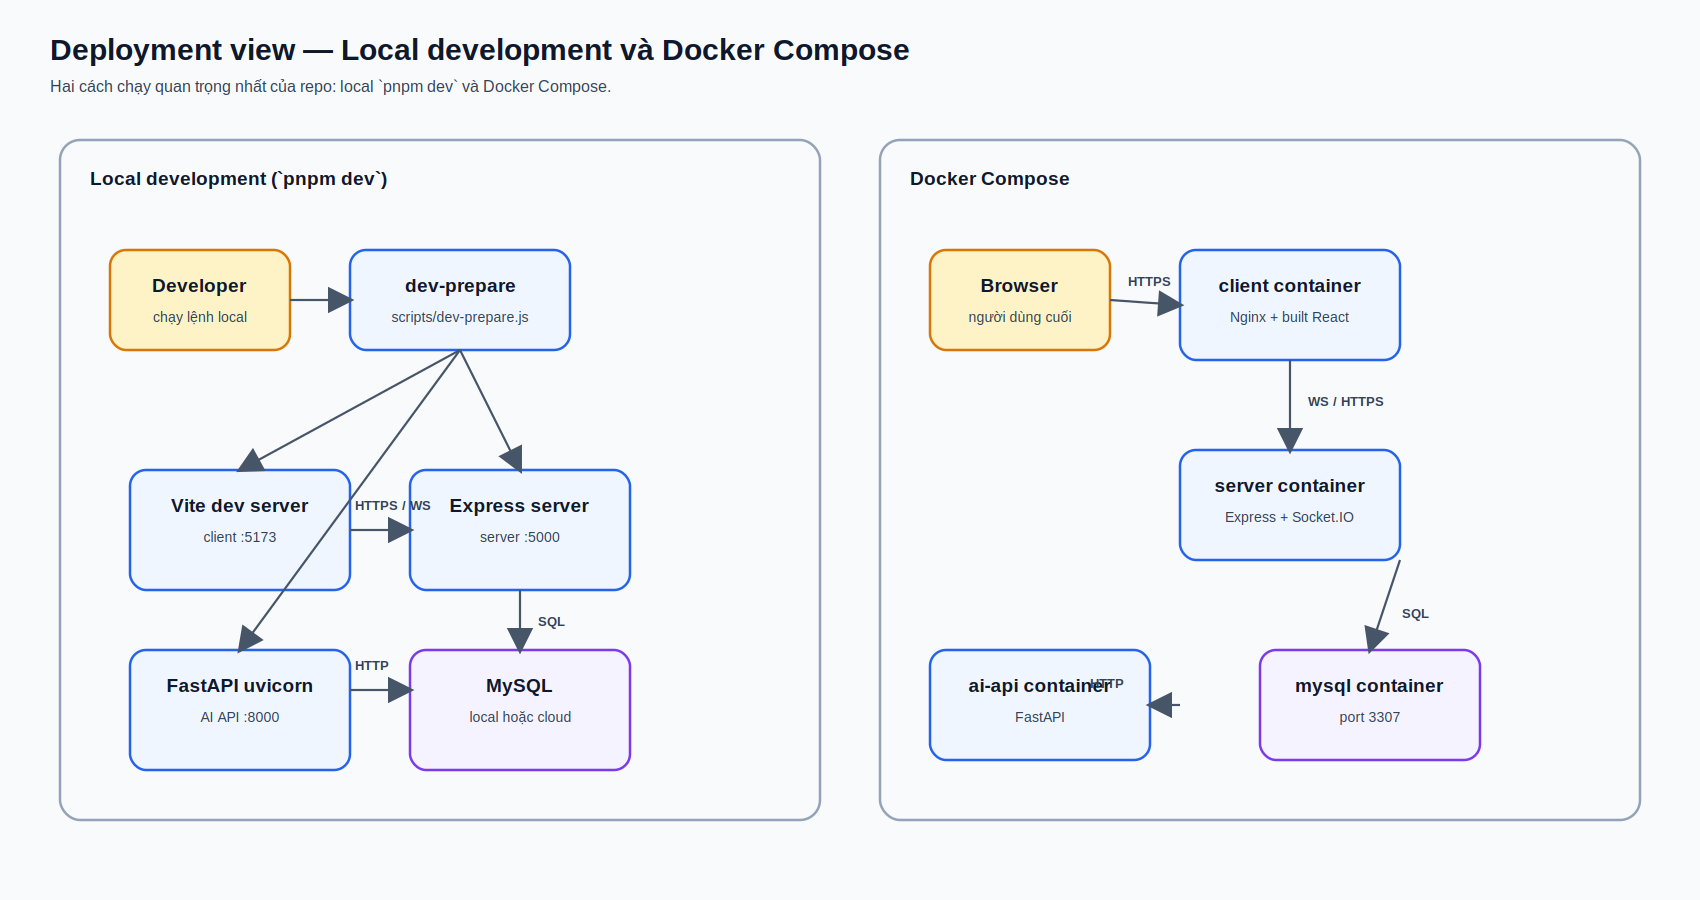
\includegraphics[width=0.92\linewidth]{./Pictures/Task_6/architecture/deployment-view.png}
	\caption{Sơ đồ triển khai của YoloFarm theo hai chế độ chạy local và Docker Compose}
\end{figure}

\subsubsection{Deploy frontend}
\indent Giao diện frontend của YoloFarm được triển khai trên \textbf{Vercel}. Mã nguồn được quản lý tại kho GitHub \texttt{yolofarm---group-6---L05---HK252}, từ đó Vercel tự động đồng bộ và kích hoạt quy trình CI/CD cho nhánh triển khai.

\indent Trên Vercel, các biến môi trường (Environment Variables) được cấu hình để frontend gọi đúng backend đang chạy trên Hugging Face Spaces, cụ thể là biến \texttt{VITE\_API\_URL} trỏ đến \url{https://cong2005-smartfarm-ai.hf.space/api}. Nhờ đó, người dùng có thể truy cập giao diện YoloFarm qua đường dẫn công khai: \url{https://smart-farmsmart-life.vercel.app/}.

\begin{figure}[H]
	\centering
	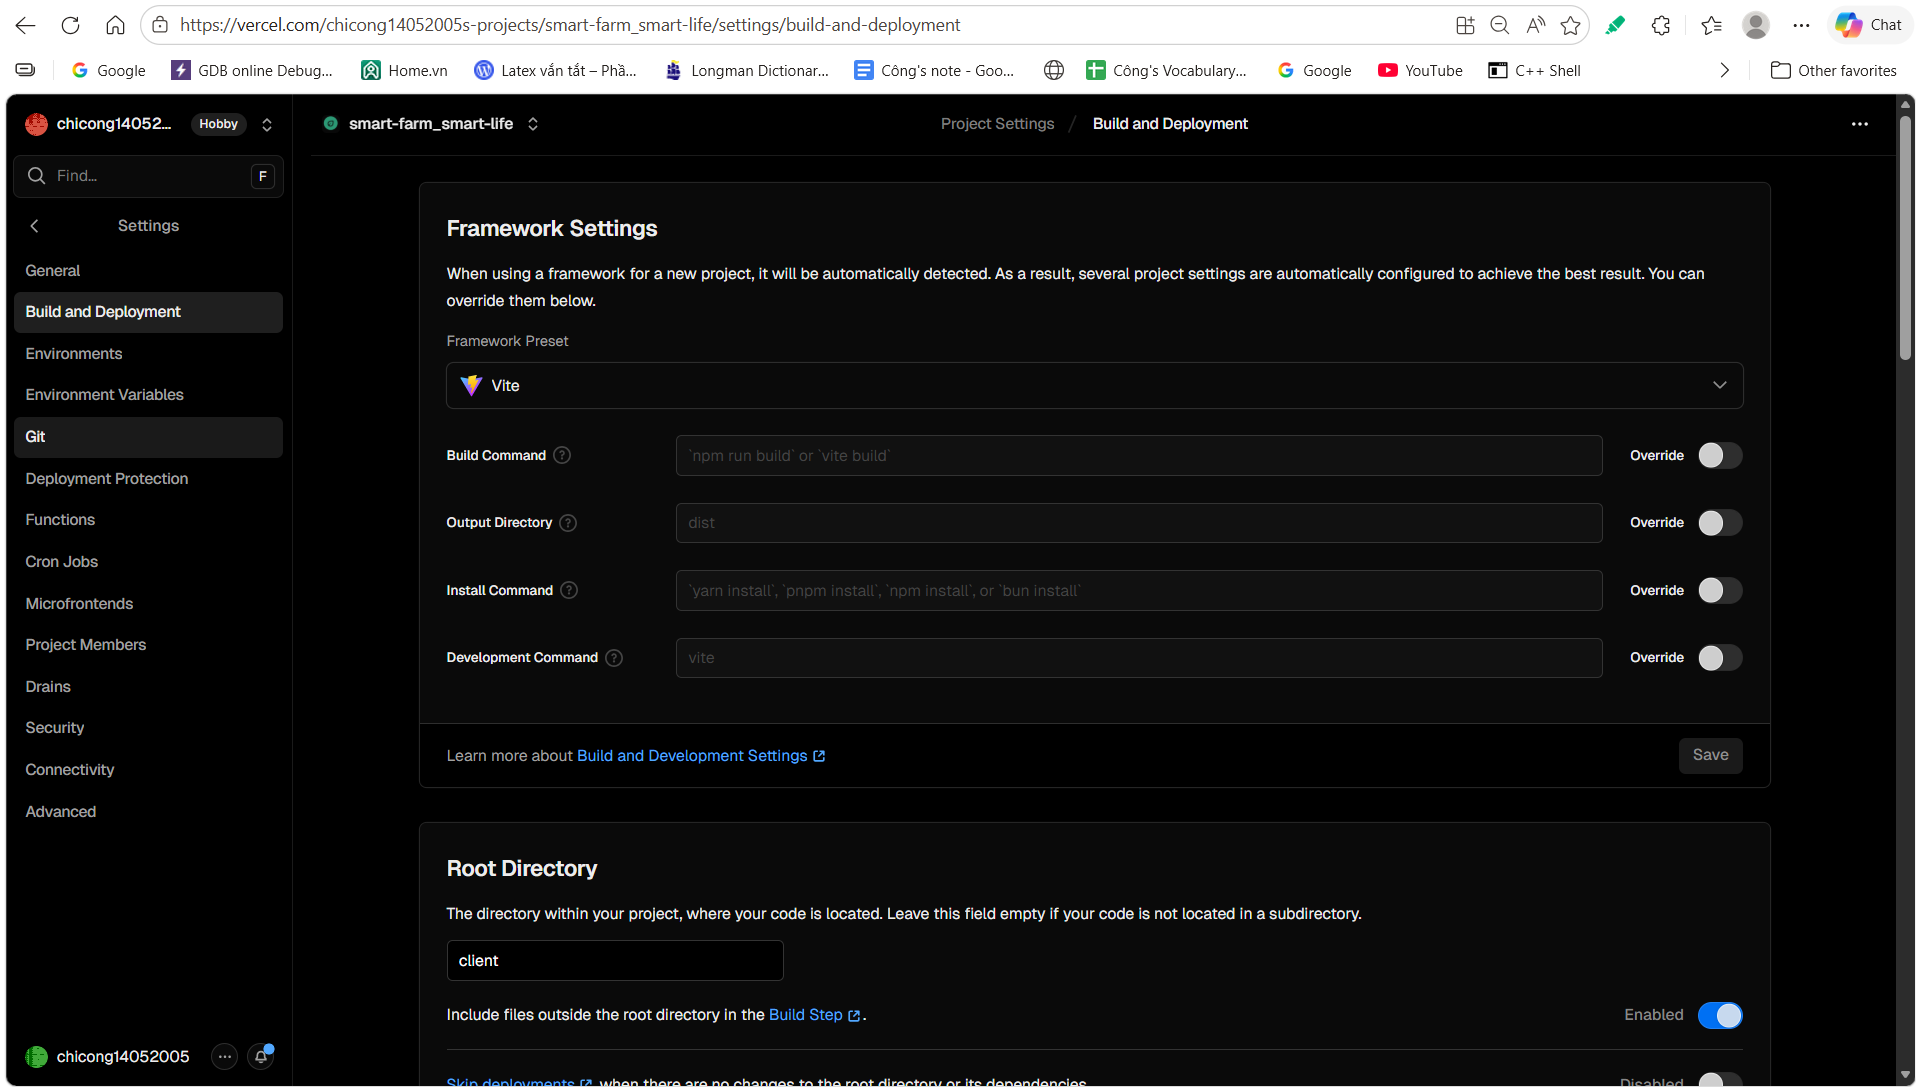
\includegraphics[width=0.8\linewidth]{./Pictures/Task_6/frontend_vercel.png}
	\caption{Giao diện Deployment phần mã nguồn Frontend trên Vercel}
\end{figure}
\subsubsection{Deploy backend}
\subsubsubsection{Phần server}
\indent Backend server của YoloFarm được triển khai trên \textbf{Hugging Face Spaces}. Thành phần Node.js được đóng gói bằng \texttt{Dockerfile} để giữ nguyên hành vi giữa môi trường local và môi trường chạy thật, đồng thời tách biệt rõ phần server với phần giao diện. Các lệnh khởi động và biến môi trường được khai báo ngay trong cấu hình container, giúp server có thể kết nối ổn định tới dịch vụ AI thông qua biến \texttt{AI\_API\_URL}.

\begin{figure}[H]
	\centering
	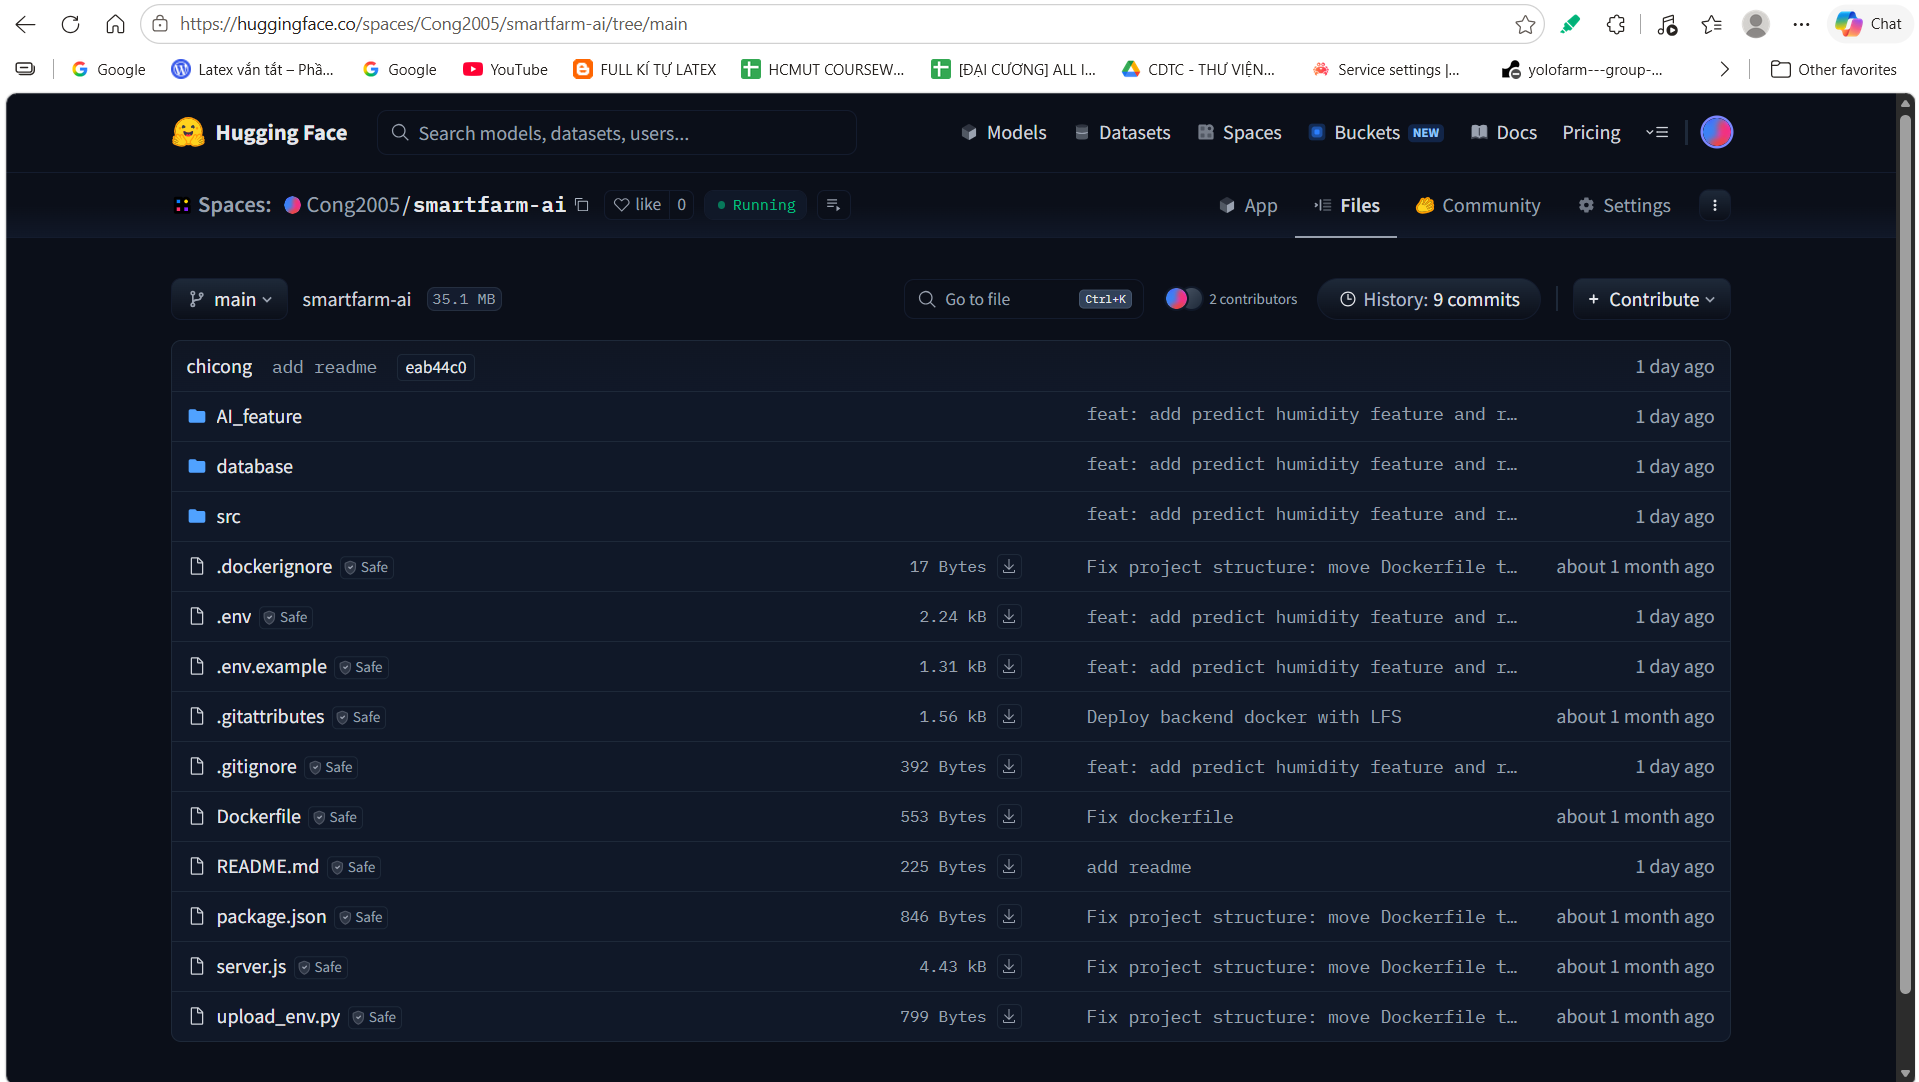
\includegraphics[width=0.8\linewidth]{./Pictures/Task_6/backend_server_files.png}
	\caption{Danh sách mã nguồn Backend Server chạy trên Hugging Face Spaces}
\end{figure}

\subsubsubsection{Phần các tính năng AI}
\indent Dịch vụ AI của YoloFarm được vận hành như một \textit{Space độc lập} để tối ưu tài nguyên cho suy luận mô hình. Space này tự cài các thư viện Python được khai báo trong \texttt{requirements.txt} và sử dụng mô hình đã huấn luyện tại tệp \url{https://huggingface.co/spaces/Cong2005/SmartFarm_api/blob/main/pest_detection/api/plant_disease_recog_model_pwp_5.keras} để phân loại bệnh lá cây từ ảnh đầu vào.

\begin{figure}[H]
	\centering
	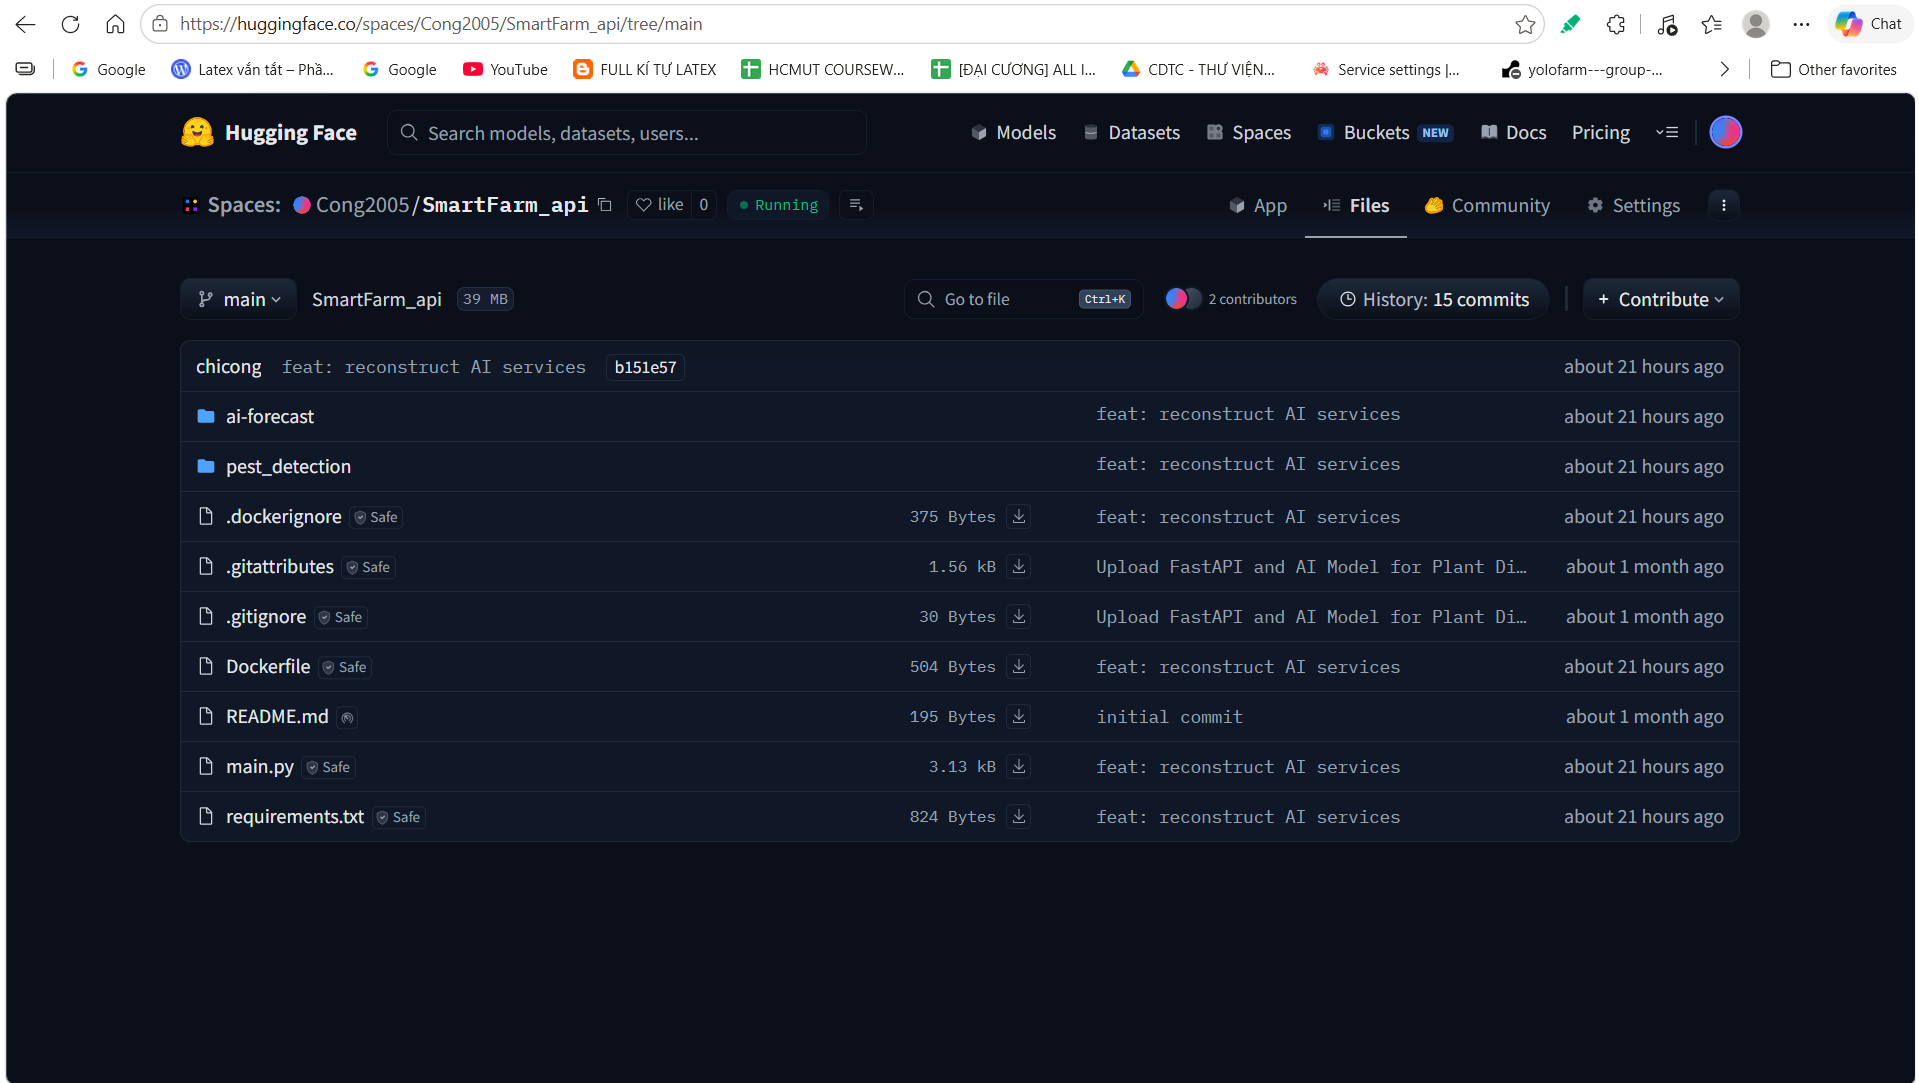
\includegraphics[width=0.8\linewidth]{./Pictures/Task_6/backend_AI_files.png}
	\caption{Hệ thống tự động biên dịch và chạy các mô hình AI}
\end{figure}
\subsubsection{Cơ chế hoạt động}
\indent Toàn thể kiến trúc YoloFarm được thiết kế theo hướng dễ mở rộng và tách biệt trách nhiệm:
\begin{itemize}
    \item \textbf{Luồng tương tác chính:} Người dùng làm việc trên frontend, frontend gửi request đến backend Node.js, backend xử lý nghiệp vụ và trả kết quả về giao diện. Cách tách lớp này giúp YoloFarm dễ bảo trì và phù hợp với cả chế độ chạy local lẫn triển khai container.
    \item \textbf{Luồng tải ảnh, chẩn đoán hoặc dự đoán độ ẩm:} Khi người dùng gửi ảnh lá cây để nhận diện bệnh, backend sẽ chuyển ảnh sang dịch vụ AI FastAPI độc lập, nhận kết quả dự đoán dạng JSON rồi phản hồi lại frontend để hiển thị cho người dùng. Mặt khác, khi bấm nút "Cập nhật dự báo" thì hệ thống dựa vào kho dữ liệu lưu trữ độ ẩm thực tế của ít nhất 24 giờ trước thời điểm cập nhật dự báo và dự đoán độ ẩm cho 24 giờ kế tiếp. Sau đó, kết quả dự đoán được trả về giao diện.
\end{itemize}
	\section{Đường link hệ thống và mã nguồn}
\begin{enumerate}[label=\textbf{\arabic*.}]
	\item \textbf{Đường link hệ thống:} \href{https://smart-farmsmart-life.vercel.app/}{\textbf{\textcolor{red}{Tại đây!}}}
	\item \textbf{Đường link mã nguồn Github:} \href{https://github.com/chicong14052005/yolofarm---group-6---L05---HK252}{\textbf{\textcolor{blue}{Tại đây!}}}
\end{enumerate}
\end{document}
%
    \endinput
  }%
\else
  \let\prismpreambleaction\relax
\fi
\prismpreambleaction
\RequirePackage{fix-cm}
\documentclass[a4paper]{article}
%\usepackage{vntex}
\usepackage[utf8]{inputenc}
\usepackage[T5]{fontenc}
\usepackage[dvipsnames]{xcolor}
\usepackage{a4wide,amssymb,epsfig,latexsym,multicol,array,hhline,fancyhdr}
%\usepackage[english,vietnam]{babel}
%\usepackage[utf8]{inputenc}
%\usepackage[colorlinks=true, linkcolor=red, urlcolor=red]{hyperref}
%\usepackage{hyperref}
%\usepackage[utf8]{inputenc}
%\usepackage[francais]{babel}
\usepackage[normalem]{ulem}
\usepackage{lipsum}
%\usepackage{soul}
\usepackage{caption}
\usepackage{float}
\renewcommand{\figurename}{}
\usepackage{wasysym}
\usepackage{enumerate}
\usepackage{enumitem}
\usepackage[makeroom]{cancel}

%\let\Vint\relax  % Xóa lệnh \Vint cũ (nếu có)
\let\iint\relax
\let\iiint\relax
\usepackage{amsmath}

\usepackage{amsfonts}
\usepackage{amssymb}
\usepackage{amsthm}
\usepackage{multicol,longtable,amscd}
\usepackage{diagbox}%Make diagonal lines in tables
\usepackage{booktabs}
\usepackage{alltt}
\usepackage[framemethod=tikz]{mdframed}% For highlighting paragraph backgrounds
\usepackage{caption,subcaption}
\usepackage{listings}
\usepackage{color}
\usepackage{lastpage}
\usepackage[lined,boxed,commentsnumbered]{algorithm2e}
\usepackage{color}
\usepackage{graphicx}							% Standard graphics package
\graphicspath{{./}{../}}
\usepackage{array}
\usepackage{tabularx, caption}
\usepackage{multirow}
\usepackage{multicol}
\usepackage{rotating}
\usepackage{graphics}
\usepackage{geometry}
\usepackage{setspace}
\usepackage{epsfig}
\usepackage{tikz}
\usepackage{titlesec}
\usepackage{tocloft}
\usetikzlibrary{calc}
\usepackage{eso-pic,xcolor}
%normalsize\usepackage[font=small, labelfont=bf, labelsep=colon]{caption}
\usetikzlibrary{arrows,decorations.pathmorphing,decorations.pathreplacing,decorations.shapes,backgrounds}

%\usepackage{pstcol} % PSTricks with the standard colocaptionr package
\usepackage[normalem]{ulem}
\newtheorem{theorem}{{\bf Định lý}}

\newtheorem{property}{{\bf Tính chất}}
\newtheorem{proposition}{{\bf Mệnh đề}}
\newtheorem{corollary}[proposition]{{\bf Hệ quả}}
\newtheorem{lemma}[proposition]{{\bf Bổ đề}}
\theoremstyle{definition}
\newtheorem{exer}{Bài toán}
\def\thesislayout{	% A4: 210 × 297
	\geometry{
		a4paper,
		total={160mm,240mm},  % fix over page
		left=30mm,
		top=30mm,
	}
}
\thesislayout

\makeatletter
\renewcommand\paragraph{\@startsection{paragraph}{4}{\z@}%
	{3.25ex \@plus1ex \@minus.2ex}%
	{1ex \@plus.2ex}%
	{\normalfont\normalsize\bfseries}}
\makeatother

\renewcommand{\baselinestretch}{1.5} % Giãn dòng 1.5
% \setlength{\parskip}{6pt} % Spacing after
\usepackage{indentfirst}
\setlength{\parindent}{1cm}

%\usepackage{fancyhdr}
\setlength{\headheight}{40pt}
\pagestyle{fancy}
\fancyhead{} % clear all header fields
\fancyhead[L]{
	\begin{tabular}{rl}
		\begin{picture}(25,15)(0,0)
			\put(0,-8){
\includegraphics[width=10mm, height=8mm]{./Pictures/hcmut.png}}
			%\put(0,-8){
\epsfig{width=10mm,figure=hcmut.eps}}
		\end{picture}&
		%
\includegraphics[width=8mm, height=8mm]{hcmut.png} & %
		\begin{tabular}{l}
			\textbf{\bf \ttfamily Trường Đại học Bách khoa -- ĐHQG-HCM}\\
			\textbf{\bf \ttfamily Khoa Khoa học và Kỹ thuật Máy tính}
		\end{tabular}
	\end{tabular}
}
\fancyhead[R]{
	\begin{tabular}{l}
		\tiny \bf \\
		\tiny \bf
\end{tabular}  }
\fancyfoot{} % clear all footer fields
\fancyfoot[L]{\footnotesize \ttfamily Báo cáo Đồ án Đa ngành -- CO$3107$ \\ Năm học 2025 -- 2026}
\fancyfoot[R]{\footnotesize \ttfamily Page {\color{red}{\thepage}/\pageref{LastPage}}}
\renewcommand{\headrulewidth}{0.3pt}
\renewcommand{\footrulewidth}{0.3pt}
%%%
\setcounter{secnumdepth}{4}
\setcounter{tocdepth}{3}
\makeatletter
\newcounter{subsubsubsection}[subsubsection]
\renewcommand\thesection{\Roman{section}}
\renewcommand{\@seccntformat}[1]{\csname the#1\endcsname.\hspace{0.35cm}}
\renewcommand{\numberline}[1]{#1\hspace{0.8em}}
\renewcommand\thesubsection{\arabic{subsection}}
\renewcommand\thesubsubsubsection{\thesubsubsection.\arabic{subsubsubsection}}
\providecommand{\subsubsubsectionfont}{\normalsize}
\newcommand{\setsubsubsubsectionfont}[1]{\renewcommand{\subsubsubsectionfont}{#1}}
\newcommand\subsubsubsection{\@startsection{subsubsubsection}{4}{\z@}%
	{-3.25ex\@plus -1ex \@minus -.2ex}%
	{1.5ex \@plus .2ex}%
	{\normalfont\subsubsubsectionfont\bfseries}}
\newcommand*\l@subsubsubsection{\@dottedtocline{3}{7.0em}{3.5em}}
\newcommand*{\subsubsubsectionmark}[1]{}
\providecommand*{\toclevel@subsubsubsection}{4}
\makeatother

\everymath{\color{black}}%make in-line maths symbols blue to read/check easily

\sloppy
\raggedbottom
\hbadness=10000
\vbadness=10000
\hfuzz=2pt
\captionsetup*[figure]{labelfont={normalsize,bf},textfont={normalsize,it},aboveskip=5pt,belowskip=5pt}
%space remove between caption, figure, and text
%\captionsetup*[table]{labelfont={small,bf},textfont={small,it},aboveskip=3pt,belowskip=6pt}
\captionsetup*[table]{labelfont={normalsize,bf},textfont={normalsize,it},belowskip=-1pt,aboveskip=7pt}
%space remove between caption, table, and text

%\floatplacement{figure}{H}%forced here float placement automatically for figures
%\floatplacement{table}{H}%forced here float placement automatically for table
%the following settings (11 lines) are to remove white space before or after the figures and tables
%\setcounter{topnumber}{2}
%\setcounter{bottomnumber}{2}
%\setcounter{totalnumber}{4}
%\renewcommand{\topfraction}{0.85}
%\renewcommand{\bottomfraction}{0.85}
%\renewcommand{\textfraction}{0.15}
%\renewcommand{\floatpagefraction}{0.8}
%\renewcommand{\textfraction}{0.1}
\setlength{\floatsep}{5pt plus 2pt minus 2pt}
\setlength{\textfloatsep}{5pt plus 2pt minus 2pt}
\setlength{\intextsep}{10pt plus 2pt minus 2pt}
\titleformat{\section}{\LARGE\bfseries}{\thesection}{1em}{}
\titleformat{\subsection}{\Large\bfseries}{\thesubsection}{1em}{}
\titleformat{\subsubsection}{\fontsize{14}{16}\selectfont\bfseries}{\thesubsubsection}{1em}{}
\setsubsubsubsectionfont{\fontsize{12}{14}\selectfont}
\thesislayout

\newcolumntype{P}[1]{>{\centering\arraybackslash}m{#1}} % m = vertical center
%\lstset{
	%    language=C,
	%    aboveskip=6mm,
	%    belowskip=-6mm,
	%    backgroundcolor=\color{white},
	%    commentstyle=\color{codegreen},
	%    keywordstyle=\color{blue},
	%    numberstyle=\tiny\color{codegray},
	%    stringstyle=\color{codepurple},
	%    basicstyle=\ttfamily,
	%    breakatwhitespace=false,
	%    breaklines=true,
	%    captionpos=b,
	%    keepspaces=true,
	%    numbers=left,
	%    numbersep=5pt,
	%    showspaces=false,
	%    showstringspaces=false,
	%    showtabs=false,
	%    tabsize=2,
	%    frame=tb,
	%    framesep=8pt,
	%    rulecolor=\color{black},
	%    title=\lstname,
	%}

\usepackage{listings}
\usepackage{makecell}
\usepackage{xcolor}

%New colors defined below
\definecolor{codegreen}{rgb}{0,0.6,0}
\definecolor{codegray}{rgb}{0.5,0.5,0.5}
\definecolor{codepurple}{rgb}{0.58,0,0.82}
\definecolor{backcolour}{rgb}{0.95,0.95,0.92}

%Code makecel style named "mystyle"
\lstdefinestyle{mystyle}{
	backgroundcolor=\color{backcolour},
	commentstyle=\color{codegreen},
	keywordstyle=\color{magenta},
	numberstyle=\tiny\color{codegray},
	stringstyle=\color{codepurple},
	basicstyle=\ttfamily\normalsize,
	breakatwhitespace=false,
	breaklines=true,
	captionpos=b,
	keepspaces=true,
	numbers=left,
	numbersep=5pt,
	showspaces=false,
	showstringspaces=false,
	showtabs=false,
	tabsize=2
}
\lstset{style=mystyle}
%\DeclareMathOperator{\arccot}{arccot}
\renewcommand{\figurename}{\selectfont \bfseries Hình}
\renewcommand{\tablename}{\selectfont \bfseries Bảng}
\newenvironment{Description}{\list{}{%
		\let\makelabel\descriptionlabel    % this comes from the original description environment
		\setlength{\rightmargin}{\leftmargin}% this comes from the original quote environment
		\setlength{\labelwidth}{0pt}%          this is new
}}{\endlist}
% \addbibresource{citations.bib}

%%%%%%%%%%% định dạng khung %%%%%%%%%%%
\makeatletter
% Khai báo key-value bằng pgfkeys
\pgfkeys{
	/pageframe/.is family, /pageframe,
	% Khoảng lùi khung ngoài
	outer left/.initial   = 2.0cm,
	outer right/.initial  = 2.0cm,
	outer top/.initial    = 3.0cm,
	outer bottom/.initial = 2.5cm,
	% Khoảng lùi khung trong
	inner left/.initial   = 2.2cm,
	inner right/.initial  = 2.2cm,
	inner top/.initial    = 3.2cm,
	inner bottom/.initial = 2.7cm,
	% Nét & màu
	outer width/.initial  = 3pt,
	inner width/.initial  = 2pt,
	outer color/.initial  = black,
	inner color/.initial  = black,
	% Bo góc (tuỳ chọn: 0pt = vuông)
	corner radius/.initial = 0pt
}

% Hàm set thông số: \PageFrameSetup{outer left=..., inner width=..., outer color=...}
\newcommand{\PageFrameSetup}[1]{\pgfkeys{/pageframe,#1}}

% Vẽ khung đôi theo thông số hiện hành
\newcommand{\PageFrameDraw}{%
	\begin{tikzpicture}[overlay,remember picture]
		% Khung ngoài
		\draw[
		line width=\pgfkeysvalueof{/pageframe/outer width},
		color=\pgfkeysvalueof{/pageframe/outer color},
		rounded corners=\pgfkeysvalueof{/pageframe/corner radius}
		]
		($ (current page.north west)
		+ (\pgfkeysvalueof{/pageframe/outer left},
		-\pgfkeysvalueof{/pageframe/outer top}) $)
		rectangle
		($ (current page.south east)
		+ (-\pgfkeysvalueof{/pageframe/outer right},
		\pgfkeysvalueof{/pageframe/outer bottom}) $);
		% Khung trong
		\draw[
		line width=\pgfkeysvalueof{/pageframe/inner width},
		color=\pgfkeysvalueof{/pageframe/inner color},
		rounded corners=\pgfkeysvalueof{/pageframe/corner radius}
		]
		($ (current page.north west)
		+ (\pgfkeysvalueof{/pageframe/inner left},
		-\pgfkeysvalueof{/pageframe/inner top}) $)
		rectangle
		($ (current page.south east)
		+ (-\pgfkeysvalueof{/pageframe/inner right},
		\pgfkeysvalueof{/pageframe/inner bottom}) $);
	\end{tikzpicture}%
}

% Bật/tắt hook vẽ khung
\newcommand{\EnablePageFrame}{\AddToShipoutPictureBG{\PageFrameDraw}}
\newcommand{\DisablePageFrame}{\ClearShipoutPictureBG}

% Chỉ khung ở TRANG HIỆN TẠI (dùng dấu * để chỉ 1 trang)
\newcommand{\PageFrameThisPage}{\AddToShipoutPictureBG*{\PageFrameDraw}}
\makeatother
%%%%%%%%%%%%%%%%%%%%%%%%%%%%%%%%%%%%%%%%%%%%%

\usepackage[unicode]{hyperref}
\hypersetup{urlcolor=blue,linkcolor=black,citecolor=black,colorlinks=true}
\usepackage{bookmark}
% \usetikzlibrary{arrows,decorations.pathmorphing,decorations.pathreplacing,decorations.shapes,backgrounds}
\definecolor{mathblue}{RGB}{0,114,188}
\definecolor{mGreen}{rgb}{0,0.6,0}
\definecolor{mGray}{rgb}{0.5,0.5,0.5}
\definecolor{mPurple}{rgb}{0.58,0,0.82}
\definecolor{backgroundColour}{rgb}{250,245,239}
\definecolor{lightbg}{rgb}{0.98,0.96,0.94}
\definecolor{cadmiumgreen}{rgb}{0.0, 0.42, 0.24}
\definecolor{ceruleanblue}{rgb}{0.16, 0.32, 0.75}
\newcommand{\checkbox}{\(\square\)} % ô checkbox trống
\lstdefinestyle{CStyle}{
	backgroundcolor=\color{magenta!10},
	commentstyle=\color{mGreen},
	keywordstyle=\color{blue},
	numberstyle=\tiny\color{mGray},
	stringstyle=\color{mPurple},
	basicstyle=\ttfamily\footnotesize,
	breakatwhitespace=true,
	breaklines=true,
	captionpos=b,
	keepspaces=true,
	numbers=left,
	numbersep=5pt,
	showspaces=false,
	showstringspaces=false,
	showtabs=false,
	tabsize=2,
	framerule=1pt,
	framesep=5pt,
	aboveskip=12pt,   % Custom top margin
	belowskip=12pt,    % Custom bottom margin
	xleftmargin=12pt,     % <-- Left margin here
	framexleftmargin=12pt,
	frame=single,
}

%---- R language for listings ----%
\lstdefinelanguage{R}{
	keywords={if, else, repeat, while, function, for, in, next, break,
		TRUE, FALSE, T, F, NA, NaN, Inf},
	otherkeywords={<-,<<-,->,->>,:=,$},
	sensitive=true,
	morecomment=[l]{\#},
	morestring=[b]",
	morestring=[d]'
}

\definecolor{Rback}{rgb}{1.0,0.97,0.98}   % nền hồng trắng nhạt
\definecolor{Rkeyword}{RGB}{0,102,153}    % từ khóa xanh đậm
\definecolor{Rstring}{RGB}{153,0,0}       % chuỗi đỏ đậm

\lstdefinestyle{RStyle}{
	language=R,
	backgroundcolor=\color{Rback},
	commentstyle=\color{mGreen},
	keywordstyle=\color{Rkeyword}\bfseries,
	numberstyle=\footnotesize\color{mGray},
	stringstyle=\color{Rstring},
	basicstyle=\ttfamily\normalsize,
	breakatwhitespace=true,
	breaklines=true,
	captionpos=b,
	keepspaces=true,
	numbers=left,
	numbersep=5pt,
	showspaces=false,
	showstringspaces=false,
	showtabs=false,
	tabsize=2,
	framerule=0.5pt,
	framesep=5pt,
	aboveskip=12pt,
	belowskip=12pt,
	xleftmargin=12pt,
	framexleftmargin=12pt,
	frame=single,
}

% Nền cho kết quả R: xám nhạt
\definecolor{Routback}{rgb}{0.94,0.94,0.94}

% Style cho KẾT QUẢ (output) của code R
\lstdefinestyle{RResultStyle}{
	backgroundcolor=\color{Routback},
	basicstyle=\ttfamily\small,
	numbers=none,                 % không đánh số dòng
	breaklines=true,
	breakatwhitespace=false,
	showstringspaces=false,
	frame=single,
	framerule=0.5pt,
	framesep=5pt,
	xleftmargin=12pt,
	framexleftmargin=12pt,
	aboveskip=12pt,
	belowskip=12pt,
}

% Environment tiện dụng cho kết quả R
%\lstnewenvironment{Rresult}{%
	%	\lstset{style=RResultStyle}%
	%}{}

%-------------------- PYTHON LISTINGS --------------------%
% Định nghĩa ngôn ngữ Python cho listings
\lstdefinelanguage{Python}{
	morekeywords={
		import,from,as,if,elif,else,for,while,break,continue,return,
		in,not,and,or,is,def,class,try,except,finally,with,lambda,
		True,False,None
	},
	sensitive=true,
	morecomment=[l]{\#},
	morestring=[b]',
	morestring=[b]"
}

% Nền rất nhạt cho code Python
\definecolor{PyBack}{rgb}{0.98,0.98,1.0}   % xanh-trắng rất nhạt
\definecolor{PyKeyword}{RGB}{0,0,160}      % keyword xanh đậm
\definecolor{PyString}{RGB}{150,0,0}       % string đỏ nâu

% Style cho CODE PYTHON
\lstdefinestyle{PyStyle}{
	language=Python,
	backgroundcolor=\color{PyBack},
	commentstyle=\color{mGreen},
	keywordstyle=\color{PyKeyword}\bfseries,
	numberstyle=\footnotesize\color{mGray},
	stringstyle=\color{PyString},
	basicstyle=\ttfamily\normalsize,
	breakatwhitespace=true,
	breaklines=true,
	captionpos=b,
	keepspaces=true,
	numbers=left,
	numbersep=5pt,
	showspaces=false,
	showstringspaces=false,
	showtabs=false,
	tabsize=2,
	framerule=0.5pt,
	framesep=5pt,
	aboveskip=12pt,
	belowskip=12pt,
	xleftmargin=12pt,
	framexleftmargin=12pt,
	frame=single,
}

% Style cho KẾT QUẢ PYTHON (output) – dùng chung nền xám nhạt như R
\lstdefinestyle{PyResultStyle}{
	backgroundcolor=\color{Routback}, % đã định nghĩa ở trên
	basicstyle=\ttfamily\small,
	numbers=none,
	breaklines=true,
	breakatwhitespace=false,
	showstringspaces=false,
	frame=single,
	framerule=0.5pt,
	framesep=5pt,
	xleftmargin=12pt,
	framexleftmargin=12pt,
	aboveskip=12pt,
	belowskip=12pt,
}
%---------------------------------------------------------%

%-------------------- SQL LISTINGS --------------------%
% Định nghĩa ngôn ngữ SQL cho listings
\lstdefinelanguage{SQL}{
	morekeywords={
		SELECT,FROM,WHERE,INSERT,INTO,VALUES,UPDATE,SET,DELETE,
		CREATE,TABLE,ALTER,DROP,JOIN,INNER,LEFT,RIGHT,FULL,
		ON,AS,AND,OR,NOT,NULL,DISTINCT,GROUP,BY,ORDER,HAVING,
		TOP,COUNT,SUM,MIN,MAX,AVG,
		PRIMARY,KEY,FOREIGN,REFERENCES,CHECK,DEFAULT,UNIQUE,
		INDEX,VIEW,TRIGGER,PROCEDURE,FUNCTION,
		DATABASE,USE,GRANT,REVOKE,
		BEGIN,END,TRANSACTION,COMMIT,ROLLBACK,
		IF,ELSE,EXISTS,IDENTITY,GO,UNION,WITH,AFTER,DECLARE
	},
	sensitive=false,
	morecomment=[l]{--},        % comment 1 dòng: --
	morecomment=[s]{/*}{*/},    % comment nhiều dòng: /* ... */
	morestring=[b]',            % chuỗi: '...'
	morestring=[b]"             % chuỗi: "..."
}

% Màu giống SSMS: keyword xanh dương, comment xanh lá, string đỏ
\definecolor{SqlString}{RGB}{163,21,21}  % đỏ đậm kiểu SSMS

\lstdefinestyle{SQLStyle}{
	language=SQL,
	backgroundcolor=\color{white},          % nền trắng như SSMS
	commentstyle=\color{mGreen},            % comment xanh lá
	keywordstyle=\color{blue}\bfseries,     % keyword xanh dương, in đậm
	numberstyle=\footnotesize\color{mGray}, % số dòng xám
	stringstyle=\color{SqlString},          % string đỏ
	basicstyle=\ttfamily\normalsize,
	breakatwhitespace=true,
	breaklines=true,
	captionpos=b,
	keepspaces=true,
	numbers=left,
	numbersep=5pt,
	showspaces=false,
	showstringspaces=false,
	showtabs=false,
	tabsize=2,
	framerule=0.5pt,
	framesep=5pt,
	aboveskip=12pt,
	belowskip=12pt,
	xleftmargin=12pt,
	framexleftmargin=12pt,
	frame=single,
}

% (tuỳ chọn) style cho output SQL nếu cần
\lstdefinestyle{SQLResultStyle}{
	backgroundcolor=\color{Routback},
	basicstyle=\ttfamily\small,
	numbers=none,
	breaklines=true,
	breakatwhitespace=false,
	showstringspaces=false,
	frame=single,
	framerule=0.5pt,
	framesep=5pt,
	xleftmargin=12pt,
	framexleftmargin=12pt,
	aboveskip=12pt,
	belowskip=12pt,
}


%---------------------------------------------------------%


% Cột căn giữa
\newcolumntype{C}[1]{>{\centering\arraybackslash}m{#1}}
% Cột căn trái (vẫn giữa theo chiều dọc)
\newcolumntype{L}[1]{>{\raggedright\arraybackslash}m{#1}}


%"mystyle" code listing set
%\lstset{style=mystyle}
\lstset{
	literate=%
	% Vần a
	{á}{{\'a}}1
	{à}{{\`a}}1
	{ạ}{{\d a}}1
	{ả}{{\h a}}1
	{ã}{{\~ a}}1
	%
	{Á}{{\'A}}1
	{À}{{\`A}}1
	{Ạ}{{\d A}}1
	{Ả}{{\h A}}1
	{Ã}{{\~ A}}1
	%
	% Vần ă
	{ă}{{\u a}}1
	{ắ}{{\'\abreve }}1
	{ằ}{{\`\abreve }}1
	{ặ}{{\d \abreve }}1
	{ẳ}{{\h \abreve }}1
	{ẵ}{{\~\abreve }}1
	%
	{Ă}{{\u A}}1
	{Ắ}{{\'\ABREVE }}1
	{Ằ}{{\`\ABREVE }}1
	{Ặ}{{\d \ABREVE }}1
	{Ẳ}{{\h \ABREVE }}1
	{Ẵ}{{\~\ABREVE }}1
	%
	% Vần â
	{â}{{\^ a}}1
	{ấ}{{\'\acircumflex }}1
	{ầ}{{\`\acircumflex }}1
	{ậ}{{\d \acircumflex }}1
	{ẩ}{{\h \acircumflex }}1
	{ẫ}{{\~\acircumflex }}1
	%
	{Â}{{\^ A}}1
	{Ấ}{{\'\ACIRCUMFLEX }}1
	{Ầ}{{\`\ACIRCUMFLEX }}1
	{Ậ}{{\d \ACIRCUMFLEX }}1
	{Ẩ}{{\h \ACIRCUMFLEX }}1
	{Ẫ}{{\~\ACIRCUMFLEX }}1
	%
	% Vần đ
	{đ}{{\dj }}1
	{Đ}{{\DJ }}1
	%
	% Vần e
	{é}{{\'e}}1
	{è}{{\`e}}1
	{ẹ}{{\d e}}1
	{ẻ}{{\h e}}1
	{ẽ}{{\~ e}}1
	%
	{É}{{\'E}}1
	{È}{{\`E}}1
	{Ẹ}{{\d E}}1
	{Ẻ}{{\h E}}1
	{Ẽ}{{\~ E}}1
	%
	% Vần ê
	{ê}{{\^e}}1
	{ế}{{\'\ecircumflex }}1
	{ề}{{\`\ecircumflex }}1
	{ệ}{{\d \ecircumflex }}1
	{ể}{{\h \ecircumflex }}1
	{ễ}{{\~\ecircumflex }}1
	%
	{Ê}{{\^E}}1
	{Ế}{{\'\ECIRCUMFLEX }}1
	{Ề}{{\`\ECIRCUMFLEX }}1
	{Ệ}{{\d \ECIRCUMFLEX }}1
	{Ể}{{\h \ECIRCUMFLEX }}1
	{Ễ}{{\~\ECIRCUMFLEX }}1
	%
	% Vần i
	{í}{{\'i}}1
	{ì}{{\`\i }}1
	{ị}{{\d i}}1
	{ỉ}{{\h i}}1
	{ĩ}{{\~\i }}1
	%
	{Í}{{\'I}}1
	{Ì}{{\`I}}1
	{Ị}{{\d I}}1
	{Ỉ}{{\h I}}1
	{Ĩ}{{\~I}}1
	%
	% Vần o
	{ó}{{\'o}}1
	{ò}{{\`o}}1
	{ọ}{{\d o}}1
	{ỏ}{{\h o}}1
	{õ}{{\~o}}1
	%
	{Ó}{{\'O}}1
	{Ò}{{\`O}}1
	{Ọ}{{\d O}}1
	{Ỏ}{{\h O}}1
	{Õ}{{\~O}}1
	%
	% Vần ô
	{ô}{{\^o}}1
	{ố}{{\'\ocircumflex }}1
	{ồ}{{\`\ocircumflex }}1
	{ộ}{{\d \ocircumflex }}1
	{ổ}{{\h \ocircumflex }}1
	{ỗ}{{\~\ocircumflex }}1
	%
	{Ô}{{\^O}}1
	{Ố}{{\'\OCIRCUMFLEX }}1
	{Ồ}{{\`\OCIRCUMFLEX }}1
	{Ộ}{{\d \OCIRCUMFLEX }}1
	{Ổ}{{\h \OCIRCUMFLEX }}1
	{Ỗ}{{\~\OCIRCUMFLEX }}1
	%
	% Vần ơ
	{ơ}{{\ohorn }}1
	{ớ}{{\'\ohorn }}1
	{ờ}{{\`\ohorn }}1
	{ợ}{{\d \ohorn }}1
	{ở}{{\h \ohorn }}1
	{ỡ}{{\~\ohorn }}1
	%
	{Ơ}{{\OHORN }}1
	{Ớ}{{\'\OHORN }}1
	{Ờ}{{\`\OHORN }}1
	{Ợ}{{\d \OHORN }}1
	{Ở}{{\h \OHORN }}1
	{Ỡ}{{\~\OHORN }}1
	%
	% Vần u
	{ú}{{\'u}}1
	{ù}{{\`u}}1
	{ụ}{{\d u}}1
	{ủ}{{\h u}}1
	{ũ}{{\~u}}1
	%
	{Ú}{{\'U}}1
	{Ù}{{\`U}}1
	{Ụ}{{\d U}}1
	{Ủ}{{\h U}}1
	{Ũ}{{\~U}}1
	%
	% Vần ư
	{ư}{{\uhorn }}1
	{ứ}{{\'\uhorn }}1
	{ừ}{{\`\uhorn }}1
	{ự}{{\d \uhorn }}1
	{ử}{{\h \uhorn }}1
	{ữ}{{\~\uhorn }}1
	%
	{Ư}{{\UHORN }}1
	{Ứ}{{\'\UHORN }}1
	{Ừ}{{\`\UHORN }}1
	{Ự}{{\d \UHORN }}1
	{Ử}{{\h \UHORN }}1
	{Ữ}{{\~\UHORN }}1
	%
	% Vần y
	{ý}{{\'y}}1
	{ỳ}{{\`y}}1
	{ỵ}{{\d y}}1
	{ỷ}{{\h y}}1
	{ỹ}{{\~y}}1
	%
	{Ý}{{\'Y}}1
	{Ỳ}{{\`Y}}1
	{Ỵ}{{\d Y}}1
	{Ỷ}{{\h Y}}1
	{Ỹ}{{\~Y}}1
}

\ifdefined\prismmain
  \let\prismpreambleaction\endinput
\else
  \let\prismpreambleaction\relax
\fi
\prismpreambleaction